%% Beginning of file 'sample7.tex'
%%
%% Version 7. Created January 2025.  
%%
%% AASTeX v7 calls the following external packages:
%% times, hyperref, ifthen, hyphens, longtable, xcolor, 
%% bookmarks, array, rotating, ulem, and lineno 
%%
%% RevTeX is no longer used in AASTeX v7.
%%
\documentclass[trackchanges,twocolumn]{aastex7}
% \documentclass[linenumbers,trackchanges,twocolumn]{aastex7}

% \usepackage[utf8]{inputenc}
%%
%% This initial command takes arguments that can be used to easily modify 
%% the output of the compiled manuscript. Any combination of arguments can be 
%% invoked like this:
%%
%% \documentclass[argument1,argument2,argument3,...]{aastex7}
%%
%% Six of the arguments are typestting opt
%%
%%  twocolumn   : two text columns, 10 point font, single spaced article.
%%                This is the most compact and represent the final published
%%                derived PDF copy of the accepted manuscript from the publisher
%%  default     : one text column, 10 point font, single spaced (default).
%%  manuscript  : one text column, 12 point font, double spaced article.
%%  preprint    : one text column, 12 point font, single spaced article.  
%%  preprint2   : two text columns, 12 point font, single spaced article.
%%  modern      : a stylish, single text column, 12 point font, article with
%% 		  wider left and right margins. This uses the Daniel
%% 		  Foreman-Mackey and David Hogg design.
%%
%% Note that you can submit to the AAS Journals in any of these 6 styles.
%%
%% There are other optional arguments one can invoke to allow other stylistic
%% actions. The available options are:
%%
%%   astrosymb    : Loads Astrosymb font and define \astrocommands. 
%%   tighten      : Makes baselineskip slightly smaller, only works with 
%%                  the twocolumn substyle.
%%   times        : uses times font instead of the default.
%%   linenumbers  : turn on linenumbering. Note this is mandatory for AAS
%%                  Journal submissions and revisions.
%%   trackchanges : Shows added text in bold.
%%   longauthor   : Do not use the more compressed footnote style (default) for 
%%                  the author/collaboration/affiliations. Instead print all
%%                  affiliation information after each name. Creates a much 
%%                  longer author list but may be desirable for short 
%%                  author papers.
%% twocolappendix : make 2 column appendix.
%%   anonymous    : Do not show the authors, affiliations, acknowledgments,
%%                  and author contributions for dual anonymous review.
%%  resetfootnote : Reset footnotes to 1 in the body of the manuscript.
%%                  Useful when there are a lot of authors and affiliations
%%		    in the front matter.
%%   longbib      : Print article titles in the references. This option
%% 		    is mandatory for PSJ manuscripts.
%%
%% Since v6, AASTeX has included \hyperref support. While we have built in 
%% specific %% defaults into the classfile you can manually override them 
%% with the \hypersetup command. For example,
%%
%% \hypersetup{linkcolor=red,citecolor=green,filecolor=cyan,urlcolor=magenta}
%%
%% will change the color of the internal links to red, the links to the
%% bibliography to green, the file links to cyan, and the external links to
%% magenta. Additional information on \hyperref options can be found here:
%% https://www.tug.org/applications/hyperref/manual.html#x1-40003
%%
%% The "bookmarks" has been changed to "true" in hyperref
%% to improve the accessibility of the compiled pdf file.
%%
%% If you want to create your own macros, you can do so
%% using \newcommand. Your macros should appear before
%% the \begin{document} command.
%%
\newcommand{\vdag}{(v)^\dagger}
\newcommand\aastex{AAS\TeX}
\newcommand\latex{La\TeX}
\usepackage{amsmath}

\usepackage{booktabs} % For professional horizontal lines
\usepackage{tabularx} % For adjustable width tables

%%%%%%%%%%%%%%%%%%%%%%%%%%%%%%%%%%%%%%%%%%%%%%%%%%%%%%%%%%%%%%%%%%%%%%%%%%%%%%%%
%%
%% The following section outlines numerous optional output that
%% can be displayed in the front matter or as running meta-data.
%%
%% Running header information. A short title on odd pages and 
%% short author list on even pages. Note that this
%% information may be modified in production.
%%\shorttitle{AASTeX v7 Sample article}
%%\shortauthors{The Terra Mater collaboration}
%%
%% Include dates for submitted, revised, and accepted.
%%\received{February 1, 2025}
%%\revised{March 1, 2025}
%%\accepted{\today}
%%
%% Indicate AAS Journal the manuscript was submitted to.
%%\submitjournal{PSJ}
%% Note that this command adds "Submitted to " the argument.
%%
%% You can add a light gray and diagonal water-mark to the first page 
%% with this command:
%% \watermark{text}
%% where "text", e.g. DRAFT, is the text to appear.  If the text is 
%% long you can control the water-mark size with:
%% \setwatermarkfontsize{dimension}
%% where dimension is any recognized LaTeX dimension, e.g. pt, in, etc.
%%%%%%%%%%%%%%%%%%%%%%%%%%%%%%%%%%%%%%%%%%%%%%%%%%%%%%%%%%%%%%%%%%%%%%%%%%%%%%%%
%%
%% Use this command to indicate a subdirectory where Figures are located.
%%\graphicspath{{./}{figures/}}
%% This is the end of the preamble.  Indicate the beginning of the
%% manuscript itself with \begin{document}.

\begin{document}

\title{Atmospheric dynamics of periodically irradiated tidally locked planets}

%% A significant change from AASTeX v6+ is in the author blocks. Now an email
%% address is required for each author. This means that each author requires
%% at least one of the following:
%%
%% \author
%% \affiliation
%% \email
%%
%% If these three commands are not available for each author, the latex
%% compiler will issue an error and if you force the latex compiler to continue,
%% it will generate an incomplete pdf.
%%
%% Multiple \affiliation commands are allowed and authors can also include
%% an optional \altaffiliation to indicate a status, i.e. Hubble Fellow. 
%% while affiliations are indexed as footnotes, altaffiliations are noted with
%% with a non-numeric footnote that is set away from the numeric \affiliation 
%% footnotes. NOTE that if an \altaffiliation command is used it must 
%% come BEFORE the \affiliation call, right after the \author command, in 
%% order to place the footnotes in the proper location. Because non-numeric
%% symbols are used, \altaffiliation should be used sparingly.
%%
%% In v7 the \author command takes an optional argument which provides 
%% additional metadata about the author. Authors can provide the 16 digit 
%% ORCID, the surname (family or last) name, the given (first or fore-) name, 
%% and a name suffix, e.g. "Jr.". The syntax is:
%%
%% \author[orcid=0000-0002-9072-1121,gname=Gregory,sname=Schwarz]{Greg Schwarz}
%%
%% This name metadata in not shown, it is only for parsing by the peer review
%% system so authors can be more easily identified. This name information will
%% also be sent to the publisher so they can include it in the CROSSREF 
%% metadata. Including an orcid will hyperlink the author name to the 
%% author's ORCID page. Note that  during compilation, LaTeX will do some 
%% limited checking of the format of the ID to make sure it is valid. If 
%% the "orcid-ID.png" image file is  present or in the LaTeX pathway, the 
%% ORCID icon will appear next to the authors name.
%%
%% Even though emails are now required for each author, the \email does not
%% produce output in the compiled manuscript unless the optional "show" command
%% is used. For example,
%%
%% \email[show]{greg.schwarz@aas.org}
%%
%% All "shown" emails are show in the bottom left of the first page. Due to
%% space constraints, only a few emails should be shown. 
%%
%% To identify a corresponding author, use the \correspondingauthor command.
%% The command appends "Corresponding Author: " to the argument it appears at
%% the bottom left of the first page like the output from \email. 

\author[]{Deepayan Banik}
% \altaffiliation{Kitt Peak National Observatory}
\affiliation{Department of Physics, University of Toronto, Canada}
\email[show]{deepayanbanik19@gmail.com}  

\author[]{Vasili Pustovoit} 
% \altaffiliation{Las Campanas Observatory}
\affiliation{Department of Physics, University of Toronto, Canada}
\email{fakeemail2@google.com}

\author[]{Thaddeus D. Komacek}
% \affiliation{South African Astronomical Observatory}
\affiliation{Department of Physics, Oxford University, United Kingdom}
\email{fakeemail3@google.com}

% \author{River Europe}
% \affiliation{University of Heidelberg}
% \email{fakeemail4@google.com}

\author[]{Marta L. Bryan}
% \altaffiliation{Astrosat Post-Doctoral Fellow}
\affiliation{Department of Astronomy, Pennsylvania State University, United States of America }
\email{fakeemail5@google.com}

% \author[0000-0000-0000-0004]{Coral Australia}
% \affiliation{James Cook University, Department of Physics}
% \email{fakeemail6@google.com}

% \author[gname=IceSheet]{Kumar Gaurav}
% \affiliation{Department of Mechanical Engineering, IIT Kanpur, India}
% \email{fakeemail7@google.com}

% \collaboration{all}{The Terra Mater collaboration}

%% Use the \collaboration command to identify collaborations. This command
%% takes an optional argument that is either a number or the word "all"
%% which tells the compiler how many of the authors above the command to
%% show. For example "\collaboration[all]{(DELVE Collaboration)}" wil include
%% all the authors above this command.
%%
%% Mark off the abstract in the ``abstract'' environment. 
\begin{abstract}

Time variable stellar heating is a common phenomena that affects the climate of exoplanets including pseudo-synchronous planets on eccentric orbits, circumbinary planets, and those orbiting gravity-darkened stars on polar orbits. We present a first generalized study of the atmospheric response of variably irradiated \textit{tidally locked} exoplanets using a 1.5 layer shallow water model forced toward a time-dependent radiative equilibrium. We derive linearized analytic expressions for the magnitude, amplitude and phase lag of the atmospheric response, akin to a forced damped oscillator,  effectively reducing seven control parameters to just two nondimensional ones: the \textit{forcing frequency} of the instellation and the localized \textit{heat retention capacity} of the planet. In the limit of steady forcing, our results recover previously established trends of synchronously rotating planets, validating our model. When the radiative and wave timescales match, a resonance occurs if the system damping is low, allowing waves to propagate and interfere freely to maximize the amplitude response. We also conduct linear and nonlinear simulations which, in addition to reproducing these time-dependent results, capture regional climate variability: the planetary hotspot is no longer stationary but oscillates longitudinally with the forcing frequency, its extent maximizing at the resonance. Oscillations could be eastward or westward of the substellar longitude, and the directionality is controlled by the rotation rate and nonlinearity of the system. We find .... (comment on observational implications).

\end{abstract}

%% Keywords should appear after the \end{abstract} command. 
%% The AAS Journals now uses Unified Astronomy Thesaurus (UAT) concepts:
%% https://astrothesaurus.org
%% You will be asked to selected these concepts during the submission process
%% but this old "keyword" functionality is maintained in case authors want
%% to include these concepts in their preprints.
%%
%% You can use the \uat command to link your UAT concepts back its source.
\keywords{\uat{Exoplanet atmospheric dynamics}{2307} --- \uat{Exoplanet atmospheric variability}{2020} ---
\uat{Exoplanet atmospheres}{487} --- \uat{Planetary climates}{2184} ---
\uat{Star-planet interactions}{2177} --- \uat{Hydrodynamical simulations}{767}}

\section{Introduction}
\label{sec:intro}

Many close-in exoplanets are \textit{tidally locked}, that is, they have a permanent dayside and nightside \citep{showman2002atmospheric,PierrehumbertHammond2019}. The
resulting day--night temperature contrast is set by a competition between radiative relaxation and advective and wave-driven transport: equatorial waves forced by the zonally asymmetric heating propagate across the planet to move heat to the nightside, reducing the contrast. Under strong irradiation or drag the contrast becomes a maximum \citep{perez2013atmospheric,komacek2016atmospheric}. The
same wave adjustment also drives equatorial superrotation and an eastward-shifted hotspot \citep{ShowmanPolvani2011,hammond2021rotational}, and has been shown to reproduce observed brightness temperature contrasts across hot Jupiters \citep{komacek2017atmospheric} and also tidally-locked rocky planets \citep{koll2016temperature,koll2022scaling}. In all of this work the instellation is taken to be constant in time.

However, a tidally locked planet may receive instellation that varies periodically. For example, planets in eccentric orbits for which tides drive them towards pseudo-synchronous spin \citep{Hut1981}. Their incident flux peaks and decays once per orbit, as for planets like HD~80606b, HAT-P-2b and GJ~436b \citep{LangtonLaughlin2008,Lewis2013,Lanotte2014}. Another situation arises for misaligned/polar orbit planets around gravity darkened stars. These are rapidly rotating early-type stars with strong latitudinal temperature variations caused by the von-Zeipel effect \citep{vonZeipel1924}. Examples for these are KELT-9b, Kepler-13Ab, and WASP-189b \citep{ahlers2020kelt,Masuda2015,patel2026tess}. Additionally, there are pulsating hosts that with changing luminosity, as in the case of planet WASP-33b \citep{vonEssen2020}. For asynchronous planets, like circumbinaries, the relative binary gyration and eclipsing is a source of instellation variation \citep{may2016examining}. Thus, variably irradiated planets are rather common.

Such planets have also been studied using numerical models. The periastron heating pulse on eccentric pseudo-synchronous planets has been shown to drive fast transient flows and long-lived vortices \citep{LangtonLaughlin2008,Iro2010,mendoncca2021variable}. Three-dimensional models retain a strong equatorial jet, as for constantly irradiated planets, but the peak infrared emission shifts relative to periastron, the effect showing up on phase curves, as modelled for HAT-P-2b and GJ~436b \citep{Kataria2013,Lewis2010,Lewis2014}. On the other hand GCMs of circumbinary planets have shown little climatic departure from an equivalent single star case \citep{may2016examining}. Most of these previous studies, however, use complex 3D GCMs that makes a parameter space survey difficult, and hence a generalized understanding of such systems is lacking. 

Recently, \cite{Banik2025} studied a range of variably irradiated asynchronous planets using a 1.5 layer shallow water model (SWM) similar to \cite{perez2013atmospheric} and showed that variable irradiation can produce interesting climates on asynchronous planets making them mimic synchronous atmospheres under a specific resonance condition. Such a model is not only able to span a bigger parameter space, but by its inherent reduced-order nature also able to provide greater intuition to dynamical mechanisms, which is why it has been widely used in geophysical fluid dynamics literature \citep{Matsuno1966,philander1984unstable, penn2017thermal,ohno2019atmospheres}. 

In this paper, we build on the same SWM for variably irradiated tidally locked planets with the goal of providing a generalized theory for their atmospheric response. Aside from a linearized analytical treatment that produces closed-form solutions for the planetary response, our numerical setup also allows us to study emergent atmospheric variability at low cost. A specific indicator of of this for tidally locked planets is the variability of the hotspot which has been examined before in several contexts. Strong toroidal magnetic fields can drive periodic east--west reversals \citep{RogersShowman2014,Hindle2019,Hindle2021a}, purely hydrodynamic models produce intrinsic variability in hotspot position and brightness \citep{Cho2003,KomacekShowman2020}, and westward offsets as well as epoch-to-epoch changes have been measured \citep{Dang2018,Armstrong2016}. The closest analog to the phenomenon reported here is the periodic hotspot motion seen in models of eccentric hot Jupiters \citep{Kataria2013,Lewis2014}. However, the conditions under which such oscillations grow and stabilize are unknown, which is where our generalized theory comes in. We isolate global-scale hotspot oscillations that arise purely from the wave-dynamical response of a purely hydrodynamic atmosphere to a periodically time-varying instellation, without invoking magnetic or intrinsic variability effects. For analytical convenience we use a sinusoidal forcing, similar to \cite{Banik2025}, but our framework could, in principle, be extended to any form of instellation variation described previously, allowing for an extended dynamical study of such systems.

%%%%%%%%%%%%%%%%%%%%%%%%%%%%%%%%%%%%%%%%%%%%%%%%%
%%%%%%%%%%%%%%%%%%%%%%%%%%%%%%%%%%%%%%%%%%%%%%%%%

% However, this picture assumes constant stellar forcing.  In many systems the irradiation varies periodically.  Examples include:
% \begin{itemize}
% \item \textbf{Eccentric orbits / pseudo-synchronous spin:}  HD~80606b ($e\approx0.93$) receives short, intense bursts of heating near each periastron \citep{LangtonLaughlin2008}.
% \item \textbf{Gravity-darkened stars:}  KELT-9 is a very rapidly rotating star whose poles are much hotter than its equator (von Zeipel effect), so KELT-9b sees a latitude-dependent flux pattern that rotates with the star \citep{Jones2022}.
% \item \textbf{Pulsating/variable stars:}  WASP-33b orbits a $\delta$-Scuti pulsator, causing its incident flux to oscillate on timescales comparable to the orbital period \citep{vonEssen2020}.
% \end{itemize}
% In each of these cases the pattern of heating on the planet changes over time, even if the planet’s spin remains synchronized on average.  This time-dependent forcing can significantly modify the atmospheric winds and temperature distribution compared to the steady case, and thus the observed phase curve.

% Several studies have begun to explore time-varying irradiation.  GCM simulations have found that eccentric hot Jupiters still develop strong equatorial jets, but the timing of peak infrared emission can shift relative to periastron (showing “ringing” in phase curves) depending on orbital geometry \citep{Kataria2013}.  Compressible shallow-water simulations showed that HD~80606b’s atmosphere is dominated by the periastron heating pulse, driving high-speed turbulent flows and long-lived vortices \citep{LangtonLaughlin2008}.  Recently, novel tidally locked circulation regimes have been demonstrated on asynchronous planets when the instellation variation period nearly matches the planet’s day fixing the hotspot to a fixed longitude \citep{Banik2025}. However, a generalized analytic theory tested against numerical simulations for the response of a planet to oscillatory irradiation is still lacking.

% We use the 1.5 layer standard shallow water setup study variably irradiated tidally-locked planets, although the system could in principle be extended to other cases. Through linearized analysis we find analytical expressions for the steady-state response, limits on linear and nonlinear behaviour, and the time-varying response as a function of known system parameters. We theoretically predict that tidally-locked planets are damped harmonic oscillators and verify the claim with linear and nonlinear simulations in Dedalus3 \citep{burns2020dedalus}, finding close matches for the overall planetary day-night contrast. In the limit of zero forcing frequency our solution reduces to the standard tidally locked solution of \citet{perez2013atmospheric}. However, the dynamics captured in simulations show interesting forms of variability triggered by changing instellation, specifically related to hotspot oscillations. Previous magnetohydrodynamic studies have shown strong toroidal magnetic fields to drive periodic east--west hotspot reversals \citep{RogersShowman2014,RogersKomacek2014,Hindle2019,Hindle2021a,Hindle2021b}. We note that the specific hotspot oscillations reported in this work is not entirely new; the closest analog to this phenomena has been reported in GCMs of hot Jupiters on eccentric orbits that show the hotspot location varying periodically \citep{Kataria2013,Lewis2014}. However, the conditions under which such oscillations grow and stabilize are a direct output our generalized theory and hence novel. We isolate global-scale hotspot oscillations that arise purely from the wave-dynamical response of an hydrodynamic atmosphere to a periodically time-varying instellation, without invoking magnetic or instrinsic variability effects. While our forcing is simply sinusoidal similar to \cite{Banik2025}, the generalized theory could in principle be extended to any form of instellation variation, including eccentric orbits, gravity-darkened stars, and variable stars. Figure~\ref{fig:typical_systems} shows a few examples of such systems.





% \section{Theorizing with LLMs}
% [Section commented out — content to be moved to Acknowledgments or Methods if retained]

The remainder of this paper is organized as follows. In Section~\ref{sec:theory} we develop the linearized shallow water framework for variably irradiated tidally locked planets. Starting from the full nonlinear equations, we derive scaling relations for the steady-state height contrast and characteristic wind speed, identify the conditions under which the linear approximation holds, and solve the time-dependent equations analytically for sinusoidal instellation forcing. This yields closed-form expressions for the amplitude and phase lag of the atmospheric response to variable irradiation. In Section~\ref{sec:simulations} we describe the numerical simulations used to validate the theory, covering Earth-like and gas giant parameter regimes across 200 shallow water simulations spanning both linear and nonlinear forcing amplitudes. In Section~\ref{sec:discussion} we discuss atmospheric variability in terms of hotspot oscillations, which turns out to be a function of  rotation rate, and nonlinear effects. Then we construct synthetic phase curves illustrating the observable consequences of variable irradiation on planetary emission. Finally, we evaluate the susceptibility of target planetary candidates to exhibit differentiating behavior because of time-varying instellation. We summarize our main conclusions in Section~\ref{sec:conclusion}.

\section{Linearized shallow atmospheres}
\label{sec:theory}

The three dimensional structure of a planetary atmosphere, although detailed, often precludes a first order understanding of fundamental dynamical mechanisms because of its inherent complexity. On the other hand, one dimensional models do not account for details such as wind motion and heat redistribution, which significantly impact observable parameters. A two dimensional shallow water model of planetary atmospheres offers a computationally inexpensive yet dynamically accurate trade-off. We utilize the same spherical 1.5-layer shallow water model as in \cite{Banik2025} to simulate the atmosphere of variably irradiated tidally-locked planets. The model allows for a manageable parameter space survey in addition to capturing leading order circulation physics, and has been extensively used in previous work \citep{perez2013atmospheric,penn2017thermal, ohno2019atmospheres}. It features an active (driven) upper layer $h(\lambda, \phi, t)$ over an passive (inert) layer of infinite depth effectively mimicking the dynamics of the outer radiatively driven atmospheres of planets. The governing equations for momentum and mass balance are,
\begin{equation}
    \frac{\partial \mathbf{u}}{\partial t} + (\mathbf{u} \cdot \nabla) \mathbf{u} + f\mathbf{k} \times \mathbf{u} + g\nabla h = \textbf{R} - \frac{\mathbf{u}}{\tau_{\text{drag}}}, \label{eq:SW_mom}
\end{equation}
\begin{equation}
    \frac{\partial h}{\partial t} + \nabla \cdot (h\mathbf{u}) = \frac{h_{\text{eq}}-h}{\tau_{\text{rad}}} \equiv Q, \label{eq:SW_mass}
\end{equation}
\begin{equation}
   \text{with}\quad \textbf{R} = -\frac{\mathbf{u}}{h} \cdot\frac{Q+|Q|}{2},
\end{equation}
where $g$ is the acceleration due to gravity on the planet, $\mathbf{u}$ is horizontal velocity, $f = 2\Omega\sin\phi$ is the Coriolis parameter with rotation rate $\Omega$, $\tau_{\text{drag}}$ is the Rayleigh drag timescale, and $\tau_{\text{rad}}$ is the Newtonian cooling timescale. The term $\mathbf{R}$, is a nonlinear vertical exchange term that ensures conserved mass/momentum exchanges between the two layers, is required for the emergence of equatorial superrotation, and ensures independence from initial conditions alongside drag \citep{showman2010matsuno, showman2011equatorial, liu2013atmospheric}. Here, fluid height acts as a proxy for temperature and hence all height fields may be interpreted as temperature fields.

The time evolution equations above are important for the variable instellation problem of this work. However, we shall start by extracting information about dominant phenomena via analytical methods before solving the equations numerically. We do so in the following sections in two steps: one, by performing a scaling analysis, and two, by a first order reduction based on standard assumptions.

\subsection{Steady-state Scaling Analysis} \label{sec:steady_scaling}



We begin by studying the steady state, or the expected final state of the planetary atmosphere when instellation does not vary. Similar to \cite{banik2025meridional} and \cite{vallis2017atmospheric}, we perform a scaling analysis to obtain the dominant scales of unknown quantities such as wind velocity and day-night temperature contrast of the system in terms of known planetary parameters. For that, we linearize the system on a rotating f-plane \citep{vallis2017atmospheric}, about a basic state with zero background flow or velocity $\mathbf{u}_0 = 0$ in the frame of reference of a planet with global mean height $H$. Small perturbations are added on top of the base state i.e.  $\mathbf{u} = \mathbf{u}_0 + \mathbf{u}', \quad h = H + h'$, with $|\mathbf{u}'|\ll \sqrt{gH} = c$ and $|h'|\ll H$. Here, $c$ is the wave speed of the gravest shallow water gravity mode responsible for heat (height) redistribution at first order. We also decompose $h_{\rm eq} = H + h_{\rm eq}'$, for mathematical convenience. Quadratic and higher terms produced from substitution of these into the main equations are dropped to get rid of nonlinear terms, including the nonlinear vertical exchange term $\textbf{R}$. Finally, as the crudest assumption, we combine the Coriolis and drag terms to form the \textit{effective drag} term
\begin{equation}
    \frac{\mathbf{u}'}{\tau_{\rm drag}} + f\mathbf{k}\times \mathbf{u}' = \left(\frac{1}{\tau_{\rm drag}} + 2\Omega \sin \phi_0\right) \mathbf{u}' = \frac{\mathbf{u}'}{\tau_{\rm eff}}.
\end{equation}
$\tau_{\rm eff}$ is the effective drag timescale which is a parallel sum of the individual drag and rotational timescales. We acknowledge that rotational and drag effects can be dramatically different especially considering that they act perpendicular to one another and have different latitudinal sensitivity. However, as we shall see below, at first order both terms contribute similarly to inhibit global heat transport \citep{perez2013atmospheric,Banik2025}, and hence may be combined together for reduced-order analysis.
    

% ($\nabla\cdot[(H+h')\,\mathbf{u}'] \approx H\,\nabla\cdot\mathbf{u}'$)

For the steady state we drop the time derivatives. We define the following characteristic scales: horizontal length $L \sim a$ (planetary radius), wind velocity $U$, day-night equilibrium height contrast of the forcing $\Delta h_{\rm eq}$, resulting day-night height contrast $\Delta h$, and nightside thickness $H$. The linearized steady equations result in the following momentum and mass balances in terms of scaling quantities:

\begin{equation}
    0 = -g \nabla h' - \frac{\mathbf{u}'}{\tau_{\rm eff}} \implies 0 \sim -g \frac{\Delta h}{a} - \frac{U}{\tau_{\rm eff}},
    \label{eq:scale1}
\end{equation}

\begin{align}
   \text{and} \quad 0 = -H \nabla \cdot \mathbf{u}' + \frac{h'_{\rm eq} - h'}{\tau_{\rm rad}} \nonumber\\ \implies 0 \sim -H \frac{U}{a} + \frac{\Delta h_{\rm eq} - \Delta h}{\tau_{\rm rad}}.
    \label{eq:scale2}
\end{align}
It is worth noting here that the equality $h'_{\rm eq} - h'=\Delta h_{\rm eq} - \Delta h$ also follows from Section 4 of \cite{perez2013atmospheric}. From equation \eqref{eq:scale1}, we see that the resulting day-night pressure gradient, which in this shallow water scenario is also the height/temperature contrast, is balanced by the wind with the following scaling,
\begin{equation}
    U \sim \frac{g \Delta h \tau_{\rm eff}}{a}.
\end{equation}
Now, we use the gravity wave speed $c = \sqrt{gH}$ defined before to define the wave timescale as $\tau_{\rm wave} = a/c$, which is effectively the planetary scale wave crossing time or the time taken for a pressure/height perturbation to travel across the planet. Substituting the above into the mass balance equation \eqref{eq:scale2} we get
\begin{equation}
    \Delta h \sim \frac{\Delta h_{\rm eq}}{1 + \cfrac{\tau_{\rm rad} \tau_{\rm eff}}{\tau_{\rm wave}^2}}   
    \text{ or} \hspace{2mm} \frac{\Delta h}{\Delta h_{\rm eq}} = \frac{1}{1+ \cfrac{1}{K}},
    \label{eq:scale3}
\end{equation}
where $K = \tau_{\rm wave}^2 / (\tau_{\rm rad}\tau_{\rm eff})$ represents the nondimensional heat retention parameter. From the expression for $K$, a higher value implies slowly propagating waves (large $\tau_{\rm wave}$), a smaller cooling time $\tau_{\rm rad}$, or stronger drag or rotation (small $\tau_{\rm eff}$), all of which results in poor day-night heat transfer. This means a the better the dayside heat retention, and a stronger temperature contrast. The wind driven temperature contrast of the planet relative to its forced equilibrium ${\Delta h}/\Delta h_{\rm eq}$, thus ranges from 0 to 1 with increasing $K$. This is commensurate with the drag and rotation dominant scaling laws for hot Jupiters derived in \cite{perez2013atmospheric}, except here we have a more condensed version combining the effects of rotation and drag in a single term {\color{red}(also check Koll and Abott, Zhang and Showman)}. The characteristic wind velocity $U$ in terms of known system parameters is of the form
\begin{equation}
    U \sim \frac{a}{\tau_{\rm wave}}
    \underbrace{\left(\frac{\tau_{\rm eff}}{\tau_{\rm wave}} \cdot
                      \frac{\Delta h_{\rm eq}/H}{1+1/K}\right)}_{\textstyle \mathrm{Fr}}
    \label{eq:scale4}
\end{equation}
which is the gravity wave speed $a/\tau_{\rm wave}(=\sqrt{gH}=c)$, scaled by the Froude number Fr, the ratio of inertia to gravity of the system {\color{red}(consequence?)}. Here, Fr is a function of the dimensionless forcing strength $\Delta h_{\rm eq}/H$, heat retention $K$, and damping $\tau_{\rm eff}/\tau_{\rm wave}$. This velocity scaling corresponds purely to thermal forcing, and has a similar structure to that of momentum forcing derived in \cite{komacek2025limited}. 

So far we have obtained the dominant scales for the steady state planetary response to constant irradiation, which matches with expectations from previous works. However, it is important to note that these scalings hold only when the system response is linear. When nonlinear terms are included, the scalings may change and are no longer analytically tractable. In the following section, we demarcate where our linear approximation breaks down and hence we must most certainly resort to numerical solutions.

\subsubsection{Conditions for linearity}

The linear approximation holds only when the non-linear terms in the momentum and continuity equations are negligible compared to the corresponding linear terms. We identify conditions corresponding to equations \eqref{eq:SW_mom} and \eqref{eq:SW_mass}.
The height or mass linearity condition is satisfied when the linearized height advection $\nabla \cdot (h\mathbf{u}')$, which scales as $\Delta hU/a$, is small compared to the mean mass flux $H \nabla \cdot \mathbf{u}' \sim HU/a$, or simply the perturbation height being smaller than the background:
    \begin{equation}
     \varepsilon_h = \frac{\Delta h}{H} = \frac{\Delta  h_{\rm eq}/H}{1+1/K} \ll 1. \label{eq:lin_condt2}
    \end{equation}
The momentum linearity condition is satisfied when the advection term $(\mathbf{u}' \cdot \nabla)\mathbf{u}'$, which scales as $U^2/a$, is small compared to that of drag $U/\tau_{\rm eff}$. Substituting $U$ from equation \eqref{eq:scale4} we get,
    \begin{equation}
    \varepsilon_u = \frac{U^2/a}{U/\tau_{\rm eff}} = \frac{\tau_{\rm eff}^2}{\tau_{\rm wave}^2} \cdot \frac{\Delta h}{H} = \mathrm{Ro}_{\rm eff} \ll 1.         \label{eq:lin_condt1}
 \end{equation}
where Ro$_{\rm eff}$ is the drag modified Rossby number of the system. In the absence of drag, this reduces to the regular Rossby number wherein rotation dominates inertia and serves as the primary balance for the pressure gradient. 
    

Both conditions are strongly dependent on the forcing strength relative to the base state height $\Delta h_{\rm eq}/H$. Based on this, strongly radiated planets like hot Jupiters are more likely to be in the nonlinear regime compared to relatively distant planets like sub-Neptunes. \cite{perez2013atmospheric}, studying hot Jupiters, chose $\Delta h_{\rm eq}/H$ to be 0.001 and 1 to span linear and nonlinear regime without complete justification. However, that is not sufficient to ensure either linear or nonlinear behavior. Both \eqref{eq:lin_condt2} and \eqref{eq:lin_condt1} must be satisfied for linearity. In addition to the base relative response $\Delta h/H$ being much smaller than unity, condition \eqref{eq:lin_condt1} requires 
\begin{equation}
    \tau_{\rm eff}^2 \ll \tau_{\rm wave}^2.
    \label{eq:condt_inertial}
\end{equation}
Thus, for nonlinearities to be suppressed, the effective drag of the system must be large enough to damp the nonlinear response that originates from wave interactions. Commensurate with this, we may compare Figures 3 and 4 in \cite{perez2013atmospheric} to note that the differences between linear flows featuring off-equatorial Rossby gyres and nonlinear flows with equatorial superrotation are prominent only at low drag values where wave dissipation is ineffective. In our context, this corresponds to low $K$ values which automatically satisfies inequality \eqref{eq:lin_condt2}, but violates \eqref{eq:lin_condt1} leading to nonlinearities in the momentum balance that cause eddy momentum flux convergence, spinning up an equatorial jet \citep{showman2011equatorial}. Consequently, the nonlinear effect can only be muted by lowering the strength of the forcing $\Delta h_{\rm eq}$, that then controls the linear-nonlinear boundary as in \cite{perez2013atmospheric}. Hence, momentum nonlinearity gives rise to important dynamical phenomena. On the other hand, the dynamics that result from the opposite effect, nonlinear mass and linear momentum equations, will be different. However, we find their impact to be less relevant. A discussion on the same has been included in Appendix \ref{sec:app_linearity} for the curious reader {\color{red}(Categorize different planets based on this? Add a table or a figure. Add in Appendix.)}.

In the following section, we maintain both the inequalities to ensure linear behaviour. This enables us to reduce our equations to simpler forms for which closed-form analytical expressions of planetary response to unsteady forcing are possible. Later, when we run simulations across various planetary configurations, we relax these conditions and retain nonlinear terms, allowing us to test the limits of our analytical theory against the numerical solutions.


\subsection{Linearized unsteady equations for time varying instellation} \label{sec:second_order}

The goal of this section is to move ahead from scaling analysis and work with the full time-dependent equations in the linearized limit to find analytical solutions to relevant physical quantities like temperature contrast and average wind speed. Here, we are in the linearized limit and hence may drop the nonlinear terms from equations \eqref{eq:SW_mom} and \eqref{eq:SW_mass} to simplify our equations. To capture the effect of changing irradiation on the atmospheric height, we retain the unsteady term in \emph{both} equations. This is the most general linear description of the system. The linearized momentum and mass balances become
\begin{equation}
  \frac{\partial \mathbf{u}'}{\partial t} + \frac{\mathbf{u}'}{\tau_{\rm eff}} + g\,\nabla h' = \mathbf{0},
\label{eq:lin_mom_unsteady}
\end{equation}
\begin{equation}
  \frac{\partial h'}{\partial t} + H\,\nabla\cdot\mathbf{u}'
  = \frac{\,h_{\rm eq}' - h'}{\tau_{\rm rad}}.
\label{eq:lin_cont}
\end{equation}

We now eliminate the velocity between the two equations. Taking the divergence of \eqref{eq:lin_mom_unsteady} gives $\left(\partial_t + \tau_{\rm eff}^{-1}\right)\left(\nabla\cdot\mathbf{u}'\right) = -g\,\nabla^2 h'$, and applying the same operator $\left(\partial_t + \tau_{\rm eff}^{-1}\right)$ to \eqref{eq:lin_cont} then yields a single equation for the height,
\begin{align}
   \frac{\partial^2 h'}{\partial t^2}
   + \left(\frac{1}{\tau_{\rm rad}} + \frac{1}{\tau_{\rm eff}}\right)\frac{\partial h'}{\partial t}
   - gH\,\nabla^2 h'
   + \frac{h'}{\tau_{\rm rad}\tau_{\rm eff}} \nonumber \\
   = \frac{1}{\tau_{\rm rad}}\frac{\partial h'_{\rm eq}}{\partial t}
   + \frac{h'_{\rm eq}(\lambda,\phi,t)}{\tau_{\rm rad}\tau_{\rm eff}} .
  \label{eq:lin_wave_pde}
\end{align}
The form of this equation resembles a damped wave equation with radiative relaxation, and is a generalized second order equation in time representing the dynamics of planetary response to any form of spatially and temporally varying radiation. 

% Note that the forcing now enters both through $h'_{\rm eq}$ itself and through its time rate of change. 

Let us assume invariance in the meridional direction ($\phi$) and reduce the spatial dimension of the problem to one. This is a strong assumption because the Coriolis parameter $f$ is a function of latitude. However, the assumption works for subtropical in general and is able to capture leading order physics of the system. For simplicity, we shall also move to arc-length coordinates and consider longitude being represented as distance $x$ along a latitude. Additionally, we assume the forcing profile to be a simple cosine in $x$ as follows $h_{\rm eq}'=\Delta h_{\rm eq}\,f(t) \cos(kx)$, where $k$ is the horizontal wave number of the largest planetary scale wave and hence equal to $1/a$; see Figure \ref{fig:schem_hemi}. Here $f(t)$ is some function of time resembling the nature of instellation variation.

We seek solutions of the form
   $ h'(x,t) = \Delta h(t) \cos(kx) \label{eq:ansatz}$ corresponding to the largest wave mode,
where $\Delta h(t)$ is the time-varying response to be determined. This solution exists under the assumption of pure global substellar to antistellar point flow, meaning that any other regional flow structures are neglected by this reduction. Despite this, we shall see later that numerical simulations match the analytical thermal response pretty well. This is because the substellar to antistellar flow is divergent, and compared to the rotational component it is the main it is the main contributor to heat transport in the linear regime \citep{hammond2021rotational}. Using the identity $gHk^2 = \tau_{\rm wave}^{-2}$, equation \eqref{eq:lin_wave_pde} reduces to the following ODE for the planetary heat/height contrast,
\begin{align}
     \frac{\partial^2{\Delta h}}{\partial t^2} + \left( \frac{1}{\tau_{\text{rad}}} + \frac{1}{\tau_{\text{eff}}} \right) \frac{\partial \Delta h}{\partial t} + \left( \frac{1}{\tau_{\text{wave}}^2} + \frac{1}{\tau_{\text{rad}}\tau_{\text{eff}}} \right) \Delta h \nonumber \\
     = \Delta h_{\text{eq}} \left[\frac{1}{\tau_{\text{rad}}} \frac{\partial f(t)}{\partial t} + \frac{1}{\tau_{\text{rad}}\tau_{\text{eff}}} f(t) \right].
     \label{eq:so_ode}
\end{align}

We compare this equation with $\ddot{\Delta h} + \gamma \dot{\Delta h} + \Omega_{\rm o}^2 \Delta h =  F(t)$, which is the equation for a forced damped harmonic oscillator. The possibility of this reduction has been alluded to in \cite{Shamir2023} but not formally derived. This equation admits periodic solutions even without a sinusoidal forcing. The natural frequency and damping of the system are as follows:
\begin{align}
    \Omega_{\rm o} = \sqrt{\tau_{\rm wave}^{-2} + \tau_{\rm rad}^{-1}\tau_{\rm eff}^{-1}}, \nonumber \\
    \text{and } \gamma = \tau_{\rm rad}^{-1} + \tau_{\rm eff}^{-1}.
    \label{eq:nat_freq_damp}
\end{align} 

Having solved for $\Delta h$, we may substitute $h'$ back in equation \eqref{eq:lin_mom_unsteady} to uniquely determine the magnitude of the velocity field, which would also show an oscillatory behaviour representing winds that grow and fade with changing intensity of instellation. Note that the velocity field varies as a sine from the substellar point due to the gradient operator on $h'$, implying that the highest and lowest temperature (max/min $h'$) points or the hotspot and the coldspot are regions of stagnation and the winds achieves maximum value near the day-night divide or the terminator. 

% If we take $f(t)$ to be unity and look for steady-state solutions, both time derivatives in \eqref{eq:so_ode} vanish and we recover
% \begin{equation}
%     \frac{\Delta h}{\Delta h_{\rm eq}} = \left(1 + \frac{\tau_{\rm rad}\tau_{\rm eff}}{\tau_{\rm wave}^2}\right)^{-1} = \frac{1}{1+1/K},
% \end{equation}
% which is exactly the relation between planetary response and forcing obtained from the scaling relations in equations \eqref{eq:scale3} and \eqref{eq:scale4}, as expected. The steady contrast therefore carries no signature of inertia; it is only the time-dependent part of the response that does.

\subsection{Periodic forcing: The harmonic oscillator analogy}
\label{sec:variable_instellation}

\begin{figure*}
    \centering
    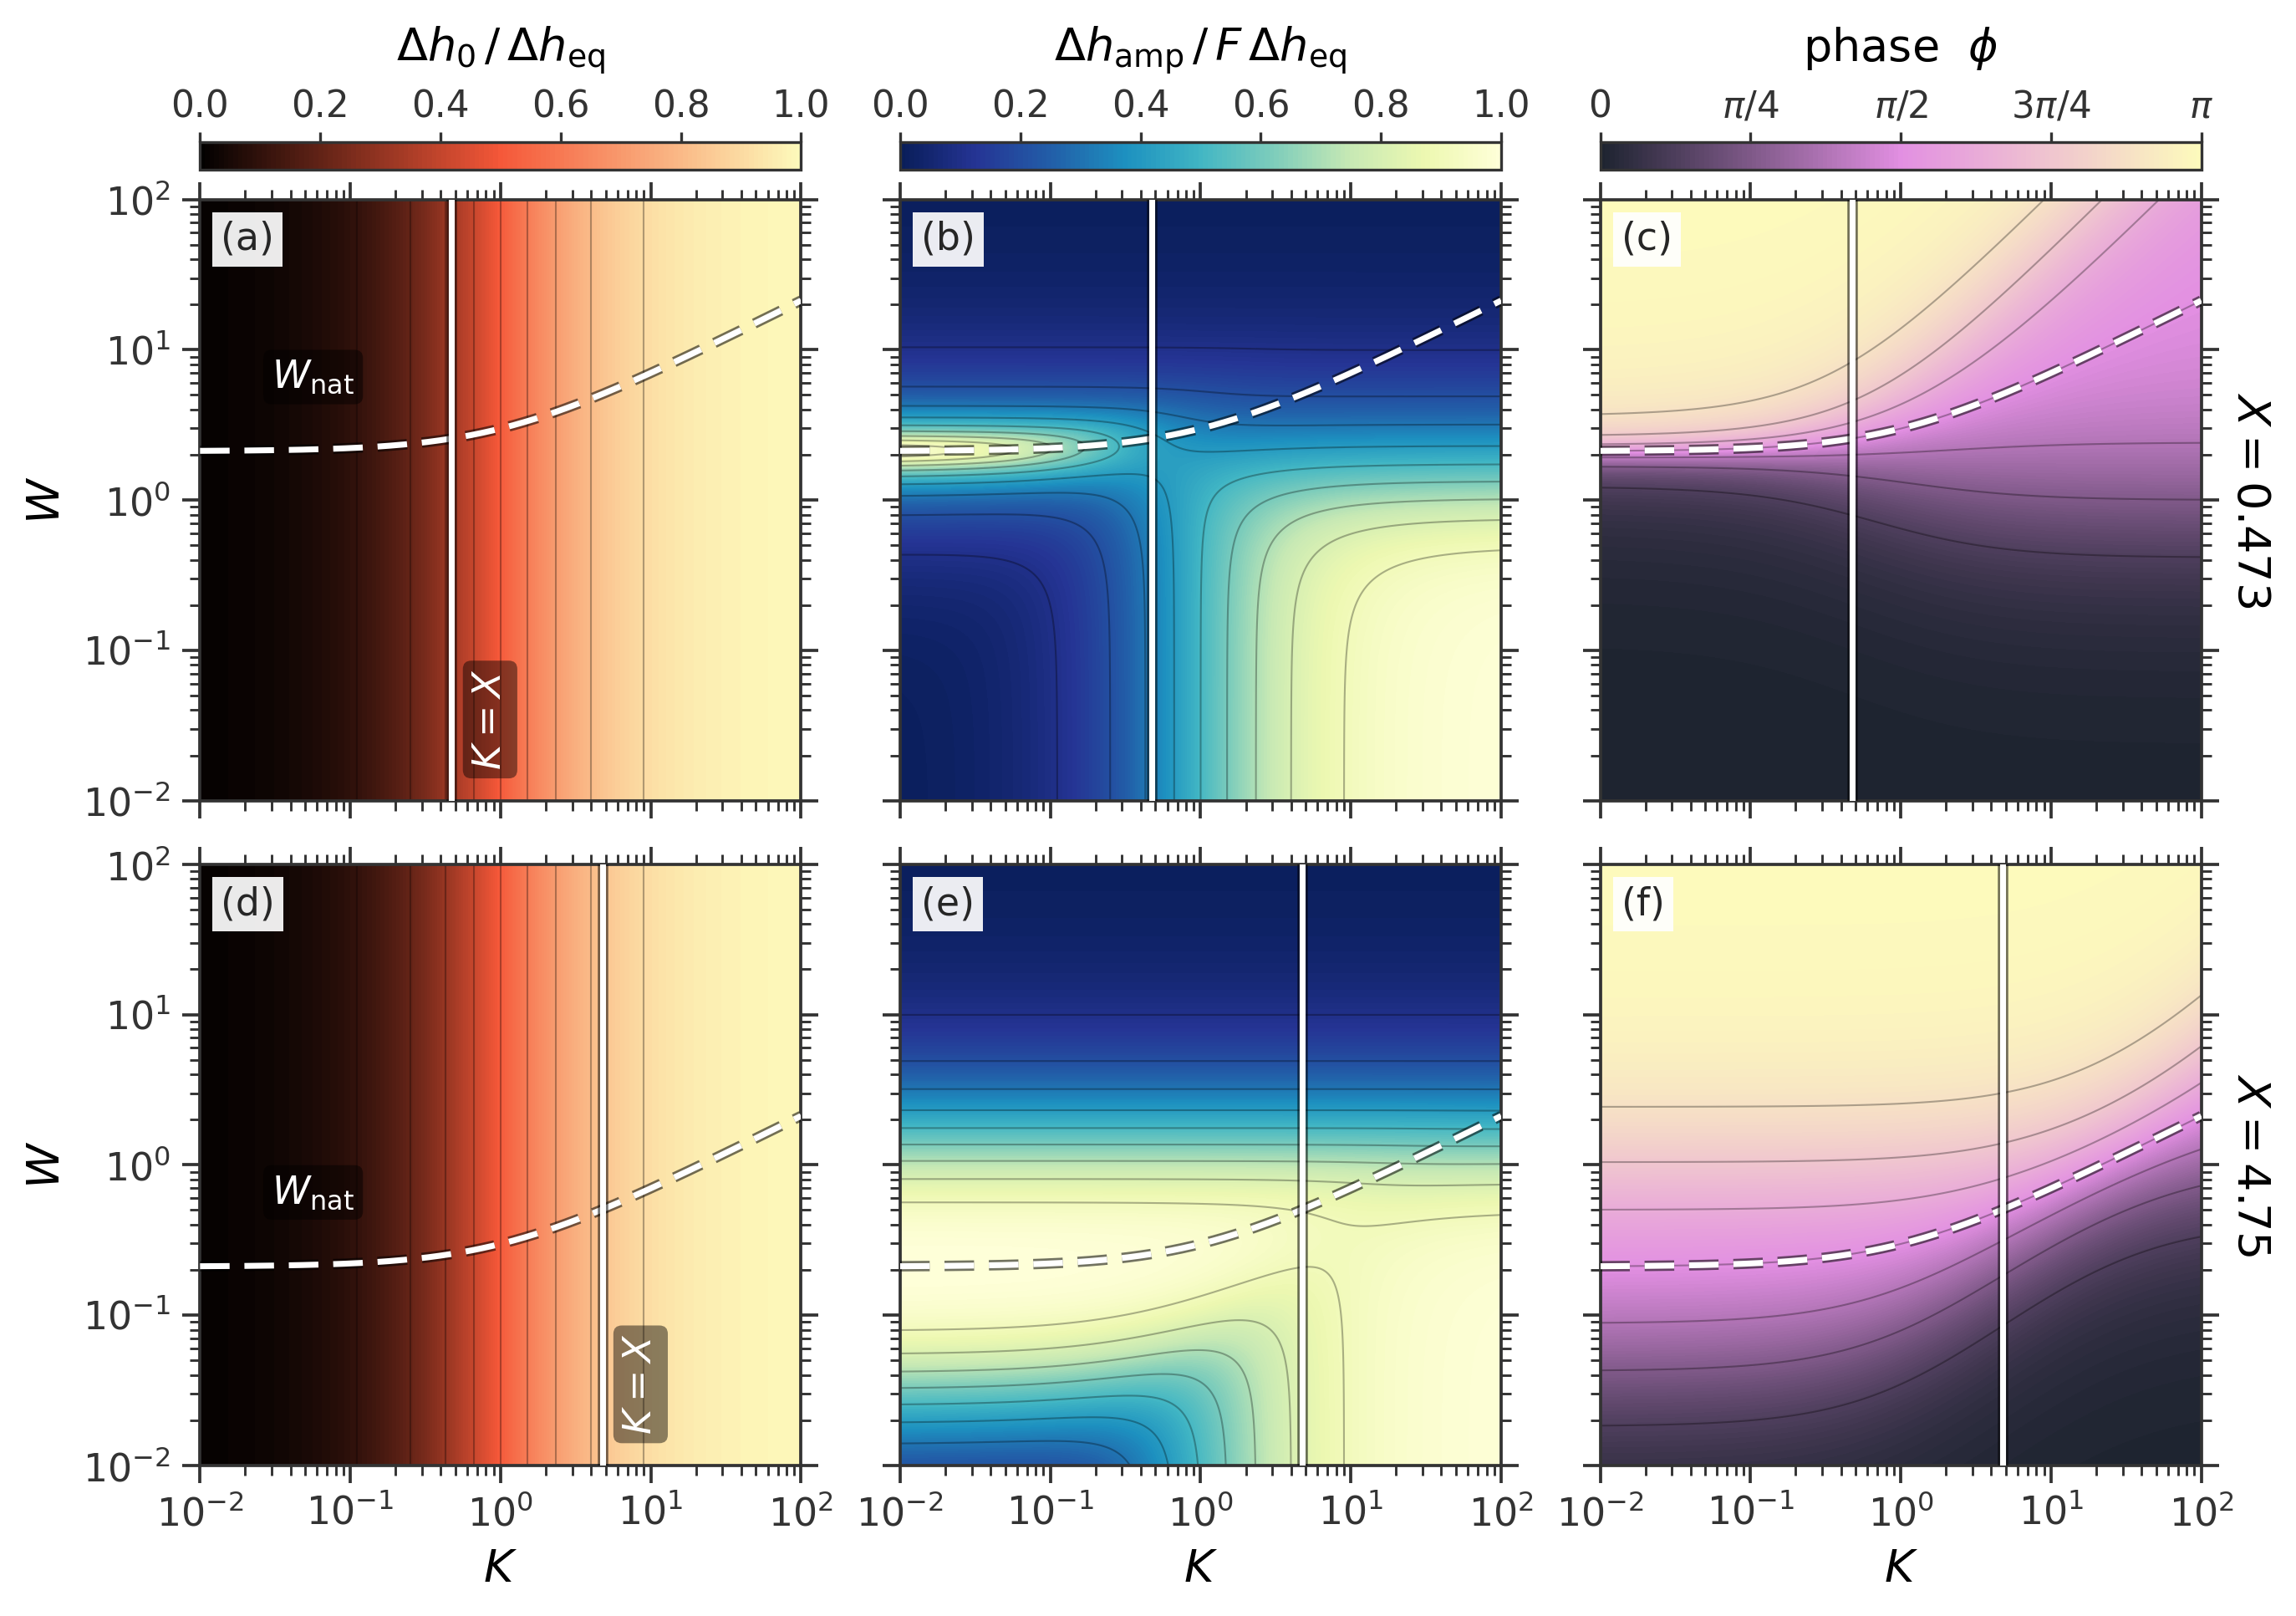
\includegraphics[width=0.85\linewidth]{theory_O2.png}
    \caption{ Response of tidally-locked planets to variable heating, showing forcing normalized time-mean height magnitude ($\Delta h_{\rm o}/\Delta h_{\rm eq}$), its amplitude ($\Delta h_{\rm amp}/ F\Delta h_{\rm o}$), and phase lag of the response using different colorschemes. Results are shown in the $K$--$W$ plane, where $W = \omega \tau_{\rm rad}$, for different values of the third nondimensional parameter $X = \tau_{\rm wave}/\tau_{\rm rad}$. The magnitude response is independent of both $W$ and $X$, and is commensurate with \cite{perez2013atmospheric}. The brown and black dashed lines correspond to natural ($\Omega_{\rm o}$) and resonant ($\Omega_{\rm res}$) frequencies of the system. The solid black line corresponds to the critical damping $K$, to the left of which oscillatory solutions exist, and the system is overdamped to the right. The solid white line ($K = X$) represents separation between the wave dominated inertial regime to the left of it and the drag/rotation dominated regime to the right, where inertia is negligible and the response reduces to a simple relaxation towards the forcing.
}
    \label{fig:foso_theory}
\end{figure*}

We may understand the time-dependent response of the system as follows: gravity-wave adjustment provides the restoring force, while radiative relaxation and drag provide the damping. If the planetary atmosphere is suddenly illuminated with a flash of radiation, the day side would heat up temporarily. This increases the height of the day side which then adjusts itself by propagating throughout as gravity waves, which may interfere with one another sustaining global oscillations only if the effective drag (drag + rotation) is low (large $\tau_{\rm eff}$) and if the heat loss via radiative cooling is relatively slow (large $\tau_{\rm rad}$). The response is the same as the classical spring-mass-dashpot system subject to a delta kick.

In this section, we shall start focussing on systems with \textit{periodically} varying instellation, the central theme of this work --- which resembles a \textit{forced} damped harmonic oscillator. Even though the real nature of variability can be significantly complicated, we start with simpler forms. We assume the forcing to be a simple sine superimposed on a background value and set $f(t) = (1 + F\sin \omega t)$, where $\omega$ is the instellation variation frequency. There is a transient response which we may ignore here  and look at the steady-state response. We obtain solutions of the form
$
   \Delta h(t) = \Delta h_{0} \;+\;  \Delta h_{\mathrm{amp}}\,\cos\bigl(\omega t - \phi\bigr)
    \label{eq:case3_alt_ansatz}
$
to get,
\begin{equation}
    \frac{\Delta h_0}{\Delta h_{\mathrm{eq}}}
    = \left(1 + \dfrac{\tau_{\rm rad} \tau_{\rm eff}}{\tau_{\rm wave}^2}\right)^{-1} = \frac{1}{1+1/K},
    \label{eq:so_mean}
\end{equation}
\begin{align}
   \frac{1}{F} \cdot \frac{\Delta h_{\mathrm{amp}}}{\Delta h_{\mathrm{eq}}}  = \frac{\dfrac{1}{\tau_{\text{rad}}} \sqrt{\dfrac{1}{\tau_{\text{eff}}^2} + \omega^2}}{\sqrt{(\Omega_{\rm o}^2 - \omega^2)^2 + (\gamma \omega)^2}}  \nonumber \\ = \frac{\sqrt{K^2 + W^2 X^4}}{\sqrt{(1 + K - W^2 X^2)^2 + W^2 (X^2 + K)^2}}
   \label{eq:so_amp}
\end{align}
\begin{equation}
    \text{and } \tan \phi = \frac{\gamma \omega}{\Omega_{\rm o}^2 - \omega^2} =  \frac{W(X^2 + K)}{1 + K - W^2 X^2}.
    \label{eq:so_phase}
\end{equation}

Here we have defined two new nondimensional parameters: $W=\omega \tau_{\rm rad}$ is the nondimensional instellation variation frequency and $X=\tau_{\rm wave}/\tau_{\rm rad}$. Thus, the dimensionality of the parameter space is reduced from seven dimensional parameters ($f, g, a, H, \tau_{\rm rad}, \tau_{\rm drag}$, and $\omega$) to just three nondimensional parameters $X, K$ and $W$. The nondimensional natural frequency of the system is $\Omega_{\rm o} \tau_{\rm rad} = \sqrt{(1 + K)/X^2}$. $X=\tau_{\rm wave}/\tau_{\rm rad}$ is the measure of how fast waves cross the planet relative to radiative relaxation. This parameter differentiates various planet types. For example, mildly irradiated Earth-like or other distant planets typically have $X<1$, while strongly irradiated hot Jupiter-like planets have $X>1$, depending on their relative wave speed ($=a/\sqrt{gH}$) which in turn is a function of the size, composition and atmospheric thickness of the planet. For this work we fix the values of $X$ at 0.473 and 4.745 to represent two classes of planets that lie on either size of the $X=1$ boundary; see Table \ref{tab:system_params}.

% The mean part of the planetary contrast \eqref{eq:so_mean} is unaffected by a change in $\omega$ and by $X$. A large value of $K$ corresponds to a planet that is strongly dragged, fast rotating, strongly radiated or any combination of them, all of which helps prevent heat redistribution. On the contrary, a planet with fast wave physics has a low $K$, and has better heat redistribution leading to an erasure of contrasts. The constant part of the contrast normalized by the forcing amplitude is thus seen to increase with $K$ peaking at 1. The amplitude of variation in planetary temperature behaves in a similar manner, except it is also affected by the frequency of instellation variation. When $W$ or $\omega$ is large, the instellation fluctuates fast and the planet does not get enough time to adjust to the radiation leading to a muted amplitude irrespective of the value of $K$, while low $W$ allows the system to respond appropriately, leading to higher amplitudes.

\subsection{Inertial and damped responses}\label{sec:in_dam_resp}

At this point, it is useful to determine one last scale: the characteristic timescale on which the height field itself evolves. Comparing the scales of the unsteady ($\partial h'/\partial t$) and the height advection (mass flux, $H\nabla\cdot\mathbf{u}'$) terms in equation \eqref{eq:lin_cont} gives the following timescale for the flow in general,
\begin{equation}
    \frac{\Delta h}{\tau_{\rm o}} \sim \frac{HU}{a} \implies \tau_{\rm o} \sim \tau_{\rm adv} \cdot \frac{\Delta h}{H} = \frac{\tau_{\rm wave}^2}{\tau_{\rm eff}} \label{eq:scale_time}
\end{equation}
where $\tau_{\rm adv} = a/U$ is the advection timescale, or the timescale over which winds traverse across the planet. The unsteady term ($\partial \mathbf{u}'/\partial t$) in the momentum equation \eqref{eq:lin_mom_unsteady} is significant whenever its scale is much greater than that of the effective drag term, $U/\tau_{\rm o} \gg U/\tau_{\rm eff}$, or $\tau_{\rm o} \ll \tau_{\rm eff}$. Substituting the timescale $\tau_{\rm o}$ from equation \eqref{eq:scale_time}, this condition becomes
\begin{equation}
    \tau_{\rm wave} \ll \tau_{\rm eff},
    \label{eq:wavelleff}
\end{equation}
which is the same condition as inequality \eqref{eq:condt_inertial}. This is expected because the unsteady and advective terms are components of the material derivative and hence have the same scaling. When the condition in \eqref{eq:wavelleff} is satisfied, rotation and drag are weak and cannot damp gravity wave perturbations from reverberating across the planet, and the height field simply relaxes towards the forcing giving rise to linearized inertial physics. When waves dominate new behavior emerges through constructive or destructive interference leading to resonances, as we shall see further. 

Figure \ref{fig:foso_theory} shows the time-mean height magnitude, its amplitude, and phase of planetary response for the two different values of $X$ mentioned above and will be compared with simulations in the upcoming section. So far as the constant part of the solution, equation \eqref{eq:so_mean}, is concerned, it is exactly what has been derived from scaling laws in Section \ref{sec:steady_scaling} in equation \eqref{eq:scale3}, which is expected in the absence of variable irradiation. The dynamical response comes from the time varying effect. The first thing to note is the region in $K-W$ space where the inertial physics dominates. This is demarcated by the solid white line $K=X$, which is equivalent to the condition in equation \eqref{eq:wavelleff} in dimensionless form. To the left of the white line, $K < X$ or $\tau_{\rm wave} < \tau_{\rm eff}$, i.e.\ gravity waves traverse the planet before they are damped. This supports a wave-driven resonance. Conversely, for $K > X$ (right of the white line) the wave timescale is too large and the drag too strong. The white line thus separates a wave-active inertial regime from a drag-dominated regime in which the restoring force is ineffective and the planet merely relaxes towards the instantaneous forcing. Outside of the inertial regime, the unsteady momentum term can be ignored, establishing a balance between pressure gradient and the effective drag. This reduces the system further to first order, where it merely represents a periodically forced and linearly damped system that does not exhibit any resonance phenomena. Since this happens to the right of the $K=X$ line, the first order theory will be valid for the entire $K-W$ parameter space when $X \to 0$, pulling the white line all the way to the left. Now, equations \eqref{eq:so_amp} and \eqref{eq:so_phase} reduce to $\left[(1+1/K)^2 + W^2\right]^{-1/2}$, and $\tan\phi = W/(1+1/K)$, which is the response of a system with no restoring force at all.

% This line closely follows the black solid line that separates regions having oscillatory versus overdamped solutions.

The second thing to note is that the inertial regime ($K << X$) features a local maxima in frequency space corresponding to the resonance. In this regime when $K$ tends to 0, we find the dimensionless natural frequency $W_{\rm o}$ to be equal to $1/X$. Coming to dimensional quantities, this condition holds precisely when the instellation variation time matches the wave timescale of the planet. Thus, when the system is purely inertial, the natural frequency of the system is the wave frequency. This can also be concluded from equation \eqref{eq:nat_freq_damp} when $\tau_{\rm eff}, \tau_{\rm rad} \to 0$. The correspondence can be seen at low values of $K$ for respective $X$, where the white dashed lines representing natural frequency asymptotes to become parallel to the x-axis close to $W=1/0.0473\sim2$, and $1/4.75\sim0.2$ for the two values of $X$, respectively. Finally, the phase lag of the system can take up values larger than $\pi/2$ as the theoretical limit reaches $\pi$ symbolizing a complete out-of-phase response. Note that this phase is not the hotspot offset from the substellar point but the time difference between the peak of instellation and planetary maxima. {\color{red} However, as we shall see later in simulations with appended discussion in \S \ref{sec:role_of_nonlinearities}, the phase lag never goes beyond $\pi/2$ due to the presence of nonlinearities in the system.}

{\color{teal} Note on the form of forcing? The forcing term is of the form $\Delta h_{\rm eq}[\dot{f}/\tau_{\rm rad} + f/(\tau_{\rm rad}\tau_{\rm eff})]$ rather than simply $\Delta h_{\rm eq} f/\tau_{\rm rad}$. This is because retaining the unsteady term in the momentum equation introduces an additional time derivative of the forcing function $f(t)$ in the governing equation. The system therefore responds both to the instellation and to its rate of change, and it is the $\dot{f}$ contribution that produces the $W^2X^4$ term in the numerator of \eqref{eq:so_amp}.}

Thus, the response of tidally locked planets to time-variable irradiation is that of a damped harmonic oscillator, in which gravity-wave adjustment provides the restoring force while radiative relaxation and drag provide the damping. Whether the oscillator rings or is overdamped is set by $K$ relative to $X$, and the resonance that follows is the central prediction of the theory. In the next section we test the efficacy of our theory through simulations and also investigate the role of nonlinearities and how the system behaviour departs from the linearized theory presented above.

\subsection{Assumptions and limitations of the analytical framework}\label{sec:assu_lim}

\begin{figure}
    \centering
    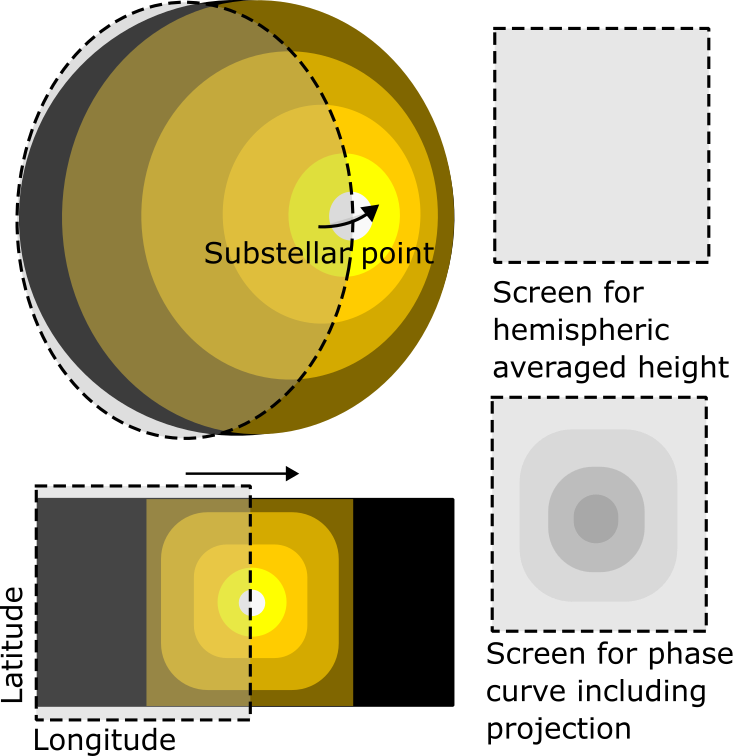
\includegraphics[width=0.9\linewidth]{schem_hemi.png}
    \caption{Typical equilibrium temperature distribution of a tidally-locked planet in two different representations, spherical and rectangular, showing the substellar point at the centre of the day side, and hemispheric screens for calculating the hemispheric averaged height and phase curves. The rectangular representation also shows the latitude, longitude and the night side. The arrows show the direction in which the screen moves to calculate the respective quantities. The screen for hemispheric averaged height is plain, while the second includes a projection to account for ray tracing effects needed for phase curve predictions.}
    \label{fig:schem_hemi}
\end{figure}

The analytical results rest on several simplifying assumptions. Firstly, the effective drag approximation combines the Coriolis term and Rayleigh drag into a scalar $\tau_{\rm eff}^{-1} = f\sin\phi_0 + \tau_{\rm drag}^{-1}$ adequately estimates global heat redistribution \citep{perez2013atmospheric}, but discards the directional information needed to predict the eastward vs.\ westward direction of hotspot oscillations. The simulations retain the full Coriolis term and reproduce this transition. Second, we assume a cosine ansatz for the trial solution $h'(x,t)=\Delta h(t)\cos(kx)$ that is symmetric about the substellar point implying purely substellar to antistellar point flow, so the theory does not predict any spatial hotspot displacement. The actual offset arises from the 2D Matsuno-Gill response \citep{HammondPierrehumbert2018,pierrehumbert2019atmospheric}, which is not included in this 1D framework. Third, we retain only the gravest wave mode $k=1/a$ spanning the entire planet. At fast rotation, the Rossby deformation radius $L_d = c/\sqrt{f} \ll a$ and higher harmonics become energetically important, causing the theory to overestimate the planetary response (see simulation results later). Fourth, the meridional gradients are simplified by assuming periodic boundary conditions along longitudes, reducing the problem to a 1D zonal diffusion equation. This equatorial-strip approximation breaks down at fast rotation where off-equatorial Rossby wave structure becomes significant. Finally, the linearized theory neglects the term $\mathbf{R}$ (equation~\ref{eq:SW_mom}) which is responsible for equatorial superrotation \citep{ShowmanPolvani2011}, is omitted from linear calculations. The theory therefore cannot predict the equatorial jet, but the large-scale pressure-drag balance remains a reasonable approximation even in its presence.

Despite these limitations, the large-scale thermodynamic response — including the day--night contrast, oscillation amplitude, and phase lag — is well captured by the theory, as confirmed by the simulations in the following section.

\section{Numerical simulations}
\label{sec:simulations}

Now we turn to full computational solutions to our shallow water equations without applying the simplifying assumptions in the previous section. These hydrodynamical simulations help us identify the limits of our theory for the time-dependent planetary response to periodically varying irradiation and by their inherent 2-dimensionality also capture global flow patterns and their variability which cannot be studied using the reduced theory above.

\subsection{Framework}

Equations (\ref{eq:SW_mom}) and (\ref{eq:SW_mass}) are solved numerically using Dedalus3 \citep{burns2020dedalus}, a flexible pseudo-spectral code for symbolic equation entry. We discretize the 2-D domain on a sphere basis and evolve the system using an SBDF2 timestepper. The simulation resolution is $32 \times 16$ (longitude $\times$ latitude), which, while low, sufficiently captures the core physical phenomena. This resolution corresponds to a minimum resolvable horizontal scale of $\sim$1000\,km for an Earth-like planet — adequate for the dominant wavenumber-1 day--night response but insufficient to resolve structures smaller than the equatorial Rossby deformation radius at the fastest rotation rates explored. We admit that increasing the resolution would improve the accuracy of the simulations, but avoided doing so in the interest of exploring a larger parameter space. Our code was verified by reproducing results from existing literature \citep{perez2013atmospheric, penn2017thermal, ohno2019atmospheres} and is structurally the same as in \cite{Banik2025}.

The tidally locked height field is relaxed towards an equilibrium profile $h_{\text{eq}}$ as shown in Figure~\ref{fig:schem_hemi}, the intensity of which is periodically varied. The form of the equilibrium height field is given by

\begin{align}
    h_{\rm{eq}}(\lambda,\phi,t) = H + \Delta h_{\rm eq}\cdot\frac{\mathcal{R} + |\mathcal{R}|}{2} \left(1 + F \cos \omega t \right) \nonumber
    \\
    \text{where} \hspace{2mm} \mathcal{R} = \cos \lambda \cos\phi.
\end{align}

Here, $\rm{H}$ is the nightside thickness, $\Delta \rm{h_{eq}}$ is the forcing day-night contrast, and $F$ and $\omega$ are the instellation fluctuation amplitude and frequency. The factor $(\mathcal{R} + |\mathcal{R}|)/2$ isolates hemispheric irradiation \citep{dobrovolskis2009insolation}.

\begin{figure}
    \centering
    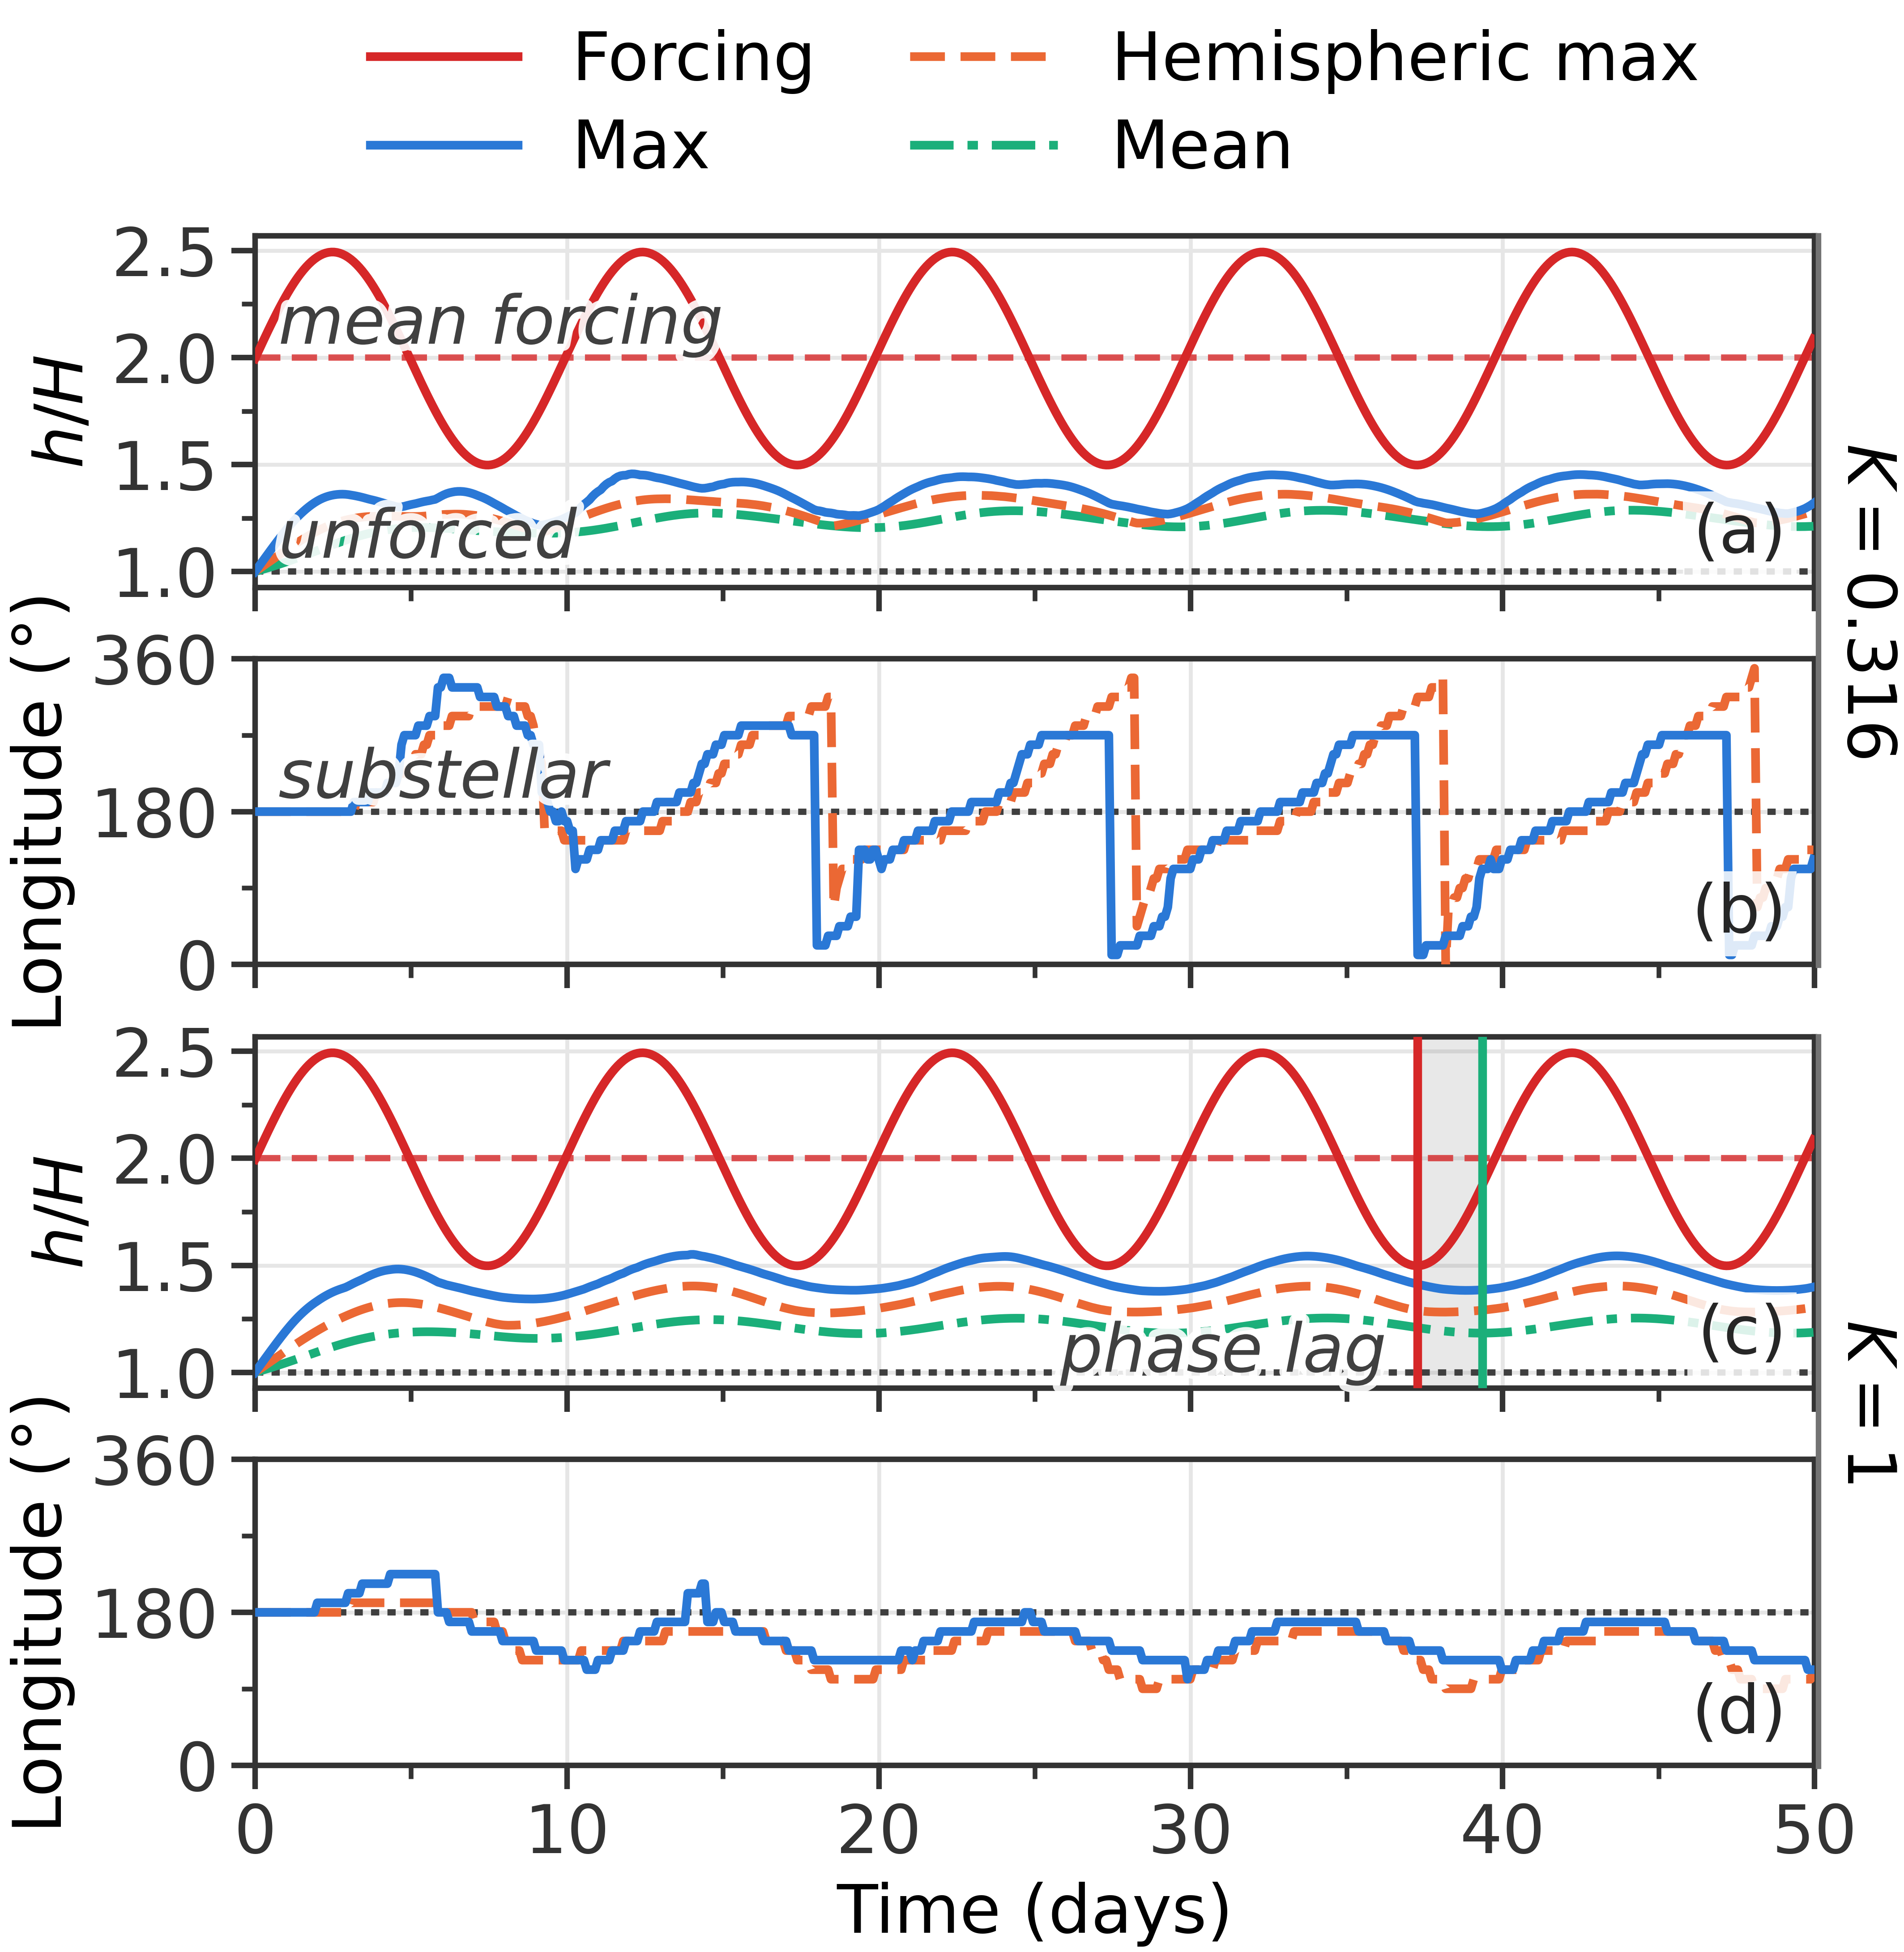
\includegraphics[width=\linewidth]{response_single_column.png}
    \caption{Nonlinear shallow-water response to time-varying instellation for two
rotation rates of Earth-like planets; see Table \ref{tab:system_params}. Panels (a) and (c) show the height field as $h/H$ --- the
forcing maximum, the global maximum, the hemispheric (observer-weighted)
maximum and the global mean; the dotted line is the unforced state $h/H = 1$
and the dashed red line the mean forcing $(H+\Delta h_{\rm eq})/H$. Panels (b)
and (d) give the longitude of the global and hemispheric maxima, with the
substellar point dotted. The top pair is $K = 0.316$ (rotation period
$26.4$~d), the bottom pair $K = 1$ ($7.40$~d); both share $W = 3.16$ and a
forcing amplitude $\Delta h_{\rm eq}/H = 1$ modulated at the instellation
period $P_{\rm inst} = 9.93$~d. Only the first 50~d ($\sim$5 cycles) of the 99.35~d run are
shown.}
    \label{fig:run_diag}
\end{figure}

\begin{figure*}
    \centering
    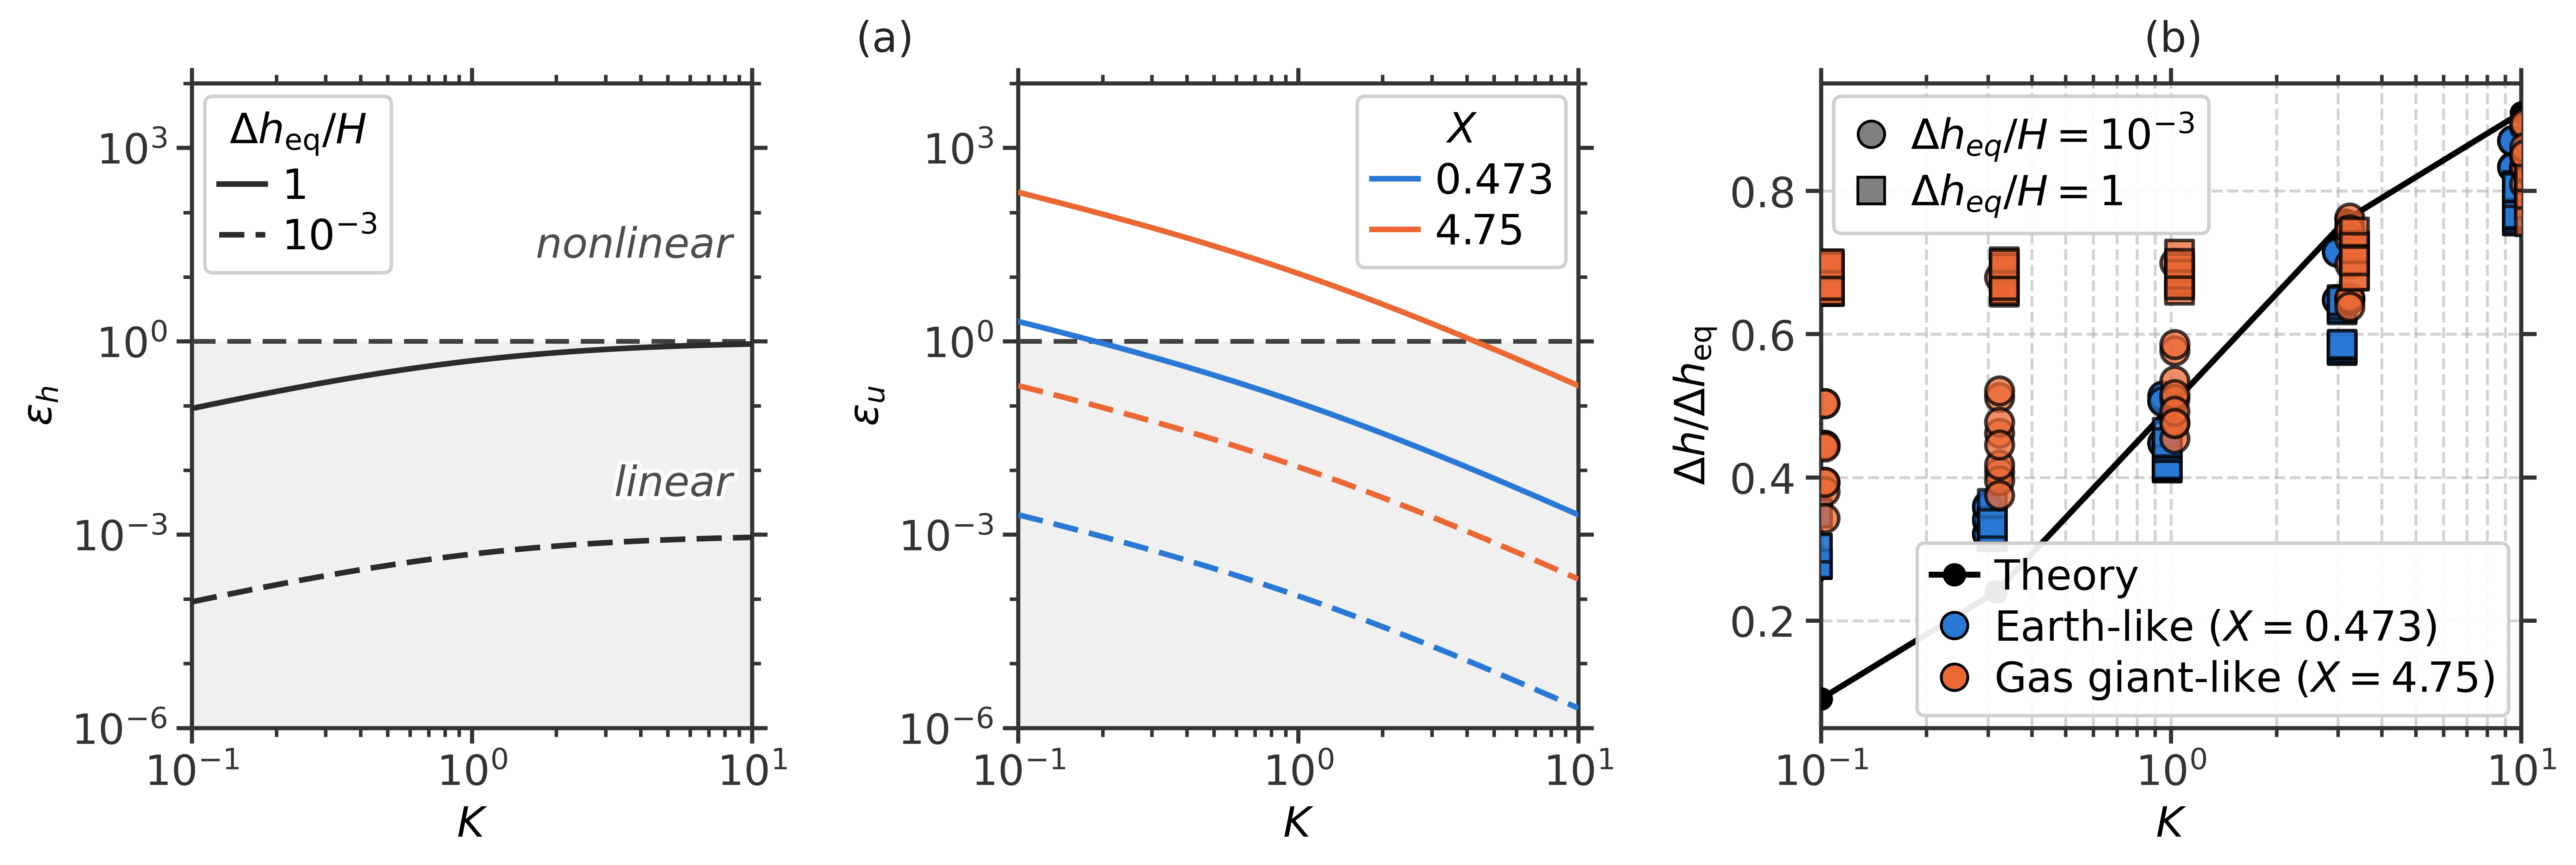
\includegraphics[width=\linewidth]{regime_and_contrast.png}
    \caption{(a) Magnitude of linearity constants in inequalities \eqref{eq:lin_condt1} and, \eqref{eq:lin_condt2} with $K$ for different system parameters assumed in this work. Note that $X=\tau_{\rm wave}/\tau_{\rm rad}$. (b) Variation of $\Delta h/\Delta h_{\rm eq}$ with $K$ for different Earth-like and gas giant planetary system parameters from all simulations performed in the following section compared with theoretical predictions. The linear (circles) and nonlinear (squares) regime simulations are horizontally offset by small quantity for the ease of visualization. Linear regime simulations match the theory very well, while the nonlinear regime simulations show quantitative differences, as expected.}
    \label{fig:regime_constrast}
\end{figure*}


\subsection{Diagnostics}
Each run produces timeseries of global height and velocity fields. These are post processed to obtain the quantities that can be compared with the theory above. From the global height field we obtain the timeseries of the \textit{maximum} height, the global \textit{mean} height and, the \textit{hemispheric averaged} height as can be see in Figure \ref{fig:run_diag}. The time-mean magnitude of planetary response is calculated by taking the average of the peak and trough of the \textit{maximum} height timeseries after the simulation is out of it's transient evolution phase and relaxed to a oscillating steady state, typically over the last three oscillation cycles of every simulation. The \textit{amplitude} is modulus half the difference between the peak and trough of the same. The statistical steady state is identified by tracking the time-averaged kinetic energy of the flow to have reached a constant value. Finally, the \textit{phase} is obtained by calculating the temporal offset between the troughs in instellation and \textit{mean} height and converting it to radians; see third panel in Figure \ref{fig:run_diag}. The reason for choosing the mean height here is that it has a smoother sinusoidal structure than maximum height, especially for inertia dominated cases where interacting waves interfere to create complicated responses. 

We also obtain another estimate of the global height field, the \textit{hemispheric averaged} height. It is calculated as an average of the height field over a longitudinal extent of $\pi$ radians, the face of the planet centered at each individual longitude, and is a more accurate metric when comparing with observations that average the light coming from the exposed planetary hemisphere. See the projection used for this calculation in Figure \ref{fig:schem_hemi}. We also obtain the longitudinal location of maximum height and the maximum hemispheric averaged height to track the motion of the real and observationally apparent hotspots. 

\subsection{Exploration parameters}
\label{sec:exploration}

\begin{table*}[ht]
\centering
\caption{Physical parameters and timescales corresponding to the simulations presented. The table shows a total of 100 simulations, each of which are conducted at two different values of $\Delta h_{\rm eq} = 10^{-3} H$ and $H$, representing the linear and nonlinear regimes described above, resulting in a total of 200 simulations.}
\begin{tabular*}{\textwidth}{@{\extracolsep{\fill}}llll}
\toprule
\textbf{Parameter} & \textbf{Symbol} & \textbf{Earth-like} & \textbf{Gas giant-like} \\ 
\midrule
Surface gravity & $g$ & $9.81\,\text{m}\cdot\text{s}^{-2}$ & $10\,\text{m}\cdot\text{s}^{-2}$ \\
Scale height & $H$ & $100\,\text{m}$ & $4 \times 10^{5}\,\text{m}$ \\
Radiative timescale & $\tau_{\text{rad}}$ & $5\,\text{days}$ & $0.1\,\text{days}$ \\
Instellation variation & $\tau_{\text{instel}}$ & $3.14 - 314\,\text{days } (\times 5)$ & $0.06 - 6.28\,\text{days }  (\times 5)$ \\
Wave timescale (derived) & $\tau_{\text{wave}}$ & $2.365\,\text{days}$ & $0.4745\,\text{days}$ \\
Wave-to-radiative timescale ratio (derived) & $X$ & $0.473$ & $4.745$ \\
\addlinespace
\midrule
\textbf{Scenario} & \textbf{Rotation Period ($P_{\text{rot}}$)} & \textbf{Drag Timescale ($\tau_{\text{drag}}$)} & \textbf{No. of sims} \\ 
\midrule
\textbf{A: Earth-like} & & & \\
- Batch 1 & $140\,\text{days}$ & $0.11 - 22.373\,\text{days } (\times 5) $ & 25 \\
- Batch 2 & $0.7 - 140\,\text{days}$ & $22.373\,\text{days } (\times 5)$ & 25 \\
\addlinespace
\textbf{B: Gas giant} & & & \\
- Batch 3 & $282\,\text{days}$ & $0.22 - 45\,\text{days } (\times 5)$ & 25 \\
- Batch 4 & $1.42 - 282\,\text{days}$ & $45\,\text{days } (\times 5)$ & 25 \\
\bottomrule
\label{tab:system_params}
\end{tabular*}
\end{table*}

% \begin{table*}[ht]
% \centering
% \caption{Derived Scenarios (Grid Resolution: $5 \times 5$)}
% \begin{tabularx}{\textwidth}{lXXX}
% \toprule
% \textbf{Scenario} & \textbf{Rotation Period ($P_{\text{rot}}$)} & \textbf{Drag Timescale ($\tau_{\text{drag}}$)} & \textbf{Key Ratio} \\ 
% \midrule
% \textbf{A: Earth-like} & & & \\
% - Case 1 (Fast Rot.) & $140\,\text{days}$ & $22.373\,\text{days}$ & $\tau_{\text{drag}}/P_{\text{rot}} \approx 0.16$ \\
% - Case 2 (Slow Rot.) & $140\,\text{days}$ & $22.373\,\text{days}$ & $P_{\text{rot}}/\tau_{\text{drag}} \approx 6.26$ \\
% \addlinespace
% \textbf{B: Gas giant} & & & \\
% - Case 3 (Fast Rot.) & $282\,\text{days}$ & $45\,\text{days}$ & $\tau_{\text{drag}}/P_{\text{rot}} \approx 0.16$ \\
% - Case 4 (Slow Rot.) & $282\,\text{days}$ & $45\,\text{days}$ & $P_{\text{rot}}/\tau_{\text{drag}} \approx 6.27$ \\
% \bottomrule
% \end{tabular*}
% \end{table*}


We simulate 25 planets that span the entire nondimensional $K-W$ parameter space sampling 5 equally log-spaced values each between $10^{-1}$ and $10^1$;  see individual panels in Figure \ref{fig:earth_analog}. We use two different magnitudes for the base relative forcing $\Delta h_{\rm eq}/H = 10^{-3}$ and $1$, respectively to span linear and nonlinear behavior. Figure \ref{fig:regime_constrast}(a) plots the linearity constants $\varepsilon_h$ and $\varepsilon_u$ as a function of $K$ for two different forcing magnitude $\Delta h_{\rm eq}/H$, and two different classes of planetary parameters, the first corresponding to Earth-like planets for which $X=0.473$ \citep{penn2017thermal,ohno2019atmospheres,Banik2025}, and the other corresponding to typical close-in gas giants for which $X=4.75$ \citep{perez2013atmospheric}. We see that the momentum condition is decisively nonlinear for the latter group at strong forcing for most values of $K$ (orange solid line), while the other cases are relatively linear. The differences in their response to variable irradiation shows up distinctly when hotspot locations are analyzed later in the paper.

The fractional amplitude $F$, is kept at 0.5 to elicit significant response as it scales linearly with $F$. We run these in two batches with $X=0.473$ and 4.75, defining different ratios of radiative and wave adjustment strengths. The first corresponds to smaller Earth-like planets, while the later uses the parameter set in \cite{perez2013atmospheric} applicable to gas giants; see Table \ref{tab:system_params}. 

Here, we recall that in the linearized theory we have assumed the Coriolis and drag terms to be combined into the effective drag term for simplification. However, their effects on the global flow patterns are distinct due to the nature of the individual terms --- the Coriolis term leads to latitudinal variations being stronger closer to the poles and weaker at the equator, while the drag depends only on the velocity and the constant $\tau_{\rm drag}$. For this reason, we vary $K$ by varying both rotation and drag individually, to study if contrast properties are actually significantly affected by them. Finally, we vary $W$ by changing the instellation variation frequency. All permutations included, we have a suite of 200 simulations ($25 \times 2 \times 2 \times 2$), the results of which are presented below. The details of the planetary parameters and total number of runs are given in Table \ref{tab:system_params}.

\subsection{Results and discussion}

% \begin{figure}
%     \centering
%     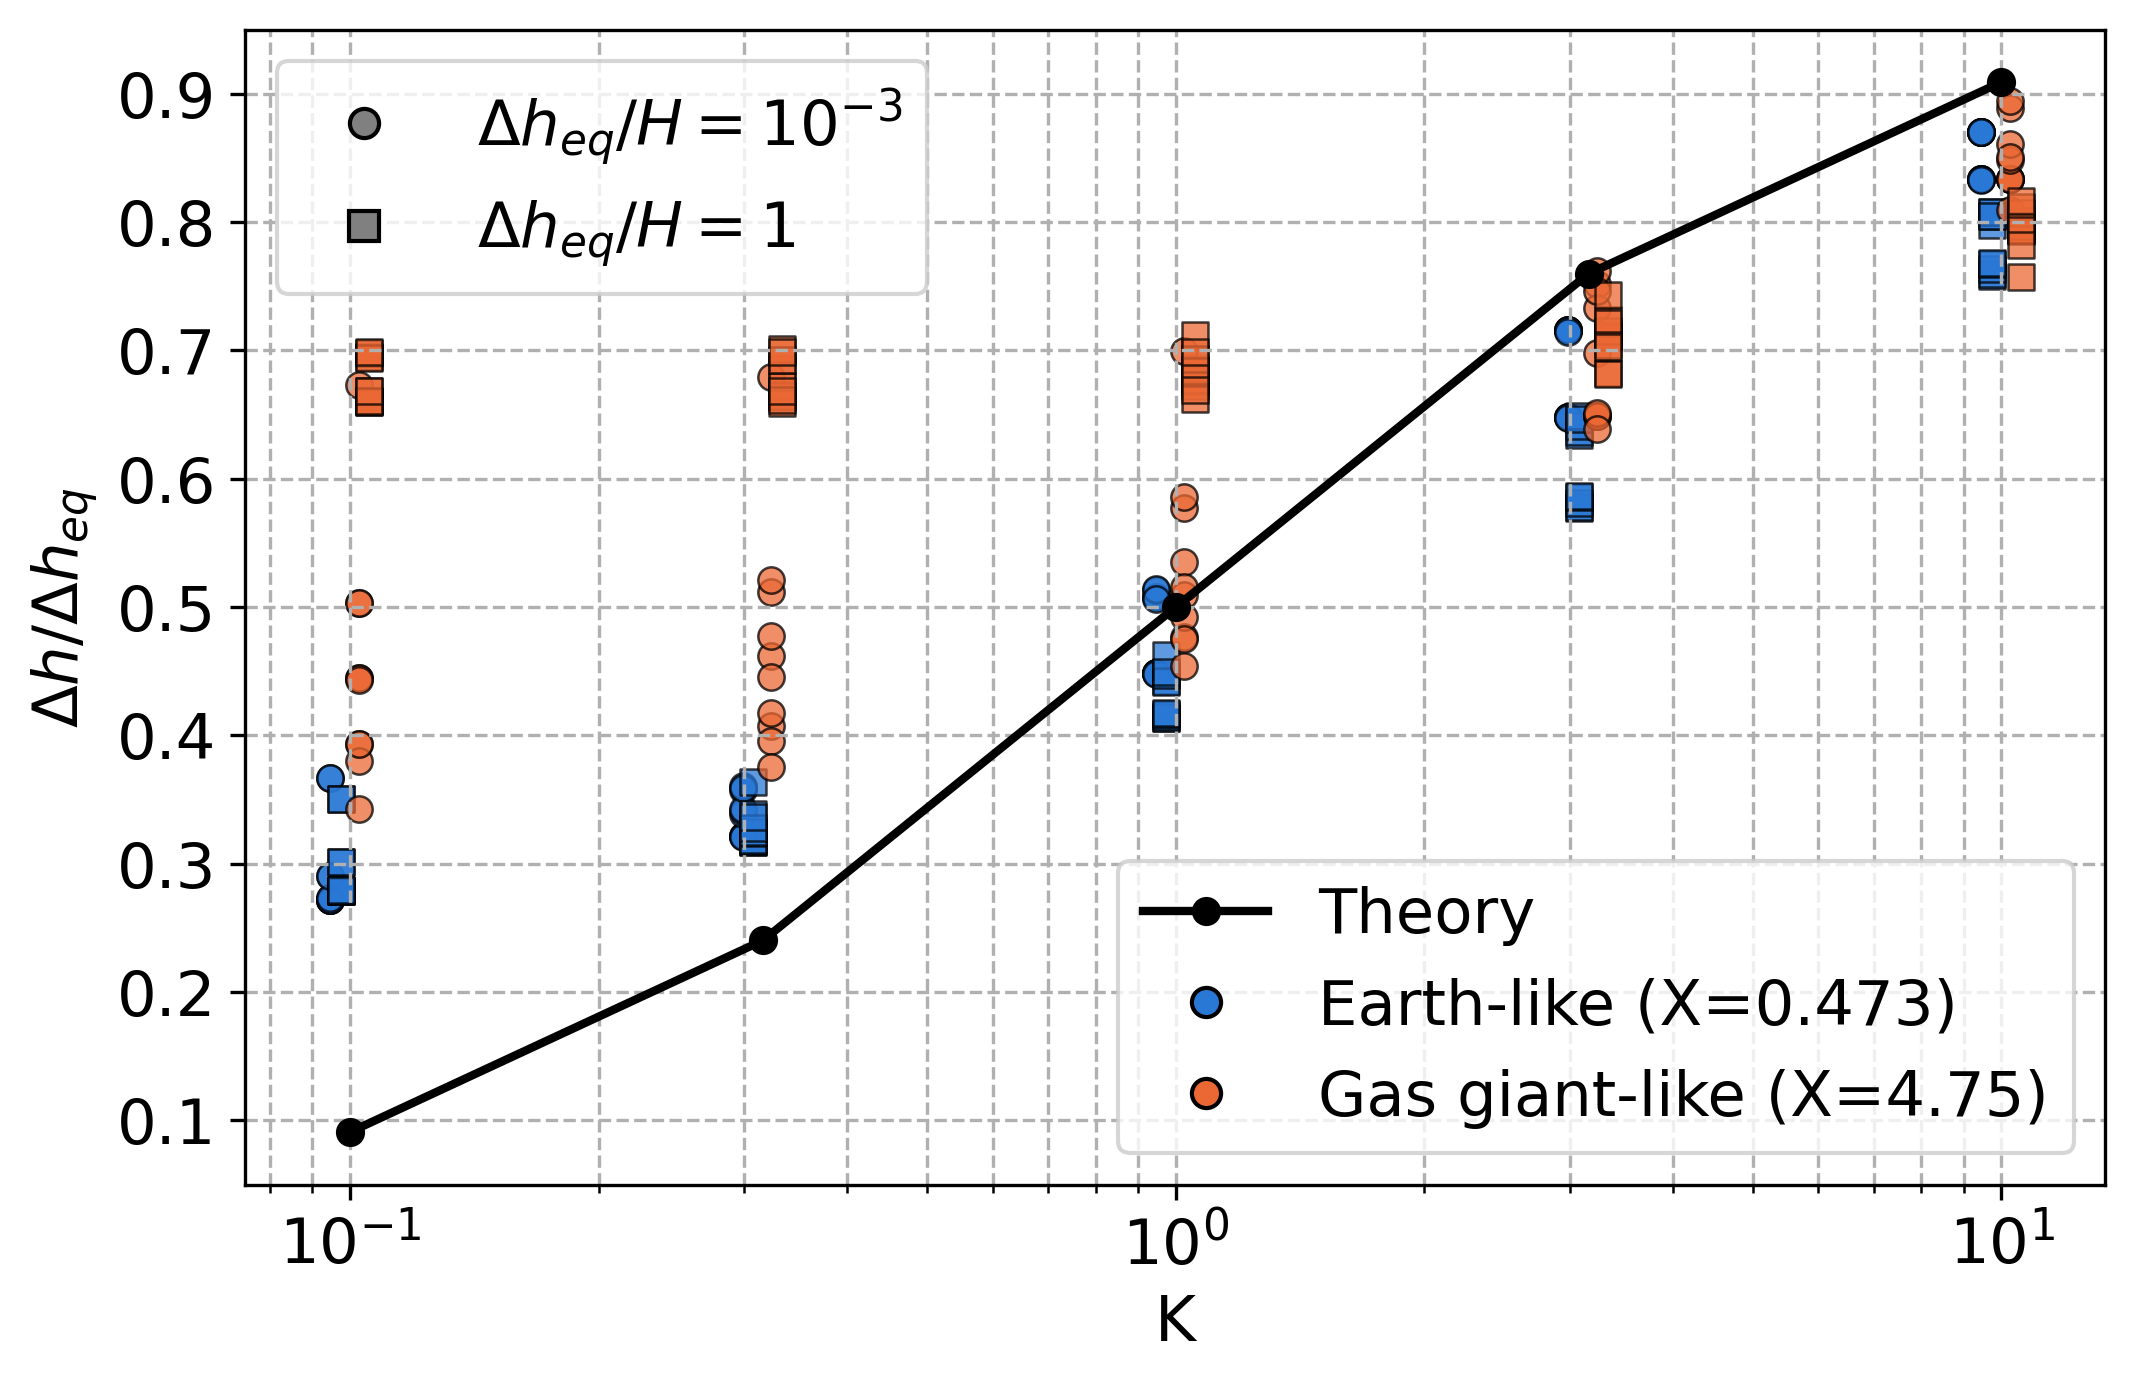
\includegraphics[width=\linewidth]{delta_h_vs_K.png}
%     \caption{Variation of $\Delta h/\Delta h_{\rm eq}$ with $K$ for different Earth-like and gas giant planetary system parameters from all simulations performed in the following section compared with theoretical predictions. The linear (circles) and nonlinear (squares) regime simulations are horizontally offset by small quantity for the ease of visualization. Linear regime simulations match the theory very well, while the nonlinear regime simulations show quantitative differences, as expected.}
%     \label{fig:delta_h_vs_K}
% \end{figure}

In this section we present the results from our numerical simulations and discuss the implications of the same for our theory. Figure \ref{fig:regime_constrast}(b) compares the theoretical contrast magnitude nondimensionalized by the forcing $\Delta h_{\rm eq}/H$ with results from the suite of numerical experiments spanning Earth-like and gas giant-like parameter choices. Data points correspond to simulation results (circles for the linear regime, squares for nonlinear runs) while the solid line shows the theoretical prediction from the linearized shallow-water theory. The theory underpredicts contrasts for lower values of $K$ or in the inertial regime and overpredicts the same in the opposite limit. However, the increasing trend of contrast with $K$ is consistent and demonstrates good agreement between theory and simulations. The linear regime Earth-like cases show a better match, while systematic departures are observed in the nonlinear cases especially at low $K$, highlighting the possible role of nonlinear processes in enhancing the height contrast. {\color{red} (What does PBS13 other literature say?)}

\subsubsection{Typical Earth-like planets}
\label{sec:earth_like}

\begin{figure*}
    \centering
    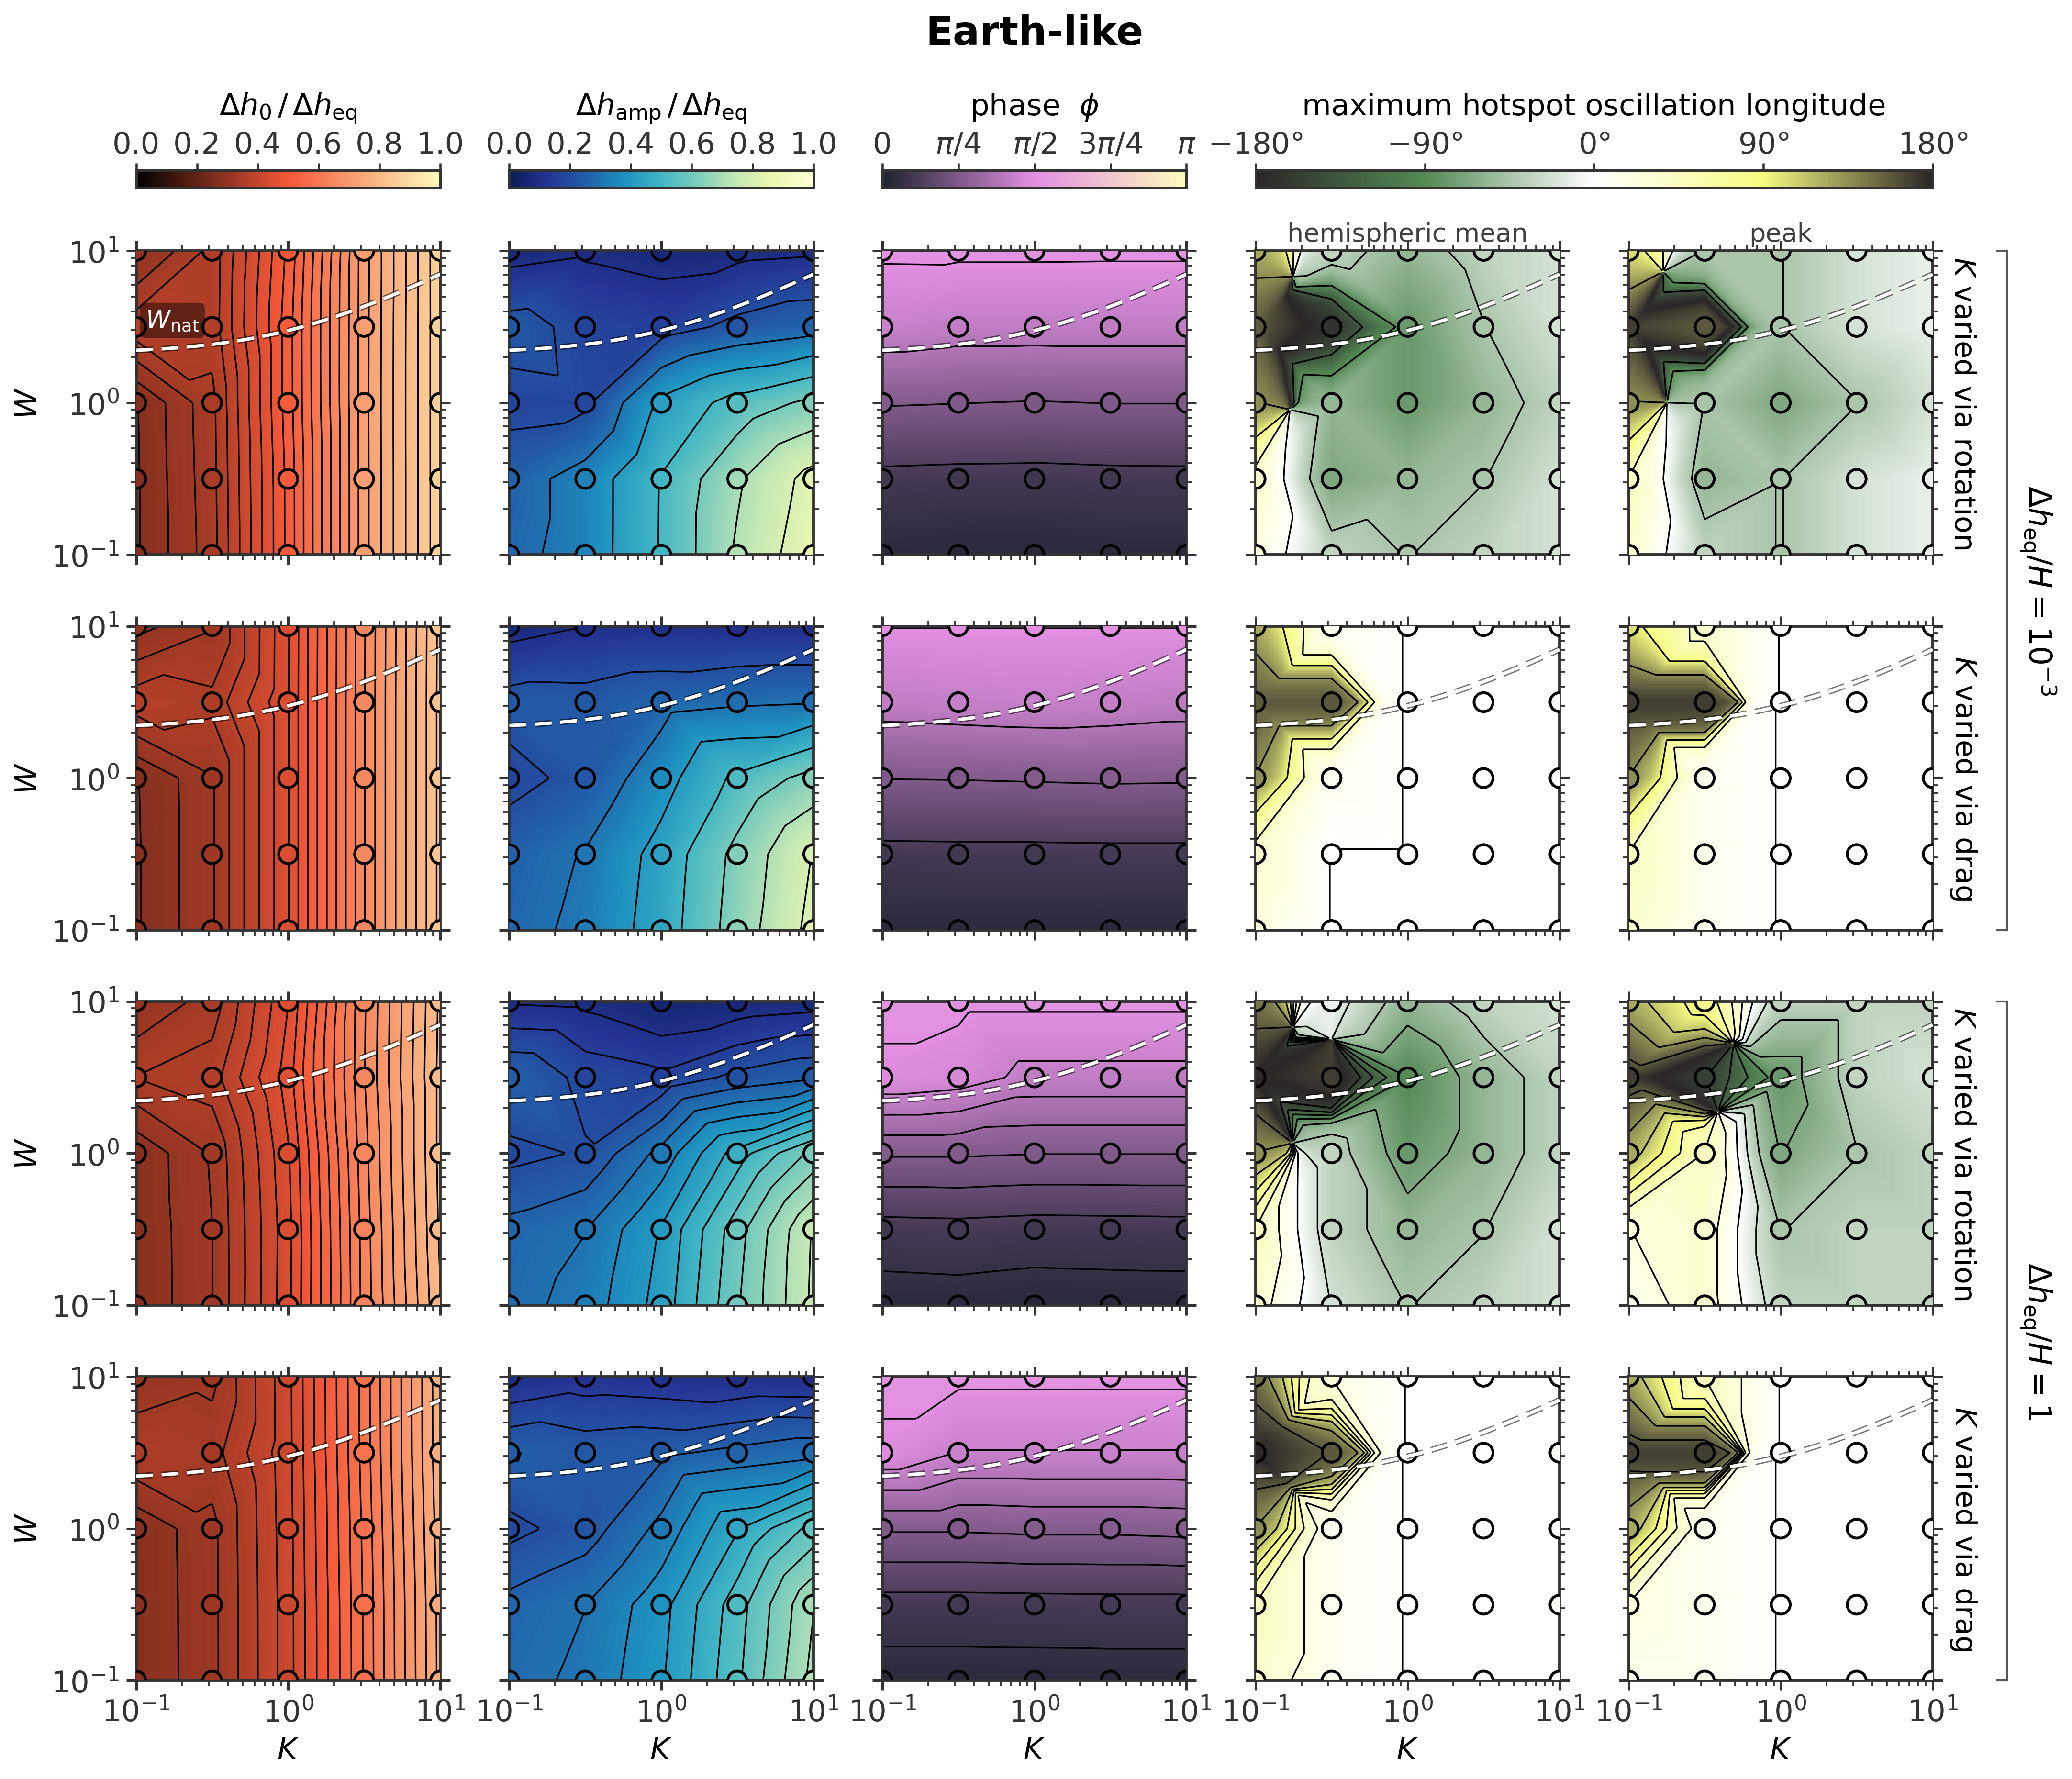
\includegraphics[width=\linewidth]{fig4_sim_earthlike.png}
    \caption{Suite of simulation results for an tidally-locked Earth-analog planet, showing the time-mean height magnitude, its amplitude, phase  and maximum oscillating hotspot shift from the substellar point in the four columns, respectively. The colorschemes are identical to the ones used in theory plots in Figure \ref{fig:foso_theory}. The theoretical results capture the dominant features in the simulations including the second order resonance effects. Note that the magnitude plots feature a local maxima in frequency corresponding to the location of the resonance which is not seen in the theoretical results. Further, rotation and drag has overall similar effects for most quantities except for the hotsphot shift (4th column).}
    \label{fig:earth_analog}
\end{figure*}

\begin{figure*}
    \centering
    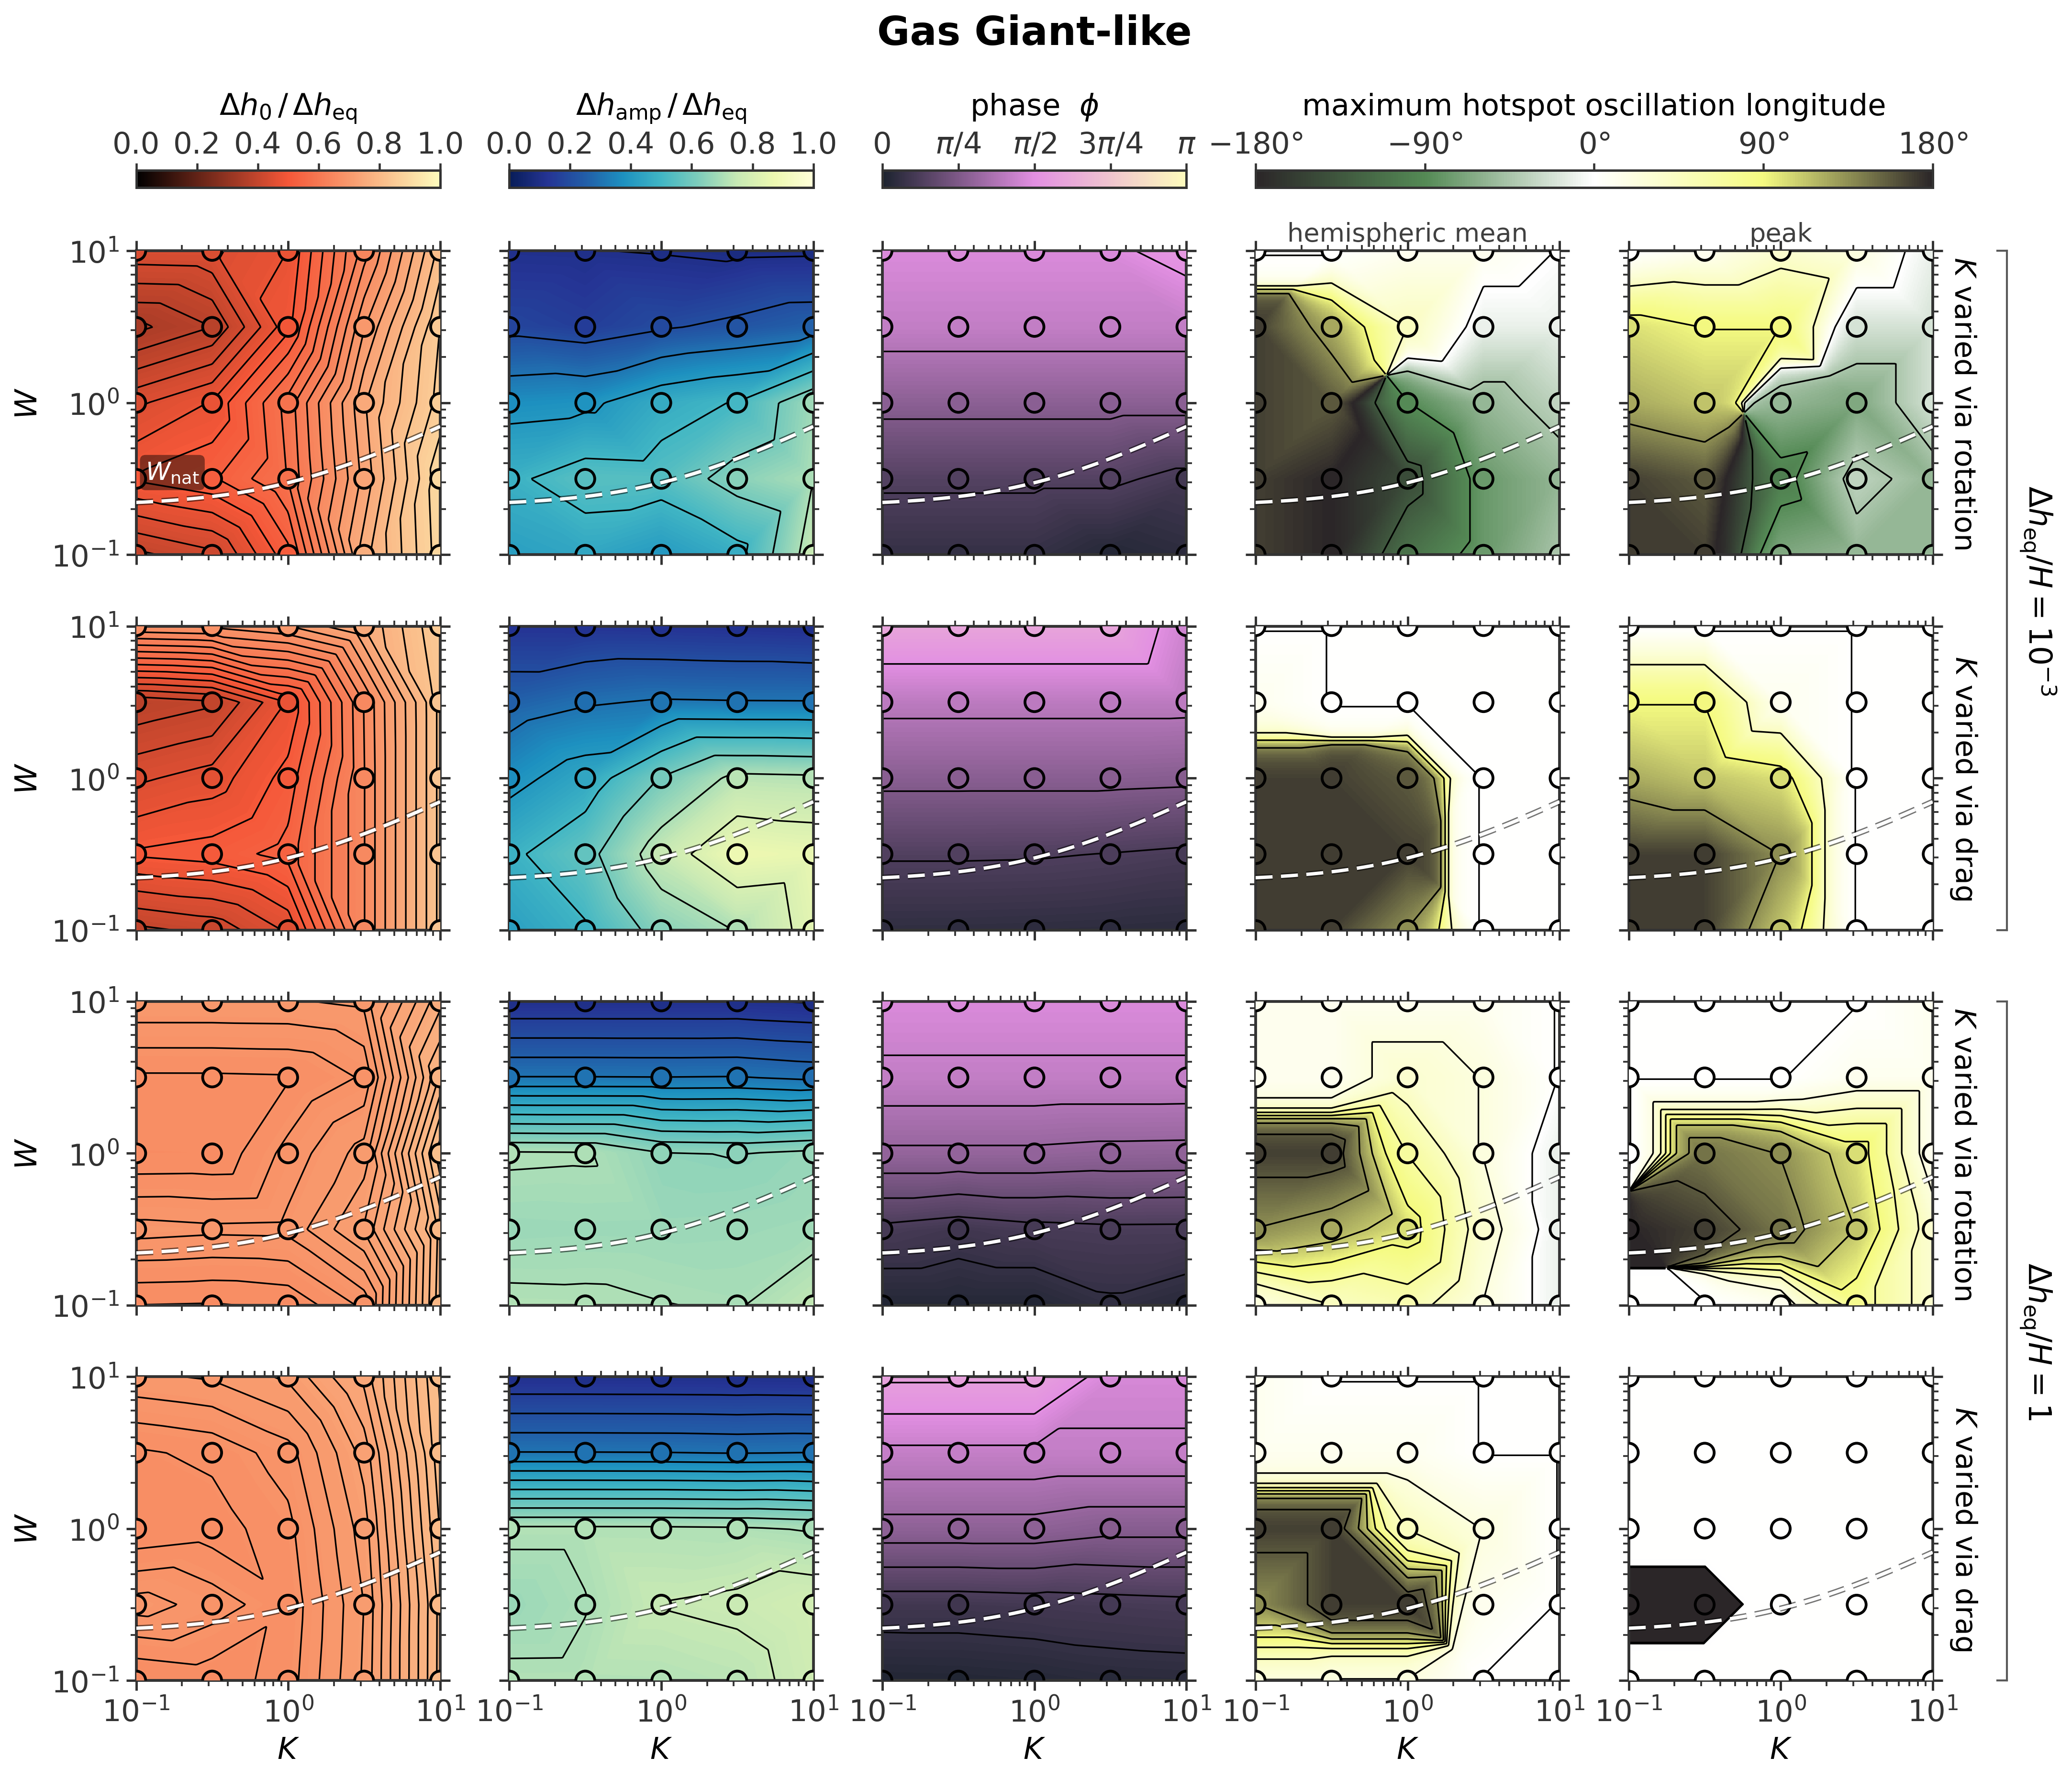
\includegraphics[width=\linewidth]{fig5_sim_gasgiantlike.png}
    \caption{Suite of simulation results for an tidally-locked gas giant planet, with the same quantities as in Figure \ref{fig:earth_analog}. Again, the theoretical results capture the dominant features in the simulations including the second order resonance effects. The magnitude plots still feature a local maxima in frequency corresponding to the location of the resonance which unseen in the theoretical results. Here, the differences between $\Delta h_{\rm eq} = 10^{-3} \times H$ and $1 \times H$ are stark and can be observed in most quantities presented. Notably different is the loss of westward (negative) hotspot oscillations in the strongly nonlinear regime with $\Delta h_{\rm eq} = 1 H$ for cases with varying rotation (compare column 4, rows 1 and 3).}
    \label{fig:hot_Jupiter}
\end{figure*}

% In this section we present results for a typical tidally-locked Earth-analog. For all the simulations, the following values are kept constant: $g = 9.81 \text{ m/s}^{-2}, a = 6400 \text{ Km}, H = 2 \text{ Km and } \tau_{\rm rad} = 10 \text{ days}$. Based on the above, the wave timescale comes out to be 5.28 days. This gives a $X$ value of 0.528. $\tau_{\rm drag}$ is varied between 0.28 and 55.9 days keeping a slow rotation period of 351 days. Rotation period is varied from 1.76 to 351 days, keeping the drag timescale constant at 55.9 days. For these set of parameters, the systems are mostly in the linear regime, except close to $K=0.1$ where the momentum equation looses linearity when $\Delta h_{\rm eq}= 1 \times H$; see blue line in Figure \ref{fig:lin_nonlin_lim}.
In this section we present results for the Earth-analog parameter set (Scenario A, Table~1; $g=9.81\,\mathrm{m\,s^{-2}}$, $a=6400\,\mathrm{km}$, $H=100\,\mathrm{m}$, $\tau_{\rm rad}=5\,\mathrm{days}$, $\tau_{\rm wave}=2.365\,\mathrm{days}$, $X=0.473$), which spans the linear regime for most of the $K$--$W$ space explored, with the exception of the lowest $K$ cases at $\Delta h_{\rm eq} = H$; see figure~\ref{fig:regime_constrast}(a). 

Figure \ref{fig:earth_analog} shows the simulated planetary responses for the above set. The general trends match the theoretical results. It has been shown previously for 3D atmospheres that if we break the global flow into divergent and rotational components via Helmholtz decomposition and evaluate their individual contributions to heat redistribution, we find that the divergent component carries most of the heat \cite{hammond2021rotational}. The same can be shown for the 2D shallow water model by replacing entropy $s$ in \cite{hammond2021rotational} by height $h$. The assumption of pure substellar to antistellar point flow, which is effectively only the divergent part of the flow captured by the linear theory thus is sufficient to produce the correct trends for planetary response. Additionally, the region of resonance occurring at low $K$ shows a local maxima at $W=2\sim1/0.473$, close to the white dashed line corresponding to the theoretical prediction of the resonance. We also see the constant part of the response to have a manifestation of the resonance effect; {\color{blue} this is not captured by any of the linearized theories and possibly is due to higher order wave mean-flow interactions}. 

An interesting phenomena is observed for some of the simulations when we track the location of the hotspot. The hotspot oscillates as it moves away from the substellar point towards the antistellar point and back proceeding from the \textit{eastward} direction, leading to thermal variability not only in time, but also in space. When it happens, we find the hotspot to be oscillating at the forcing frequency. The maximum amplitude of the hotspot oscillation is plotted in the last column of Figure \ref{fig:earth_analog}. The oscillation is seen to correspond to the region of the $K-W$ parameter space where the second-order theory predicts the resonant maximization of temporal variability. This is expected from the damped oscillator model of the planetary response, even though this phenomena is a spatially varying one.

The primary difference between the cases with changing drag and rotation is also apparent in these plots. Both set systems show spatial amplitude maximization during the resonance. However, it is only the cases with changing rotation period that also feature \textit{westward} oscillations. This behaviour is novel and is a key component of atmospheric variability for such planets, and will be investigated in detail in a later section.


\subsubsection{Typical gas giants}
\label{sec:hot_jupiter}

% In this section we present results for a typical tidally-locked gas giant with parameters from \cite{perez2013atmospheric}. For all the simulations, the following values are kept constant: $g = 10 \text{ m/s}^{-2}, a = 82000 \text{ Km}, H = 400 \text{ Km and } \tau_{\rm rad} = 0.1 \text{ days}$. Based on the above, the wave timescale comes out to be 0.3 days, which is much faster than the Earth-analog. Even the radiative timescale is significantly shorter. However, their ratio gives a higher value of $X=3$, larger than the first set for which $X=0.528$. $\tau_{\rm drag}$ is varied between 0.22 and 45.04 days keeping a slow rotation period of 282 days. Rotation period is varied from 1.42 to 282 days, keeping the drag timescale constant at 45.04 days. Note that the rotation rate exploration goes way beyond the realm of hot Jupiters, but these cases are included for completeness. For these set of parameters, only the momentum equation is nonlinear when $\Delta h_{\rm eq}$ is $1 \times H$, everything else is not. While effectively similar to the cases shown before, the degree of nonlinearity is much stronger; compare blue and red lines in Figure \ref{fig:lin_nonlin_lim}. The continuity equation is always linear.
In this section we present results for the gas giant parameter set (Scenario B, Table~1; $g=10\,\mathrm{m\,s^{-2}}$, $a=82{,}000\,\mathrm{km}$, $H=4\times10^{5}\,\mathrm{m}$, $\tau_{\rm rad}=0.1\,\mathrm{days}$, $\tau_{\rm wave}=0.4745\,\mathrm{days}$, $X=4.745$), taken from \cite{perez2013atmospheric}. Compared to the Earth-analog, $X=4.745$ implies a significantly higher $\tau_{\rm wave}/\tau_{\rm rad}$ ratio. The entire $K$--$W$ space is in the overdamped second-order regime, but the pseudo-resonance amplitude peak described above still appears near $W \approx 0.25$. Only the momentum linearity condition is violated at $\Delta h_{\rm eq} = H$; the continuity equation remains linear throughout (see red line in figure~\ref{fig:regime_constrast}(a). 

Figure \ref{fig:hot_Jupiter} shows the planetary response to variable irradiation for the set of gas giant planets described above. Comparing with the theoretical plots corresponding $X=4.75$, we find a good match with both the first and second-order theories. The resonant frequency has now moved down to a smaller value of approximately $W=0.2\sim 1/4.75$ obeying the $1/X$ rule from theoretical predictions in \S \ref{sec:in_dam_resp}. The top two rows, for which $\Delta h_{\rm eq}$ is $10^{-3} \times H$, are in the linear regime, while the bottom two are not. As expected, the linear simulations match the theory better--- for the bottom rows, the $\Delta h_{\rm o} / \Delta h_{\rm eq}$ plots have more averaged out values over the $K-W$ parameter space, although the contour lines show that the fundamental structure is preserved. This is because, several of our assumptions breakdown in nonlinear spherical simulations as mentioned in \S \ref{sec:assu_lim}, and additional physics like wave-mean flow interactions come in. This is also seen in the amplitude plots with values averaged out for low $W$ values.   

We also observe that the phase offset goes beyond 90$^\circ$, but never too far beyond to 180$^\circ$ as is determined from the second order theory. \citep{Shamir2023} shows that the steady, linearized Matsuno--Gill solution is only strictly valid when the temporal variation of the forcing is slow compared to the radiative/frictional relaxation time of the atmosphere -- a requirement that traces back to the original steady-state assumption of \citet{Matsuno1966} and \citet{Gill1980}. We notice an analogous effect in our simulations: at high instellation-oscillation frequency, the planetary response deviates from the purely sinusoidal form of the forcing towards more complicated forms (not shown here), even in nominally linear-amplitude runs. This likely leads to higher-order dynamics which prevents the phase lag of the planetary response at high instellation-variation frequency from reaching the theoretical maxima of $180^{\circ}$ even in the otherwise-linear regime. The effects of nonlinearity by its intrinsic virtue is at multiple spatial and temporal scales, and hence the nonlinearity conditions in equations~\eqref{eq:lin_condt1}--\eqref{eq:lin_condt2} may be regarded as sufficient, but not the only, conditions for nonlinear behaviour to emerge. Regardless, the large-scale flow and height patterns are still dominated by the linearized dynamics. 

Finally, hotspot oscillations that appear in the resonant region are dominated by purely eastward movement in the nonlinear regime. The change can be seen comparing column 4 panels in rows 1 and 3. Westward oscillations still appear in at low forcing strengths as it is in the linear regime. This is different from what we have seen before and explained in detail in a latter section. Overall, our simulations across Earth-analog and gas giant parameter regimes demonstrate good agreement with theoretical predictions; showing that the drag and rotation contribute similarly to the response and hence combining them into the effective drag term is not a poor assumption. Linear regime simulations match theory more closely than nonlinear regimes, as expected. Despite their degenerate effect on the leading order response, we also find that changing rotation and drag affect the time varying location of the planet's hotspot in different ways. The hotspot location is a key component affecting observational signatures of such planets and we deliberate on their nature in the next section.


\section{Global atmospheric variability}
\label{sec:discussion}

In this section we delineate the imprint of varying irradiation on the atmospheric variability of a planet, specifically focusing on westward and eastward hotspot oscillations and probing the underlying mechanisms in the switch of this behaviour in linear and nonlinear regimes. 

{\color{red}Add literature for hotspot oscillations and contrast MHD with HD.}

\subsection{Hotspot oscillations}

As seen previously in Figure \ref{fig:earth_analog} and \ref{fig:hot_Jupiter}, the direction and extent of hotspot oscillations depend on both the rotation rate and the drag timescale, even though the other theoretically derived response parameters such as magnitude, amplitude and phase-lag are agnostic to these variables. For slowly rotating Earth-like and gas giant-like drag-varying batches, hotspot oscillations are purely eastward across all drag values. The extent of oscillation varies over the $K$--$W$ parameter space with the maximum longitudinal shift (180 degrees) occuring at the location of the resonance and decaying in all other directions. Higher drag values lead to smaller oscillations, albeit justified by the dissipative nature of drag on wave or advection driven dynamics. The positive correlation between the maximum hotspot oscillation and the maximum planetary response amplitude at the resonance in the $K$--$W$ parameter space shows that the phenomena are connected, with the former likely also causing the latter. We expect this because both the resonance and hotspot oscillations result from inertial physics of the system. 

When rotation is varied, we find hotspot oscillations to be eastward at slow rotation and westward at fast rotation, with the maximum magnitude of oscillation still occuring at the resonance, for the Earth-like cases. Note here that this is primarily linear system. In most cases, the hotspot oscillates on only one side of the substellar point. However, in some cases, especially close to the transition rotation rate, the hotspot oscillates across the substellar point both westward and eastward. In Figures \ref{fig:earth_analog} and \ref{fig:hot_Jupiter}, such cases are still represented by the maximum hotspot oscillation thereby omitting this information, but the actual complex hotspot oscillation is better visualized in Hovmöller diagrams {\color{red} (cite?)} shown hereafter (Figure~\ref{fig:hovmoller}).  

Finally, for the gas giant cases in the nonlinear regime ($\Delta h_{\rm eq} = H$), we find that the oscillations are eastward even at fast rotation rates, making the behaviour consistent across the entire parameter space. This is a qualitative departure from linear behaviour and should have direct implications for observable phase curves for different planets as discussed in Section~\ref{sec:phase_curves}.

To visualise how rotation and nonlinearities alter the hotspot dynamics and track its movement, we construct Hovmöller diagrams — longitude--time maps of the height field — for the three representative linear and nonlinear gas giant cases with changing rotation. Figure~\ref{fig:hovmoller} compares linear ($\Delta h_{\rm eq} = 10^{-3}H$) and nonlinear ($\Delta h_{\rm eq} = H$) runs at three rotation periods (282.9, 14.9, and 1.42 days), showing the last three forcing cycles of each simulation. Two diagnostics are overlaid on every panel that show the meridional mean height averaged in \textit{a window of 90 degrees width about the equator}, the hemispheric average height and their corresponding normalized values in order: the location of maximum height or the hotspot (white solid line) and the hemispheric-maximum hotspot (black dashed line). The dotted green line marks the substellar longitude. Note that the hemispheric average hotspot does not follow the same path as the meridional mean hotspot because they are different forms of averaging applied to the same height field. The latter is a better indicator of the observable hotspot position owing to its projected face average (see Figure \ref{fig:schem_hemi}). 

The first thing to note is that the planetary response is strongly modulated by the instellation in all cases. This is due to the short radiative timescale of the gas giant parameter set of 0.1 days. Second, the normalization carried out for each individual timestep and it highlights the instantaneous height maxima helping visualize the hotspot location. The absolute hotspot location matches well the maxima of the normalized meridional mean height, while the hemispheric-mximum hotspot matches the normalized hemispheric average height. Finally, the same conclusions are drawn from the Hovmöller diagrams as from the hotspot oscillation plots in Figures~\ref{fig:earth_analog} and \ref{fig:hot_Jupiter}: linear cases show a transition from eastward to westward hotspot oscillations with increasing rotation, the extent of oscillation decreasing with rotation, while nonlinear cases remain eastward across all rotation rates. 


\subsection{Role of rotation} \label{sec:role_of_rotation}

From the simulation results above, we note that the reflection of the resonance on the height response amplitude is rather minimal, but the hotspot oscillation is a more sensitive indicator. The resonance, if significant, always occurs at small values of rotation and drag (left hand side of the $K$--$W$ plane). From linearized theory we know that strong rotation inhibits the transport of heat from the day to the night side via waves (see also simulations of \citealp{Tan2020}), and so does strong drag. It is thus expected that the resonance and consequently hotspot oscillations will be the strongest when the wave propagation is least inhibited.

\begin{figure*}
    \centering
    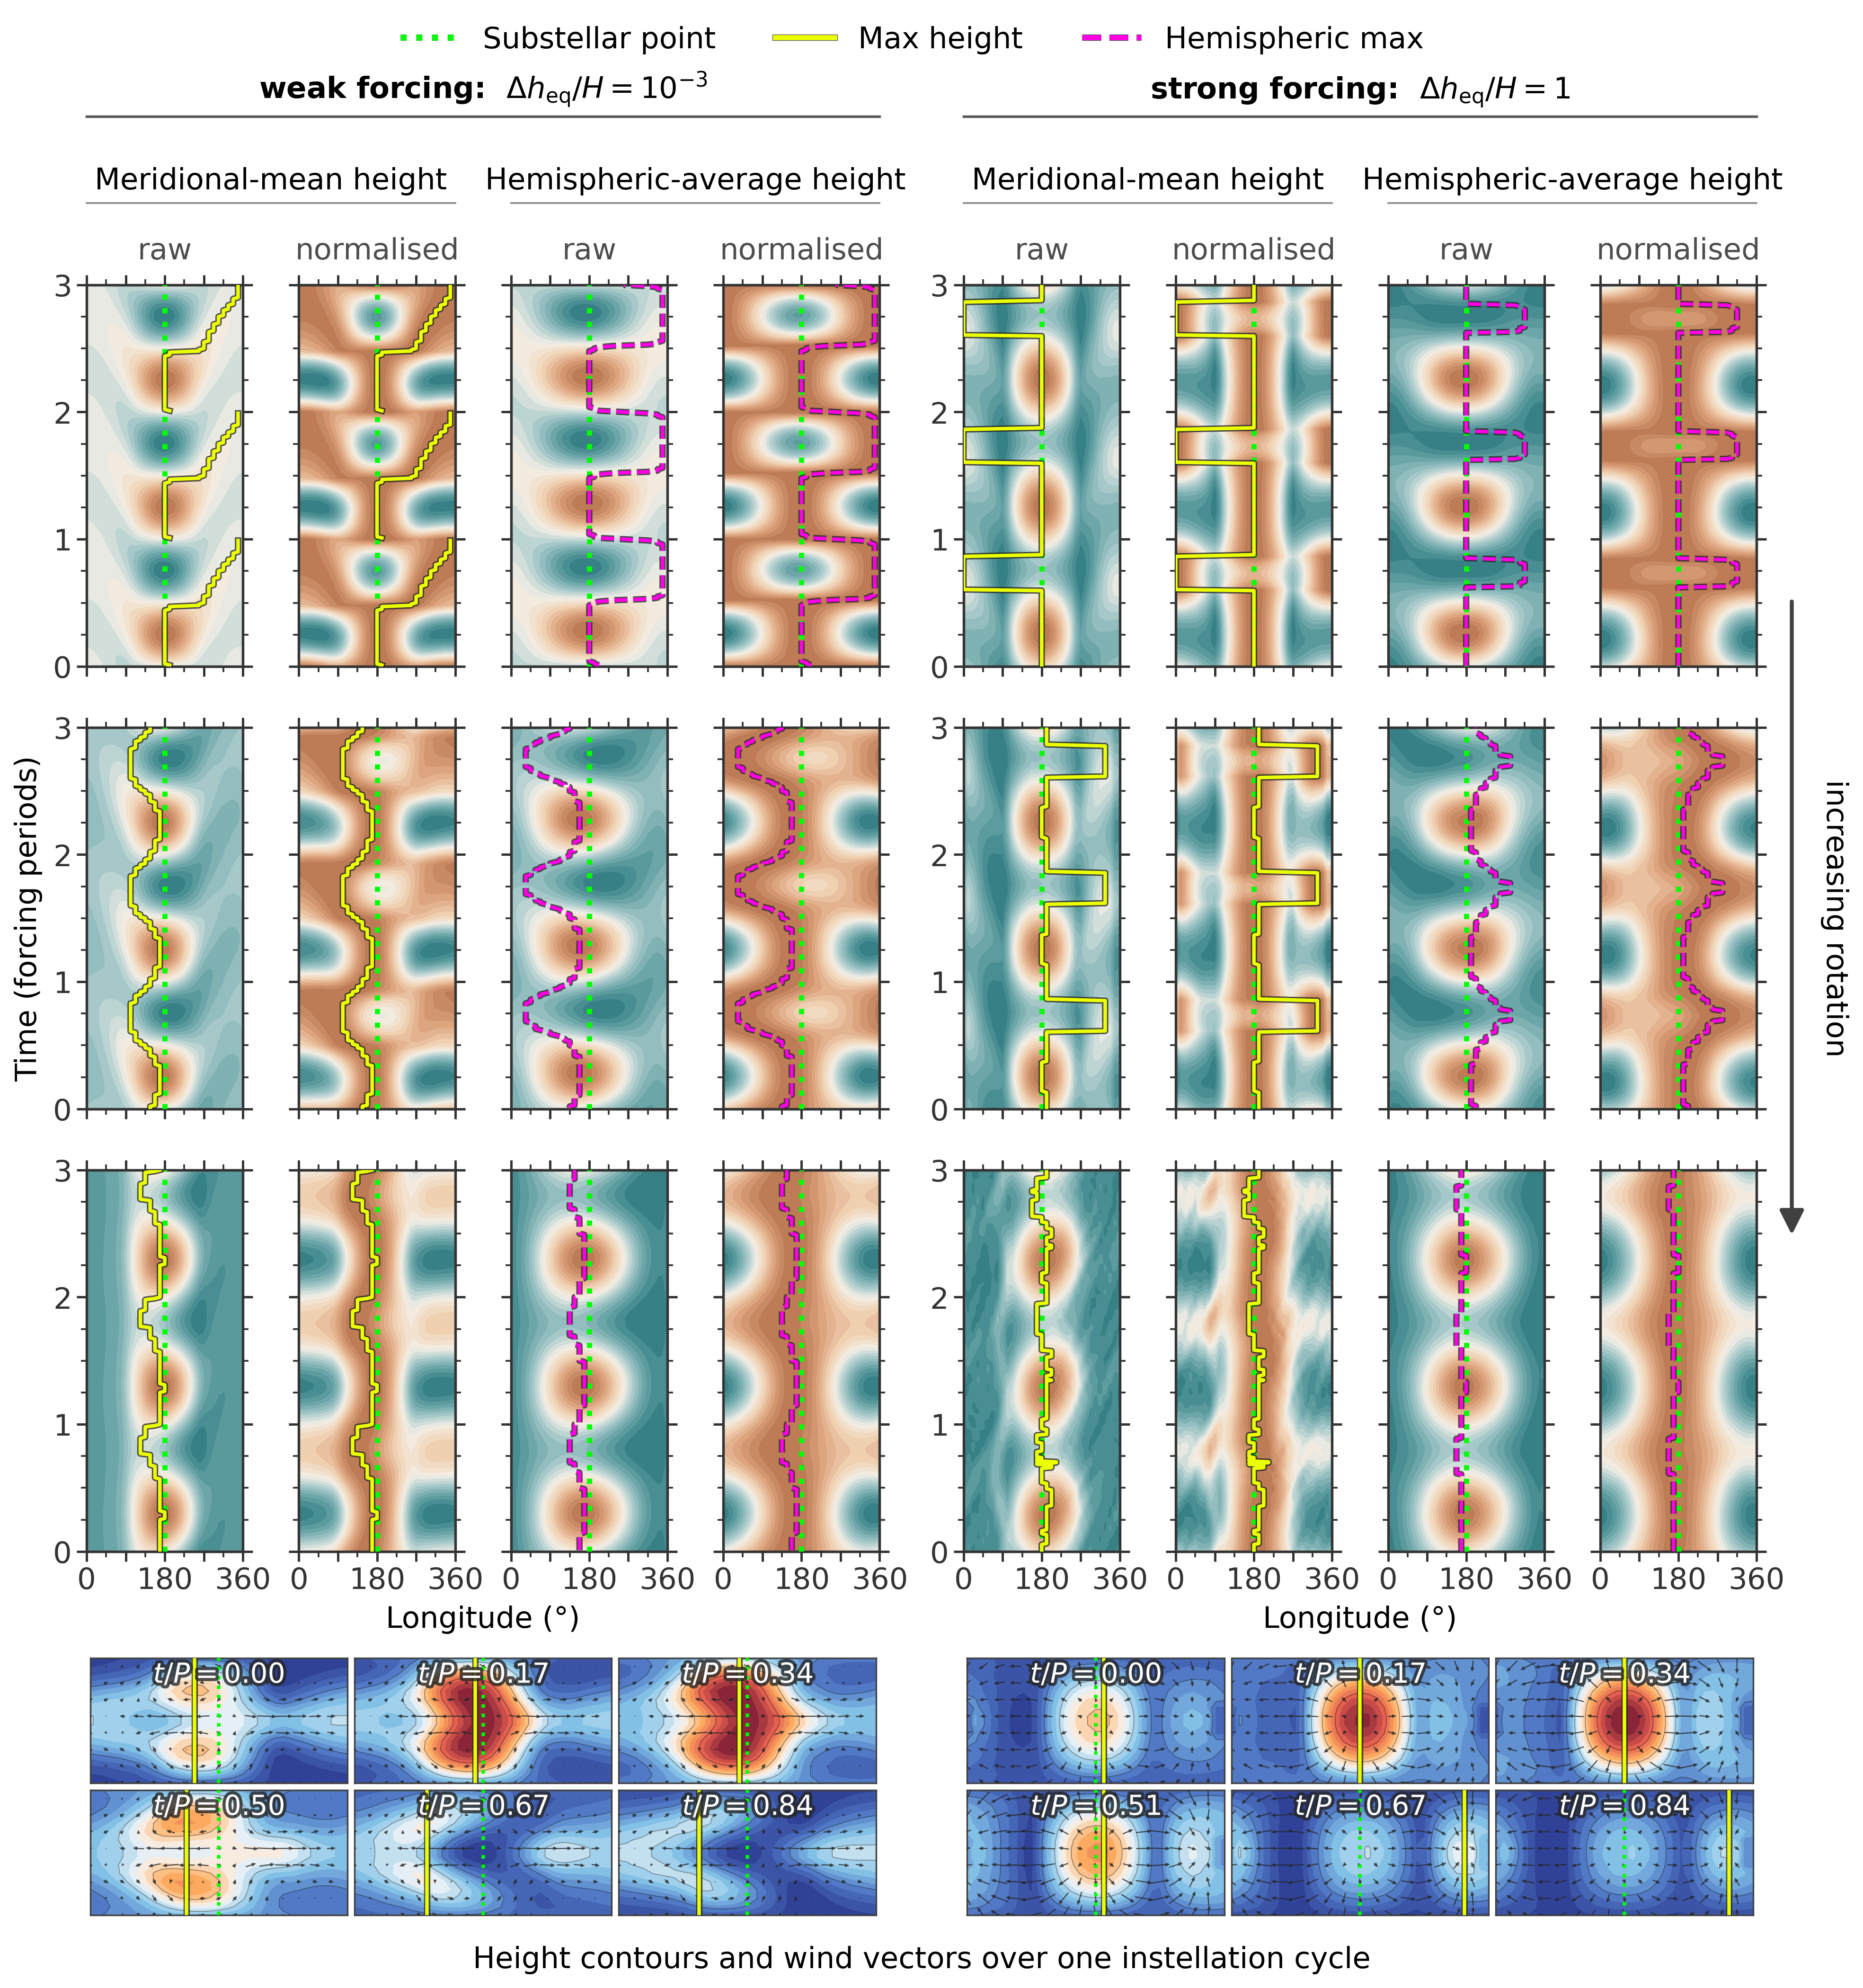
\includegraphics[width=\linewidth]{hovmoller_lin_vs_nonlin.png}
    \caption{Hovmöller diagrams or timeseries of hotspot location relative to background zonal height profiles for six gas giant planets showing hotspot oscillations switching from westward to eastward with rotation as the system transitions from linear to nonlinear regime. The left column corresponds to $\Delta h_{\rm eq} = 0.001$ and the second column to $\Delta h_{\rm eq} = 1$. Each row represents an increasing rotation period (282.9, 14.9 and 1.42 days), and columns show different diagnostic quantities: the meridional mean height, the merdional mean height normalized by the max height at each timestep to expose the instantaneous hotspot location, the hemispheric average height, and similarly normalized hemispheric average. The dotted green line marks the substellar longitude. The colorbars for background height fields are dropped to keep the Figure clean focussing on the hotspot locations. White solid lines track the meridional mean-height hotspot, while black dashed lines track the hemispheric-maximum hotspot. The time window shown spans the last ~3 forcing periods of the respective simulations.}
    \label{fig:hovmoller}
\end{figure*}

To understand the role of rotation let us consider slow rotation with \textit{constant} instellation first. In this case, the day-night radiative forcing creates a standing equatorial Kelvin wave pattern, akin to the gravest gravity wave mode, that closely resembles the equilibrium height field but is not the same \citep{Gill1980,ShowmanPolvani2011}. Since the Kelvin wave has an eastward propagating phase velocity, on varying the instellation, the system responds to the forcing by letting the Kelvin mode travel eastward till the instellation comes back to a maxima. Thus the point of maximum height, the hotspot, travels eastward and gets reset to the substellar point towards the end of the forcing cycle; see Figure \ref{fig:hovmoller}, white line in the top left panels. The slowest rotation case is extremely close to the non-rotating case, where gravity wave propagation is isotropic from the substellar to the antistellar point. This is why we see the height fields to be almost symmetric about the substellar point even though the hotspot oscillation points to the east as a result of the eastward propagating weak Kelvin wave mode being excited by the instellation forcing.

As the rotation rate is increased (second and third rows of the left hand side panels of Figure \ref{fig:hovmoller} representing the linear regime), the Coriolis force becomes stronger. This leades to another off-equatorial wave mode, the Rossby wave, to be excited. The height fields are more asymmetric with the height maxima to the west of the substellar point (see second panel). The Rossby wave mode is westward propagating \citep{Matsuno1966,Gill1980} and may justify the westward oscillation observed at fast rotation rates. However, in principle, both the Kelvin and Rossby waves are excited at all rotation rates according to linearized $\beta$-plane theory \citep{Matsuno1966,Gill1980}. Changing $\Omega$ on the $\beta$-plane only rescales the two wave solution in space and time — it does not change the relative amplitude of Kelvin vs. Rossby wave content, because that ratio is fixed by the forcing shape and damping alone in the scaled coordinates. Moreover, our system is on a sphere similar to the system in \cite{Shamir2023}. In their linearized case, even more fundamental wave modes like the eastward and westward inertio-gravity waves (EIG, WIG) and the mixed Rossby--gravity (MRG) wave are shown to be present. Each of these modes have their own direction of propagation and are excited at different degrees by the nature of forcing imposed, which is different between their study and ours. Additionally, even though we find that height contrast is agnostic to rotation and drag, \citet{Shamir2023} shows the wave mode decomposition is differently sensitive to these quantities and hence affects the hotspot location. Reducing rotation rate progressively breaks the two-wave (Kelvin+Rossby) picture altogether, enhancing the inertio-gravity modes that are not fully captured by the pure equatorial $\beta$-plane theory. The exact mechanism for the switch in direction of hotspot oscillation is thus not clear and will be investigated in a future study.


\subsection{Role of nonlinearities}
\label{sec:role_of_nonlinearities}

We now study the role of nonlinearities, the conditions for which are given in equations~\eqref{eq:lin_condt1} and~\eqref{eq:lin_condt2}. Simulations representing the nonlinear gas giant regime ($\Delta h_{\rm eq} = H$) are based on these conditions. However, the conditions themselves are agnostic to the forcing frequency. We have noted that a high forcing frequency can play a role in the local rise of nonlinearities, but we do not resolve small scales here and hence the nonlinear behaviour is restricted to its effect on the global scale features. We emphasize that nonlinear behaviour is not synonymous with wave-driven behaviour, even though both formally arise from the same inertial terms in the momentum equations.

In the nonlinear regime at low rotation (first row, right-hand-side panels of Figure~\ref{fig:hovmoller}), we see the onset of a switching behaviour of the hotspot between the substellar and antistellar points, in contrast to the gradual eastward drift seen in the corresponding linear simulations. This hints at the presence of higher-order interactions that are absent in the linear regime \citep{ShowmanPolvani2010,ShowmanPolvani2011}. The exact mechanism responsible is not yet clear and warrants further investigation. However, the hotspot still oscillates eastward in this regime, similar to the linear case.

At intermediate rotation (2nd row, right-hand-side panels), the hotspot oscillations continue to occur in the eastward direction, in contrast to the westward oscillation seen in the corresponding linear case. We suggest that the suppression of westward oscillations in the nonlinear regime is a consequence of the wave-mean-flow interaction mechanism of \citet{ShowmanPolvani2010,ShowmanPolvani2011}. In that mechanism, the equatorward eddy momentum flux convergence associated with the standing Kelvin--Rossby wave pattern spins up a persistent eastward equatorial superrotating jet. Once established, this jet Doppler-shifts the stationary forced wave pattern to produce an eastward hotspot offset in the absence of instellation variation \citep{HammondPierrehumbert2018}. In the linear regime, by contrast, the wave-driven momentum flux convergence scales weakens and is unable to spin up or maintain an equatorial jet against drag. Without a jet to Doppler-shift the wave pattern, the Rossby-eddy pattern is free to dominate at fast rotation, producing the westward oscillations described above. We note, following \citet{Nicolas2026}, that the strength of superrotation and the magnitude/direction of the resulting hotspot offset are not related in a simple, one-to-one way, but are jointly controlled by rotation, drag, and radiative timescale; the argument above should therefore be regarded as a plausible leading-order mechanism rather than a complete explanation.

Finally, at high rotation rates (3rd row, right-hand-side panels), the hotspot offset -- while still eastward -- is reduced, as rotation inhibits the day-to-nightside transfer of heat, similar to the 3D GCM simulations of \citet{Tan2020}, who also find the eastward offset to shrink as rotation increases.

\subsection{Caveats and further exploration}

The interpretation above rests on a qualitative argument for how wave--mean-flow interactions might suppress the westward, Rossby-dominated pattern found in the linear regime, but we have not yet directly diagnosed the jet or decomposed the flow into its constituent wave modes. Two directions of investigation would sharpen this picture considerably. First, an explicit projection of both the linear and nonlinear solutions onto the free wave modes of the system, following the methodology of \citet{Shamir2023}, would let us test directly the mechanism of hotspot behaviour in the linear regime. Second, in the nonlinear regime, we may probe through a time-dependent helmholtz decomposition of the flow field \citep{hammond2021rotational}, the contributions of the divergent, eddy-rotational and eddy-mean components and the timescales over which they grow and decay subject to transient instellation to better understand how the equatorial jet spins up and equilibrates \citep{ShowmanPolvani2011} thereby delineating the hotspot behaviour. Disentangling the transient jet dynamics from the quasi-steady wave response is left for future work.

\section{Observational implications}

\subsection{Synthetic phase curves}
\label{sec:phase_curves}

\begin{figure*}
    \centering
    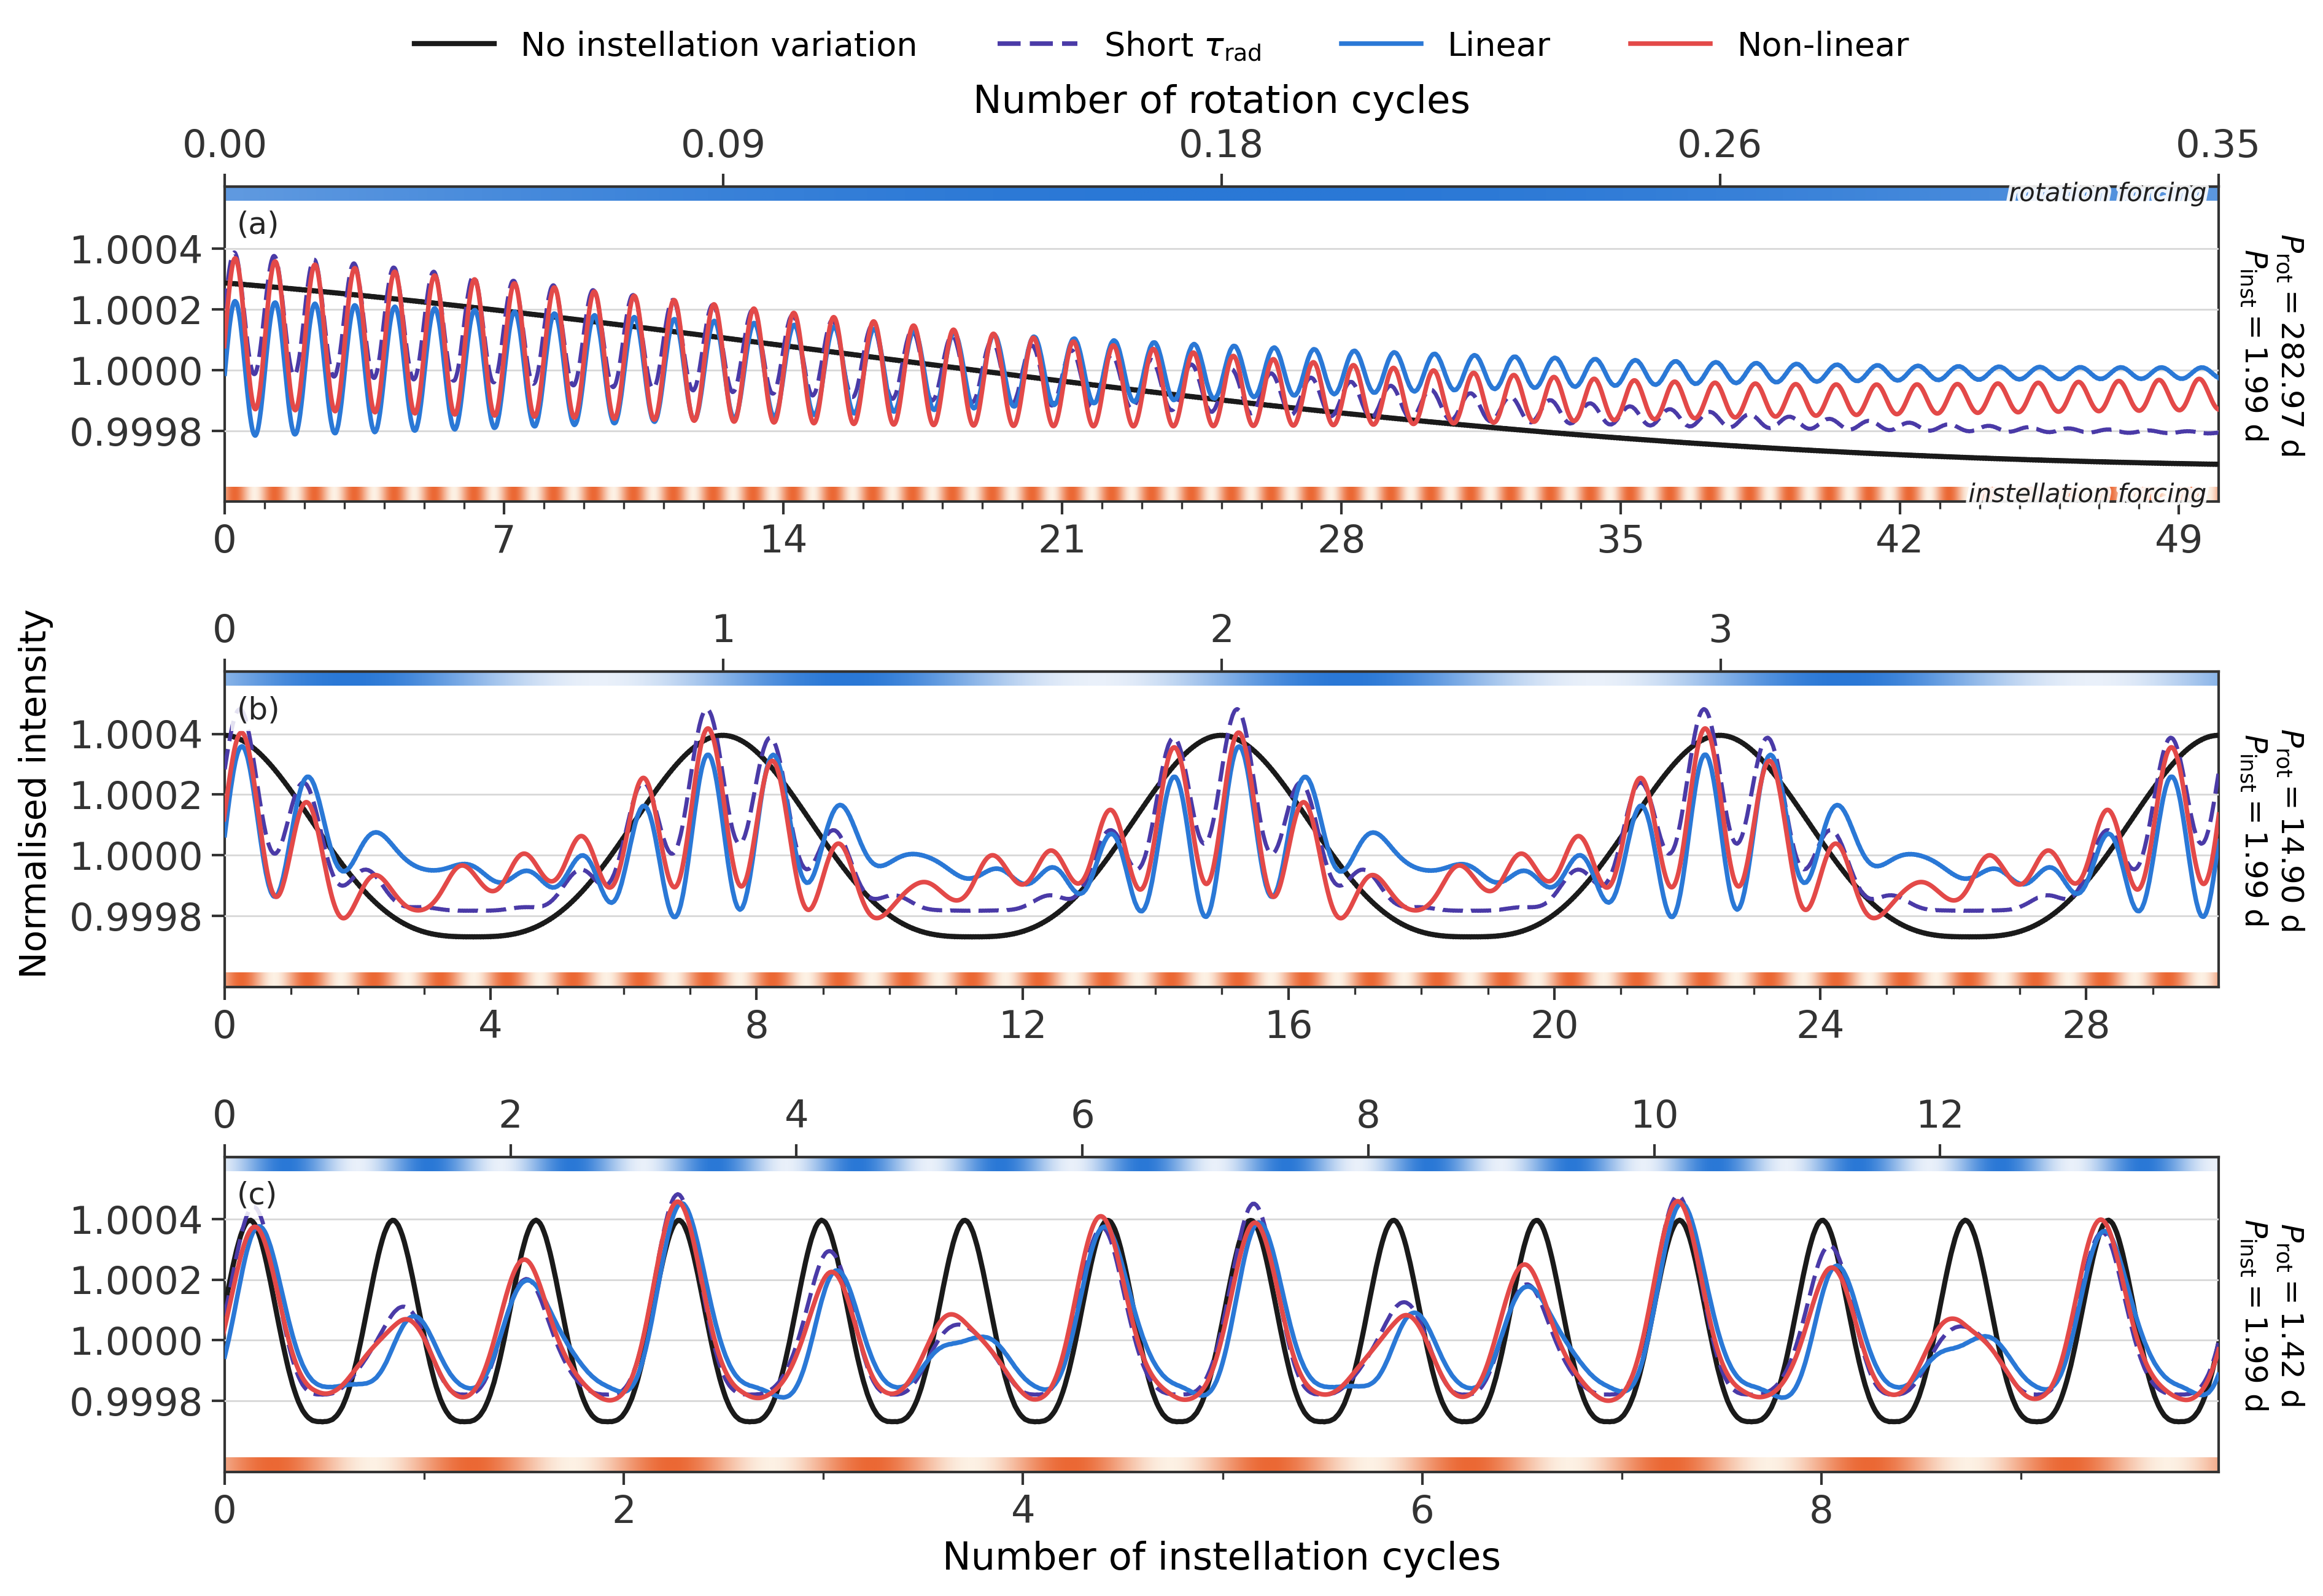
\includegraphics[width=\linewidth]{phase_curves.png}
    \caption{Phase curves for the same rotation periods as in Figure \ref{fig:hovmoller} with linear and nonlinear cases show significant differences. Each panel shows four normalized phase curves: case for no instellation variation, or simply the phase curve of the forcing profile (black); the same with instellation variation (purple); the linear case (green); and the nonlinear case (red). The background contours represent instellation variations (yellow-red, lower half) and rotation variations (blue and white, upper half) with corresponding cycle number on the top and bottom axes.}
    \label{fig:phase_curve}
\end{figure*}

The disc-integrated flux — the observable phase curve — is constructed by integrating the hemispheric-averaged height field over the visible hemisphere as a function of orbital phase. Figure~\ref{fig:phase_curve} shows phase curves for the same six rotation periods as the Hovmöller analysis. Each panel overlays four normalised curves: a baseline with no instellation variation (black); a constant-instellation run with orbital phase sampling (purple); the linear variability case (green); and the nonlinear variability case (red). Background shading encodes the instellation cycle number, allowing direct comparison of the forcing periodicity and the atmospheric response.


% {\color{teal} Phase curves simulated near the resonant $W_{\rm res}$ may contain multiple frequency components: the forcing frequency $\omega$, the natural frequency $\Omega_{\rm o}$, and their beat frequency $|\omega - \Omega_{\rm o}|$. A Fourier analysis of these phase curves would reveal this beating structure as a long-period modulation of the peak-to-trough amplitude, which would be a direct observational signature of the second-order wave dynamics.}

The first thing to note in Figure~\ref{fig:phase_curve} is that both the rotation and instellation variation modes crop up distinctly in the phase curves when the periods are significantly separated from each other as in the first two panels, as opposed to when they are similar as in the last panel. In this case, we find the overall variation to match the rotation better than the instellation variation, although the relative secondary eclipse heights is strongly modulated by the instantaneously available instellation; smaller peaks in yellow regions (low instellation) and larger peaks in red (strong instellation). Also, the eclipsing phase (lowest points) of the instellation variation cases never hits the lowest of the constant instellation case because the hotspot oscillations averaged over time help increase the nightside temperature. The highest point is consequently higher, although not observed as prominently for the fastest rotating planet. The reason the fastest planet shows a different behavior is probably because it is out of the resonance regime where the planet response is well characterized by the first-order linearly damped model in \S \ref{sec:first_order}.

The additional modulation of the phase curve introduced by instellation variability scales linearly with $F$, the fractional semi-amplitude. In the current work this value has been kept to 50$\%$ of the constant magnitude, which is not realistic for most systems. However, the qualitative behaviour of the phase curves is expected to remain similar. 

{\color{teal} Add JWST baseline comparison estimates.}


\subsection{Where do planets fall in $K$--$W$ space?}
\label{sec:kw_space}

\begin{figure*}
    \centering
    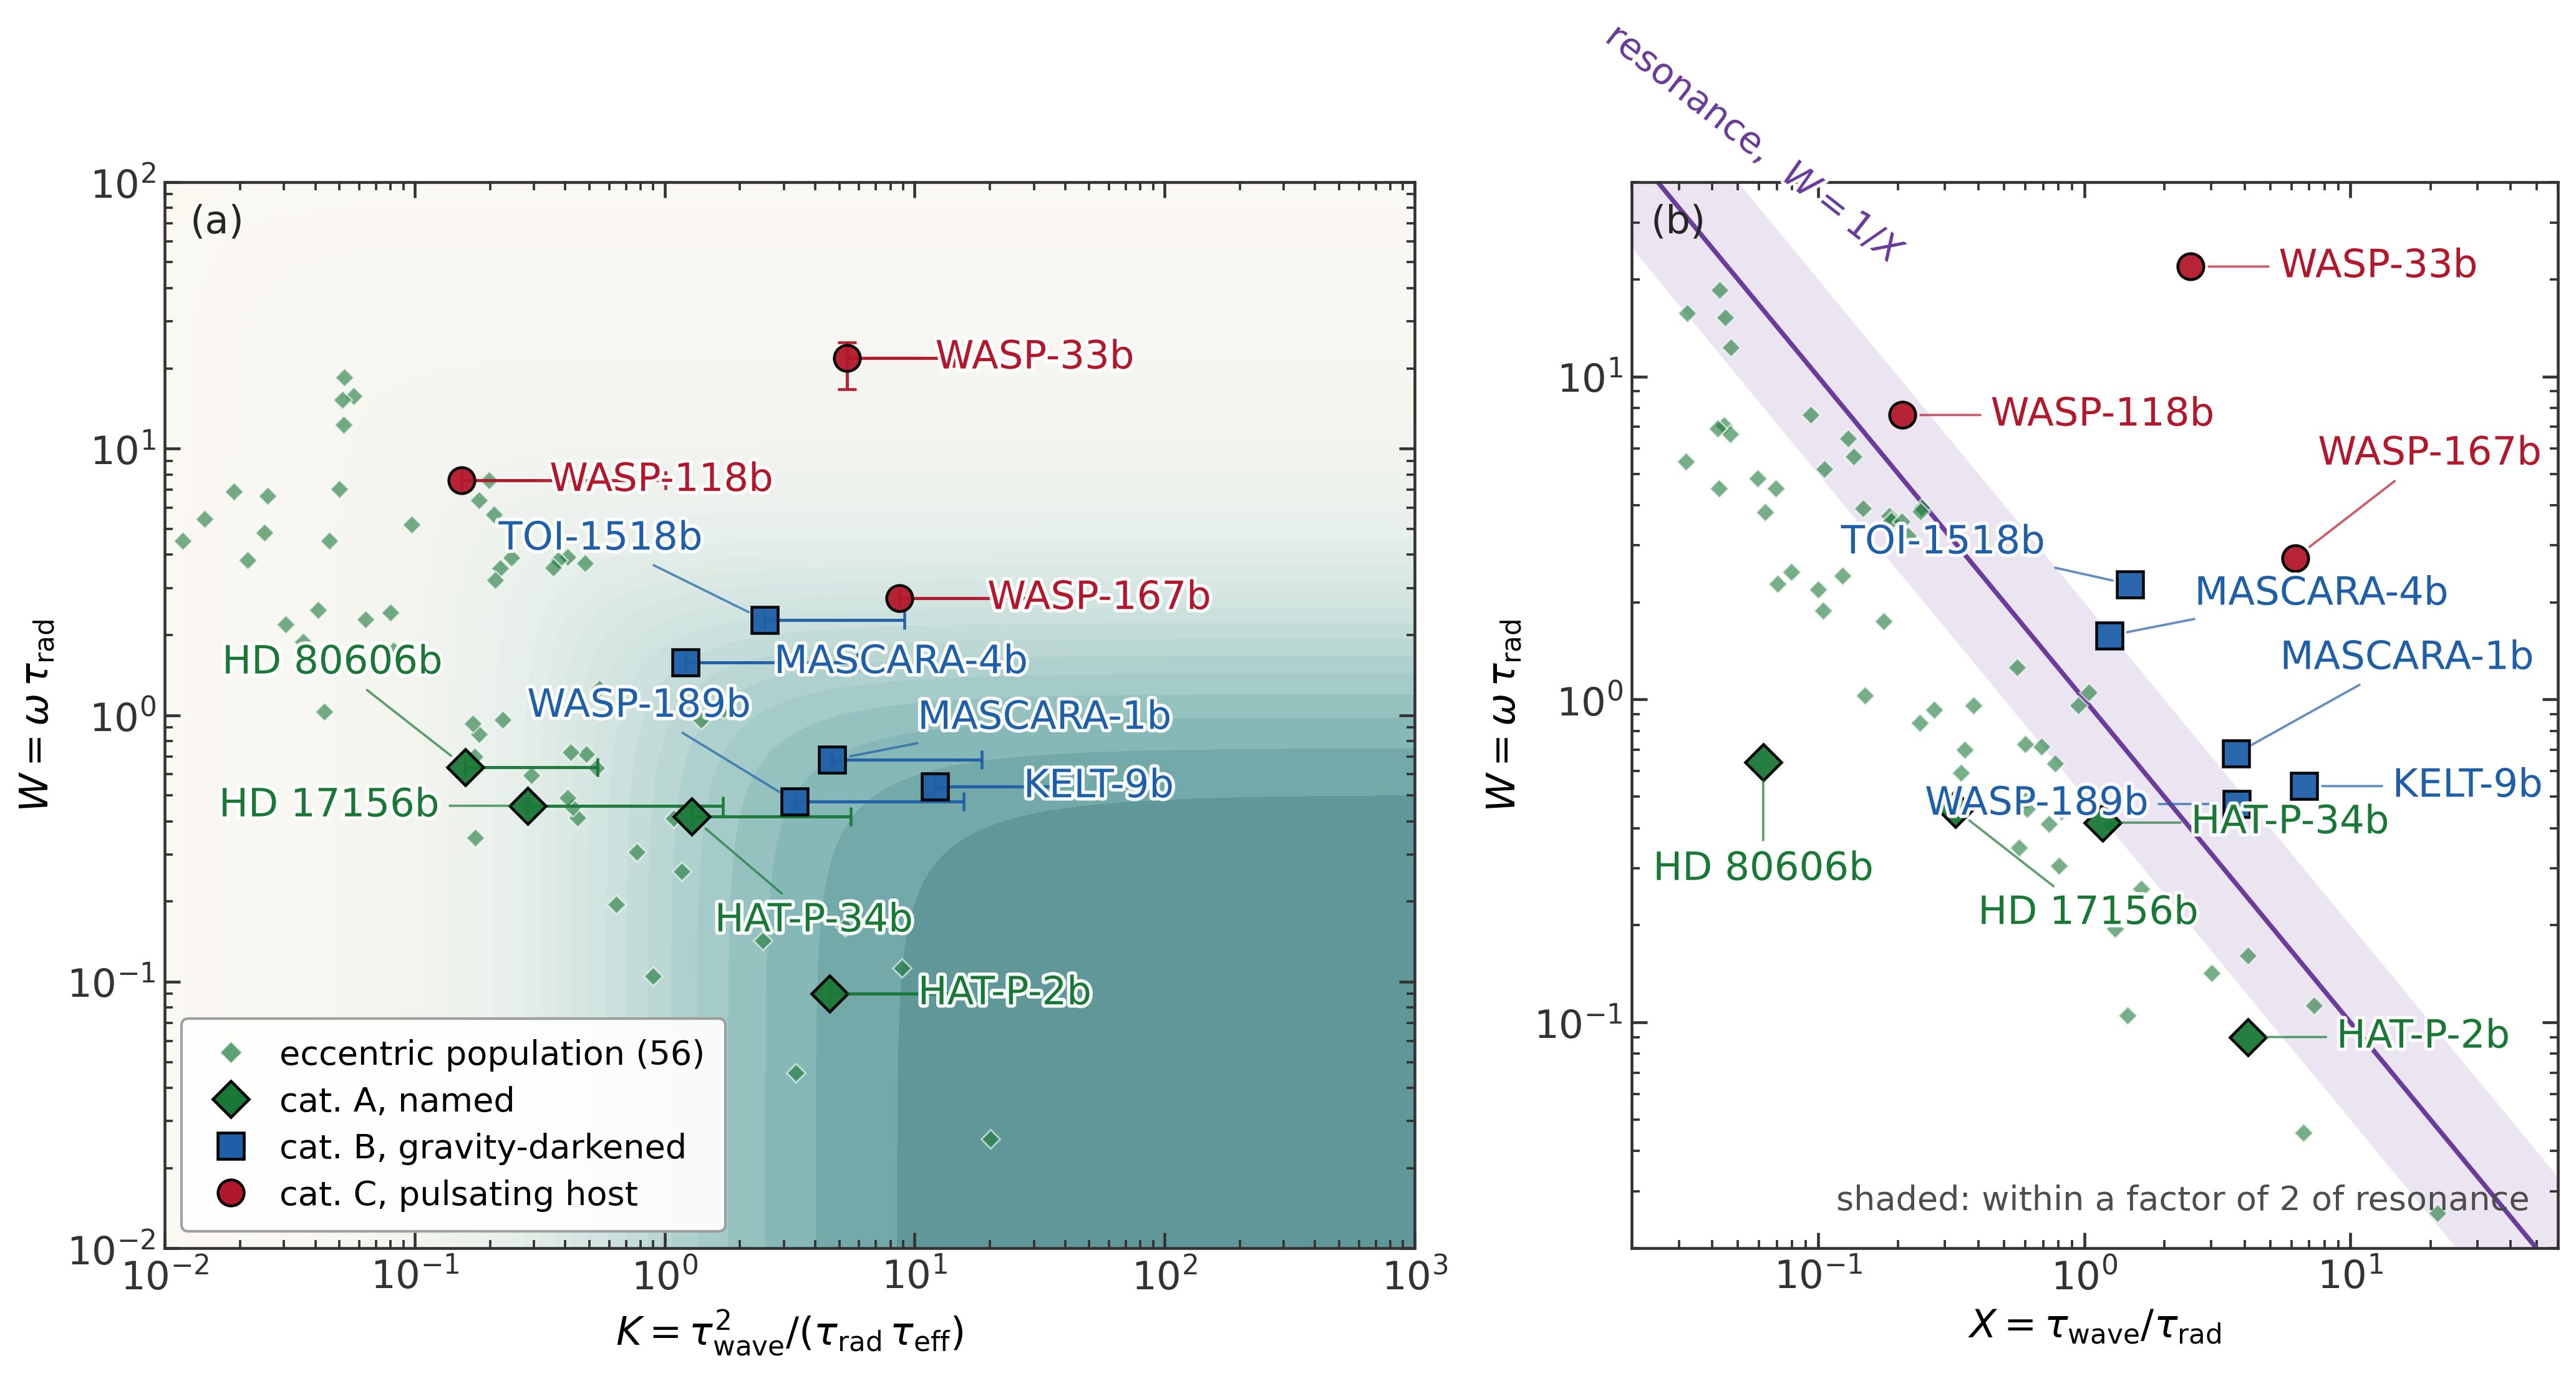
\includegraphics[width=\linewidth]{kw_planets.png}
    \caption{Sixty-eight variably irradiated systems placed in the $K$--$W$ plane (a) and the $W$--$X$ plane (b), with $K$, $W$ and $X$ computed for each from archival radii, temperatures and periods (Appendix~\ref{app:kw_calc}, Table~\ref{tab:kw_systems}). Marker shapes encode variability category: circles (C, pulsating host), squares (B, gravity-darkened host), diamonds (A, eccentric orbit); small diamonds are the eccentric population, large symbols the systems named in the text. (a) The shaded field is the first-order amplitude response $\left[(1+1/K)^2+W^2\right]^{-1/2}$, which is independent of $X$ and so applies to the whole sample at once, darker towards the strongly retaining, slowly forced corner; it carries no restoring force and hence no resonance of its own. Horizontal bars are one-sided, running from the drag-free $K$ at the marker to the strong-drag value at $\tau_{\rm drag} = 10^4$~s; the vertical bar on WASP-33b spans its host's pulsation spectrum. (b) Distance from resonance in frequency space. Resonance sits at $W = 1/X$, the purple line of slope $-1$; the shaded band marks the systems within a factor of two of it, $0.5 \le W/W_{\rm res} \le 2$ with $W_{\rm res} = 1/X$. Twenty-five of the sixty-eight systems fall inside it.}
    \label{fig:kw_planets}
\end{figure*}

In this section we place real systems on $K-W$ and $X-W$ spaces. The location on $K-W$ space tells us whether the planetary response to variable irradiation is muted or strong, and that on the $X-W$ space says whether or not they lie close to their corresponding resonances. Figure~\ref{fig:kw_planets} does this for sixty-eight systems spanning three variability categories --- eccentric orbits (A), gravity-darkened hosts (B) and pulsating hosts (C) --- using parameters computed from archival radii, temperatures and periods. The calculation, the sample selection and the per-system values are given in Appendix~\ref{app:kw_calc}; here we state only what the placements imply for observations.

Three features stand out. First, every system lies close to the $K = X$ boundary between the wave-active and drag-dominated regimes. In the drag-free limit the ratio is simply $K/X = \tau_{\rm wave}\Omega$, and it spans only $0.28$--$2.59$ across the whole sample, with a median of $0.88$. This is a generic property rather than a selection effect: tidally locked and pseudo-synchronous giants have $\tau_{\rm wave} \sim 0.3$--$0.7$~d and rotation periods of a few days, so $\tau_{\rm wave}\Omega$ cannot be far from unity. Observed close-in giants therefore populate the transition between the two dynamical regimes, and neither the inertial nor the overdamped limit may be applied to them safely.

Second, and consequently, the resonance predicted in \S\ref{sec:variable_instellation} is observationally accessible. Resonance sits at $W = 1/X$, a line of slope $-1$ in the $W$--$X$ plane of Figure~\ref{fig:kw_planets}b, and twenty-five of the sixty-eight systems fall within a factor of two of it. Several sit essentially on resonance: HATS-11b ($W/W_{\rm res} = 0.96$), HATS-51b ($0.92$), HATS-40b ($0.91$) and HAT-P-56b ($1.09$). The eccentric planets approach the locus from below, none exceeding $W/W_{\rm res} = 1.09$, while the gravity-darkened and pulsating hosts lie above it. The separation between the categories is not clean, however: the polar gravity-darkened planets span $W/W_{\rm res} = 1.78$ (WASP-189b) to $3.61$ (KELT-9b), and two of them, WASP-189b and MASCARA-4b ($1.96$), fall inside the factor-of-two band, as does the slowest pulsator WASP-118b ($1.58$). Resonant amplification is therefore to be looked for in the eccentric population and, marginally, in the polar gravity-darkened systems; only the rapid pulsators WASP-167b ($16.98$) and WASP-33b ($54.87$) are forced far above resonance.

Third, the observable modulation --- the product $FA$ of the forcing amplitude and the normalised response --- ranks the categories unambiguously, and inverts the expectation that the hottest, best-studied planets are the best targets. The eccentric planets dominate: the fourteen largest values of $FA$ in the sample all belong to category A, led by HAT-P-2b ($FA = 0.23$), HATS-41b ($0.17$), TOI-1994b ($0.17$), TOI-2005b ($0.16$), WASP-150b ($0.15$) and CoRoT-20b ($0.15$). The best non-eccentric system, KELT-9b, ranks only fifteenth at $FA = 0.088$. The reason is structural: an eccentric orbit modulates the instellation by tens of per cent, whereas gravity darkening supplies at most ${\sim}10\%$ and stellar pulsation only millimagnitudes. Category C is capped by construction --- WASP-118b, the pulsating host closest to resonance, responds with $A = 0.18$ but yields only $FA \approx 4\times10^{-5}$ because its pulsation amplitude is $200$~ppm. No pulsating host can compete, and WASP-33b, the system whose forcing period first motivated this category, ranks below every eccentric planet in the sample. Five systems --- WASP-167b and the four polar gravity-darkened planets --- have no published forcing amplitude and are omitted from this ranking.

The practical conclusion is that eccentric, pseudo-synchronous giants are the targets of choice for detecting variable-irradiation signatures, and that several of the most promising of them also sit near the theoretical resonance. HATS-41b combines $FA = 0.17$ with $W/W_{\rm res} = 0.66$ and TOI-1994b $FA = 0.17$ with $0.55$; XO-3b reaches $FA = 0.13$ at $0.82$; and HATS-40b ($FA = 0.097$) and HAT-P-56b ($0.092$) sit essentially on resonance, at $0.91$ and $1.09$ respectively. HAT-P-2b, the largest predicted modulation in the sample at $FA = 0.23$, is forced well below resonance ($0.37$) and owes its ranking to forcing amplitude rather than to amplification. These are faint targets compared with the canonical ultra-hot Jupiters, so the trade is between signal amplitude and photon count, but the amplitude argument is unambiguous.

{\color{teal} Still to add here: JWST/Ariel baseline sensitivity estimates, to convert $FA$ into a detectability statement per target, and per-system references for the category-B and C forcing amplitudes.}



\section{Conclusions}
\label{sec:conclusion}

We have presented an analytical and numerical study of the atmospheric response of tidally locked exoplanets to time-variable stellar irradiation using a forced shallow water model. The central achievement of our linear theory is a dimensional reduction: the first-order (drag-dominated) response is fully characterised by two nondimensional parameters, $K = \tau_{\rm wave}^2/(\tau_{\rm rad}\tau_{\rm eff})$ and $W = \omega\tau_{\rm rad}$ — encoding, respectively, the day side heat retention efficiency and the instellation oscillation relative to the radiative timescale — from which we demonstrate that closed-form expressions for the mean height contrast, oscillation amplitude, and phase lag follow directly. 

In the steady-forcing limit ($W \to 0$), the first-order amplitude expression reduces to $\Delta h/\Delta h_{\rm eq} = (1+1/K)^{-1}$, recovering and generalising the heat redistribution scaling of \citet{perez2013atmospheric} and \citet{komacek2016atmospheric} to the case with variable-irradiation. For high heat redistribution ($K \ll 1$), inertial/wave physics are efficient and a second-order resonance amplifies the atmospheric response. The dimensionless natural frequency is lower for gas giants ($X > 1$) than for Earth-like planets ($X < 1$), where $X$ is the ratio of wave propagation timescale to the radiative timescale, reflecting the faster wave adjustment of the former relative to their radiative timescale, and is reproduced qualitatively in both linear and nonlinear simulations. This resonance has been identified for the first time in studies of tidally locked planets, and constitutes the primary new theoretical result of this work.

A second key result concerns the direction of hotspot oscillations, which we find to be controlled primarily by rotation rate rather than drag timescale: drag-varying experiments at fixed (slow) rotation show purely eastward oscillation, while increasing rotation in rotation-varying experiments drives a transition from eastward to westward oscillations. This transition is suppressed in the nonlinear regime ($\Delta h_{\rm eq} \sim H$), where nonlinear momentum advection drives all oscillations eastward regardless of rotation rate — consistent with the wave--mean-flow and jet spin-up mechanism of \citet{hammond2018wave} and \citet{tsai2014three}, in which the equatorial superrotation causes the hotspot to shift eastwards \citep{ShowmanPolvani2011}. 

{\color{teal} A paragraph on the observational implications of the results should be added here.}

Several avenues remain for future work. The shallow water model neglects vertical structure, baroclinic instability, magnetic drag, and cloud feedbacks, all of which can modify phase curve morphology \citep{perna2010magnetic, wazny2024hot}; 3D GCM simulations will be needed to test whether the resonance and oscillation-direction predictions survive in more realistic atmospheres. The mechanism underlying the westward oscillations in the linear, fast-rotation regime and their nonlinear suppression warrants further study in terms of angular momentum budget and wave--mean flow interaction. Finally, mapping observed systems (WASP-33b, KELT-9b, HD 20782b, Kepler-47b) onto the $K$--$W$ plane will identify the best candidates for detecting variable-irradiation signatures with JWST.

%% Similar to \facility{}, there is the optional \software command to allow 
%% authors a place to specify which programs were used during the creation of 
%% the manuscript. Authors should list each code and include either a
%% citation or url to the code inside ()s when available.
\software{Claude, Gemini, ChatGPT, NumPy, SciPy}

%% Appendix material should be preceded with a single \appendix command.
%% There should be a \section command for each appendix. Mark appendix
%% subsections with the same markup you use in the main body of the paper.
%%
%% Each Appendix (indicated with \section) will be lettered A, B, C, etc.
%% The equation counter will reset when it encounters the \appendix
%% command and will number appendix equations (A1), (A2), etc. The
%% Figure and Table counter will not reset.

\appendix

\section{Which linearity condition breaks first, and what happens when only one does}
\label{sec:app_linearity}

In \S\ref{sec:theory} we required both the mass condition \eqref{eq:lin_condt2} and the
momentum condition \eqref{eq:lin_condt1} to hold for the linear theory to be valid. Here we
show that the two conditions are not independent, identify which of them is the binding one
in a given part of parameter space, and describe how the flow behaves when only one of them
is violated.

\subsection{The two conditions differ by a single factor}
\label{sec:app_ratio}

It is convenient to name the left hand sides of the two inequalities. Writing
$\delta_{\rm eq} = \Delta h_{\rm eq}/H$ for the nondimensional forcing, we define
\begin{equation}
    \varepsilon_h \;\equiv\; \frac{\Delta h}{H} \;=\; \frac{\delta_{\rm eq}}{1+1/K},
    \qquad
    \varepsilon_u \;\equiv\; \frac{U\tau_{\rm eff}}{a}
    \;=\; \frac{\tau_{\rm eff}^{2}}{\tau_{\rm wave}^{2}}\,\frac{\delta_{\rm eq}}{1+1/K},
    \label{eq:app_eps}
\end{equation}
so that linearity requires $\varepsilon_h \ll 1$ and $\varepsilon_u \ll 1$. The quantity
$\varepsilon_u$ is simply the frictional Rossby number of the flow. Dividing one by the other,
and using $K = \tau_{\rm wave}^2/(\tau_{\rm rad}\tau_{\rm eff})$ together with
$X = \tau_{\rm wave}/\tau_{\rm rad}$, gives
\begin{equation}
    \frac{\varepsilon_u}{\varepsilon_h}
    \;=\; \left(\frac{\tau_{\rm eff}}{\tau_{\rm wave}}\right)^{\!2}
    \;=\; \left(\frac{X}{K}\right)^{\!2},
    \qquad\text{or equivalently}\qquad
    \varepsilon_u \;=\; \frac{X^{2}\,\delta_{\rm eq}}{K^{2}+K}.
    \label{eq:app_ratio}
\end{equation}
The two conditions therefore differ only by the squared ratio of the damping timescale to the
wave timescale, and they become equal when $K = X$. This is the same line that separates the
wave-active and drag-dominated regimes in \S\ref{sec:second_order}, since both statements are
comparisons of $\tau_{\rm eff}$ with $\tau_{\rm wave}$. We may therefore divide the parameter
space into two cases:
\begin{itemize}
    \item $K < X$ (weak drag or slow rotation, $\tau_{\rm eff} > \tau_{\rm wave}$): the
    momentum condition is the binding one, and is violated while $\Delta h/H$ is still small.
    \item $K > X$ (strong drag or fast rotation, $\tau_{\rm eff} < \tau_{\rm wave}$): the mass
    condition is the binding one, and is violated while the winds are still slow.
\end{itemize}
Only in the limit $K \gg X$ does the single criterion $\delta_{\rm eq} \ll 1$ used by
\citet{perez2013atmospheric} become sufficient on its own. It is also useful to note that the
Froude number of the flow, $\mathrm{Fr} = U/c$, satisfies $\mathrm{Fr}^{2} =
\varepsilon_h\varepsilon_u$ when evaluated with the linear scalings, so the two conditions
jointly control how close the flow is to the gravity wave speed.

\subsection{Case I: nonlinear momentum, linear mass ($K < X$)}
\label{sec:app_caseI}

When only $\varepsilon_u$ exceeds unity, the height perturbation is still a small fraction of
the layer depth, so the mass balance \eqref{eq:scale2} remains linear, but momentum advection
is no longer negligible against the effective drag. We may then keep the advection term in the
momentum balance while retaining the linear mass balance,
\begin{equation}
    \frac{g\,\Delta h}{a} \;\sim\; \frac{U}{\tau_{\rm eff}} + \frac{U^{2}}{a},
    \qquad
    \frac{HU}{a} \;\sim\; \frac{\Delta h_{\rm eq} - \Delta h}{\tau_{\rm rad}} .
    \label{eq:app_caseI_bal}
\end{equation}
The mass balance gives the velocity directly as $U \sim a\,s/\tau_{\rm rad}$, where
$s = \delta_{\rm eq} - \delta$ and $\delta = \Delta h/H$. Substituting this into the momentum
balance yields a quadratic relation in place of \eqref{eq:scale3},
\begin{equation}
    \delta \;=\; K s + X^{2} s^{2},
    \qquad
    s \;=\; \frac{-(1+K) + \sqrt{(1+K)^{2} + 4X^{2}\delta_{\rm eq}}}{2X^{2}} .
    \label{eq:app_caseI_sol}
\end{equation}
Setting $X \to 0$ removes the advection term and recovers \eqref{eq:scale3} exactly. For small
$K$, equation \eqref{eq:app_caseI_sol} reduces to
\begin{equation}
    \frac{\Delta h}{H} \;\simeq\; \frac{\Delta h_{\rm eq}}{H}
    \left[\,K + X^{2}\,\frac{\Delta h_{\rm eq}}{H}\,\right],
    \label{eq:app_caseI_lowK}
\end{equation}
in which the ratio of the second term to the first is precisely $\varepsilon_u$. The advective
contribution therefore takes over exactly when the momentum condition fails, as it should.

The physical consequence is that the day--night contrast does not vanish as the damping is
removed. The linear result \eqref{eq:scale3} predicts $\Delta h \to 0$ as $K \to 0$, because
with no drag and no rotation there is nothing to balance the pressure gradient. Momentum
advection supplies that balance instead, and sets a floor
$\Delta h/H \to X^{2}(\Delta h_{\rm eq}/H)^{2}$ that is independent of $K$. In a plot of
$\Delta h/H$ against $K$ such as figure \ref{fig:delta_h_vs_K}, the linear prediction continues
to fall towards small $K$ while the nonlinear solution flattens out, which is the behaviour of
the nonlinear simulations. This is the shallow water counterpart of the advective limit of
\citet{komacek2016atmospheric}, in which the drag rate is supplemented by $U/a$.

The wind speed itself is largely unaffected. When $\Delta h \ll \Delta h_{\rm eq}$ the mass
balance alone fixes $U \sim a\,\delta_{\rm eq}/\tau_{\rm rad}$, independently of which terms
balance the pressure gradient, so it is the height contrast and not the velocity that responds
to the loss of linearity here. Beyond these scalings, this is also the regime in which eddy
momentum fluxes can spin up an equatorial jet \citep{ShowmanPolvani2011}, which then Doppler
shifts the forced wave pattern and displaces the hotspot eastward
\citep{HammondPierrehumbert2018, tsai2014three}; neither effect is contained in the linear
theory. Since $\mathrm{Fr}^{2} = \varepsilon_h \varepsilon_u$, the flow can also approach the
gravity wave speed in this case even though $\Delta h/H$ remains small.

\subsection{Case II: nonlinear mass, linear momentum ($K > X$)}
\label{sec:app_caseII}

When only $\varepsilon_h$ exceeds unity, the winds remain slow enough that the momentum
equation stays in the balanced form \eqref{eq:lin_mom}, and the velocity is still slaved to the
height field through $\mathbf{u}' = -g\tau_{\rm eff}\nabla h'$. This is the more benign of the
two cases, because that diagnostic relation may be substituted into the \emph{full} mass
equation \eqref{eq:SW_mass} without any expansion in $h'/H$. Doing so gives a single closed
equation for the height,
\begin{equation}
    \frac{\partial h}{\partial t}
    - \frac{g\,\tau_{\rm eff}}{2}\,\nabla^{2}\!\left(h^{2}\right)
    + \frac{h}{\tau_{\rm rad}}
    \;=\; \frac{h_{\rm eq}(\lambda,\phi,t)}{\tau_{\rm rad}},
    \label{eq:app_caseII_pde}
\end{equation}
which is the nonlinear counterpart of \eqref{eq:lin_unsteady3}: the constant diffusivity
$gH\tau_{\rm eff}$ is replaced by the state dependent diffusivity $g h \tau_{\rm eff}$. Two
points follow.

First, equation \eqref{eq:app_caseII_pde} is still first order in time. The qualitative
conclusions of \S\ref{sec:first_order} therefore survive: the response to variable instellation
remains a damped relaxation with a monotonically decreasing amplitude and a phase lag bounded
by $\pi/2$, and no resonance appears. Violating the mass condition alone modifies the numbers
but not the structure of the response.

Second, the effective value of $K$ becomes local, $K(h) = K\,h/H$. The thick, strongly
irradiated dayside adjusts faster than the thin nightside, so the heating and cooling parts of
an instellation cycle are no longer symmetric. The resulting $\Delta h(t)$ is not sinusoidal
even for sinusoidal forcing, and its cycle mean is displaced from the linear prediction. If the
forcing is strong enough that $h$ approaches zero on the nightside, the diffusivity vanishes
there and the nightside effectively stops communicating with the dayside, which is a
qualitative failure of the linear description. Since $\mathrm{Fr}^{2} =
\varepsilon_h\varepsilon_u \ll 1$ in this case, however, the flow stays well below the gravity
wave speed and the nonlinearity remains diffusive rather than wave steepening.

\subsection{The weakly nonlinear limit}
\label{sec:app_weak}

\begin{figure*}
  \centering
  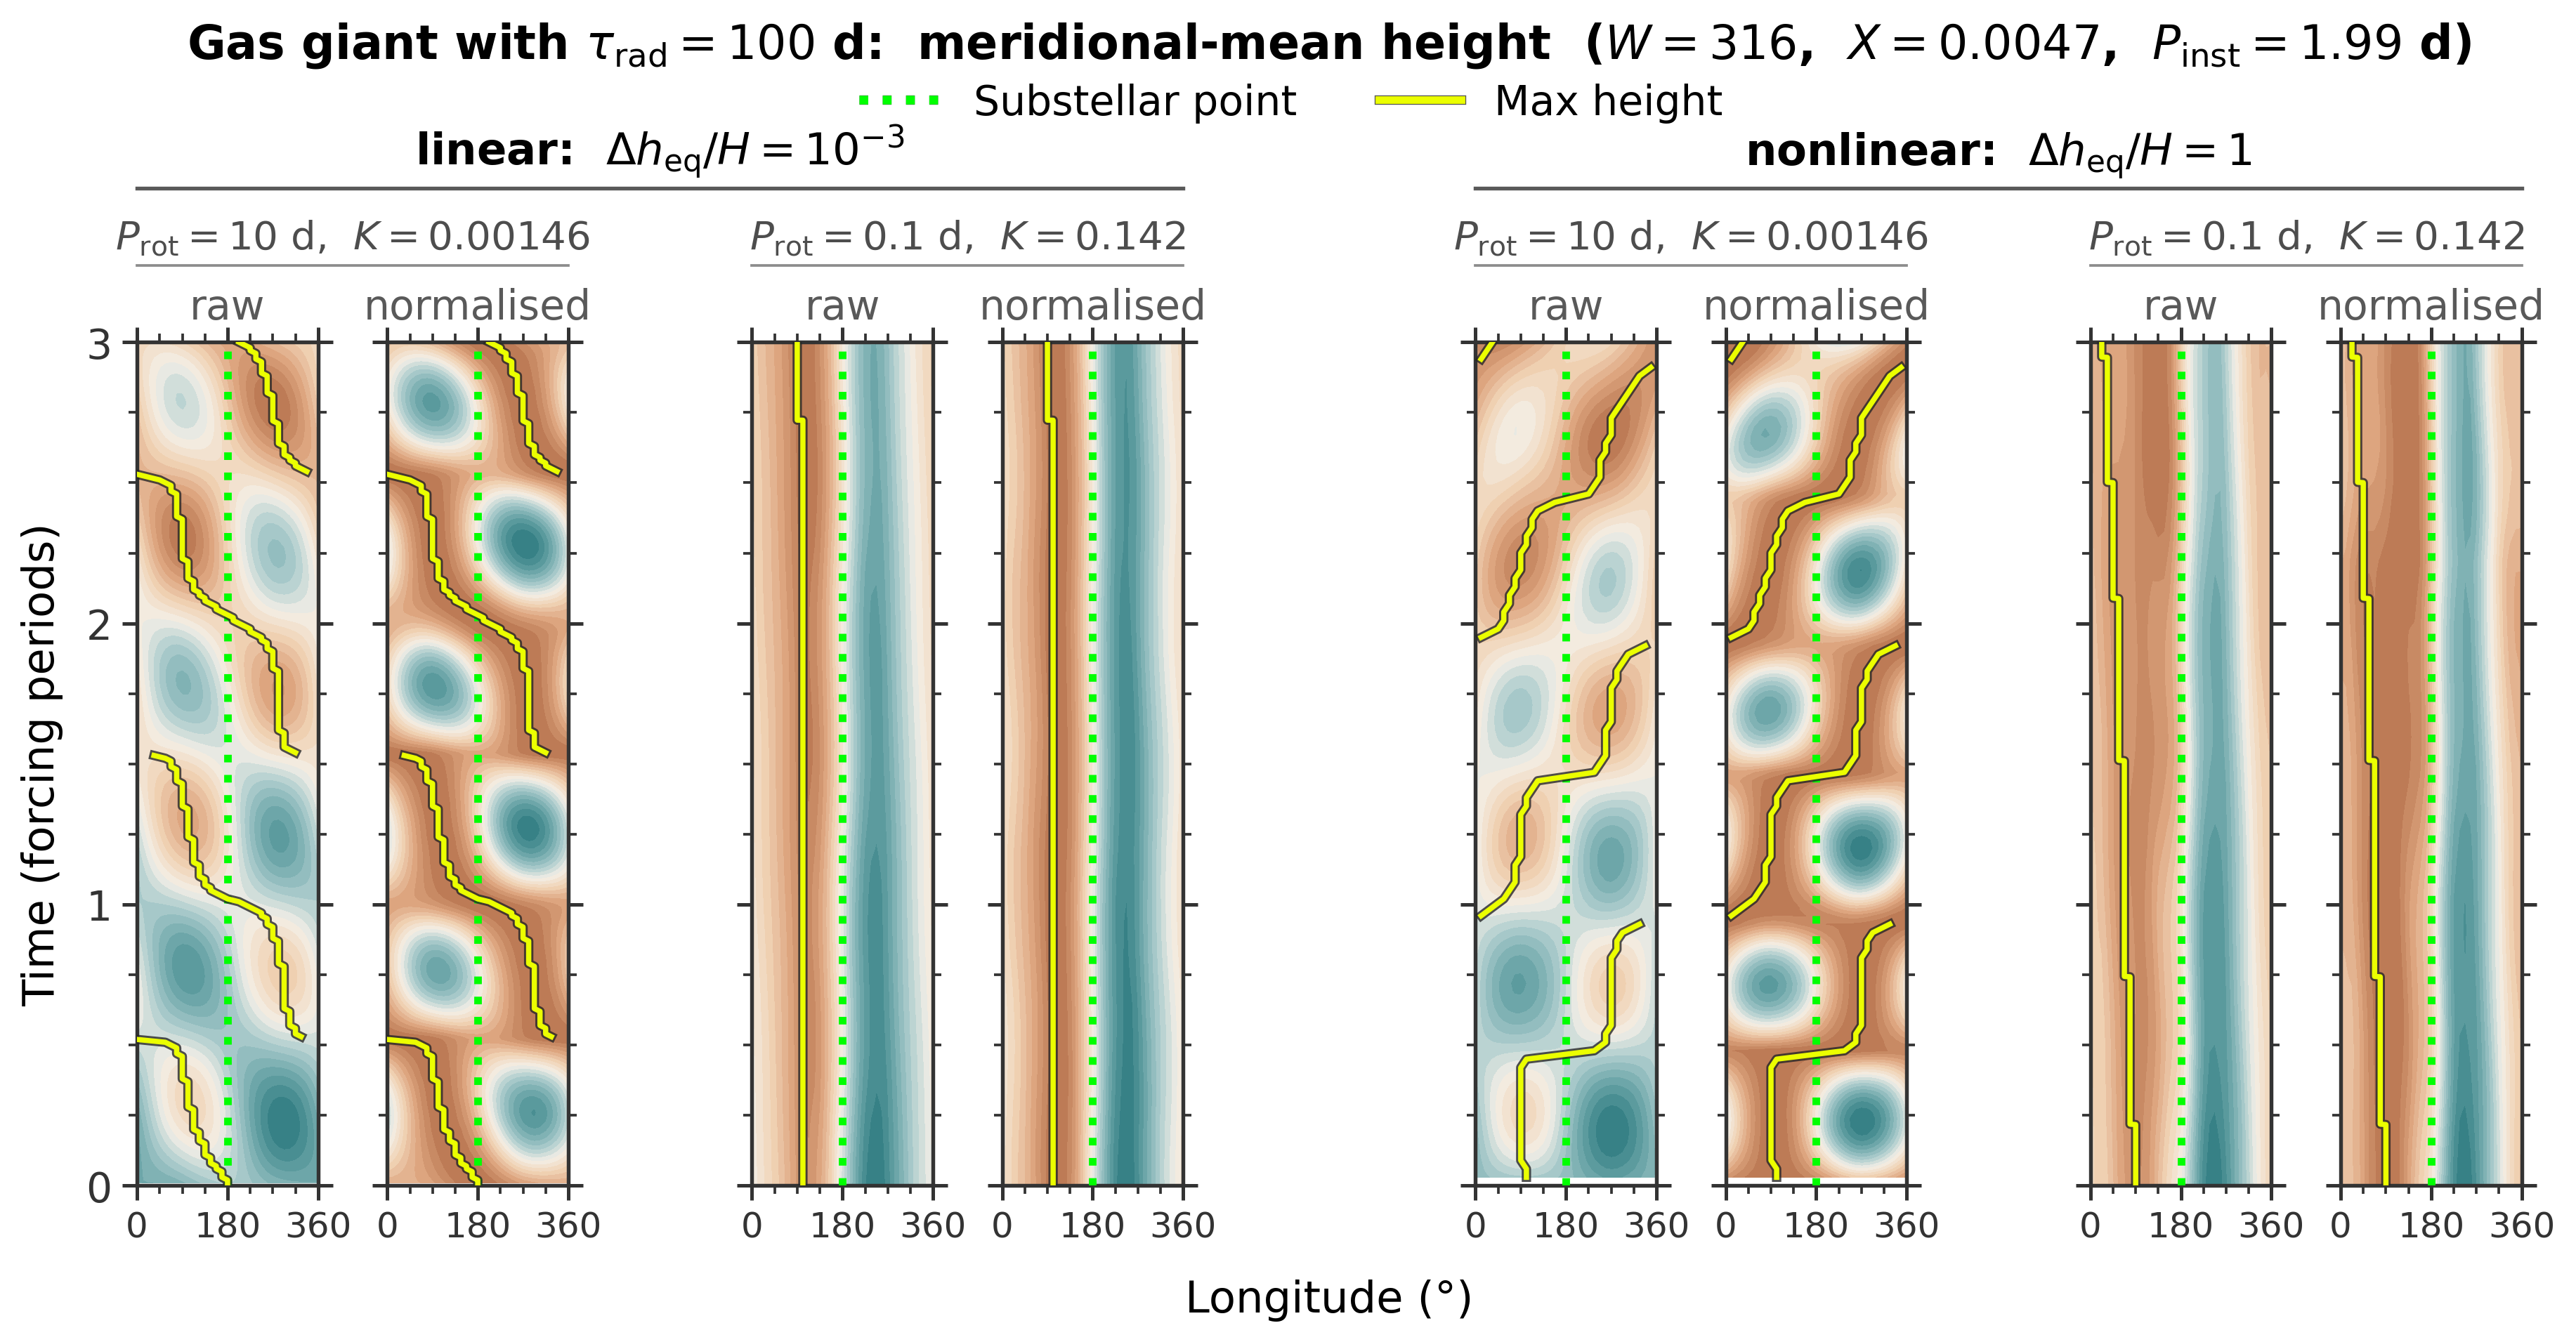
\includegraphics[width=\textwidth]{hovmoller_taurad100.png}
  \caption{Hovm\"oller diagrams of the meridional-mean height (averaged over
  $\pm45^\circ$ latitude) for the $\tau_{\rm rad} = 100\,$d gas giant, over the last
  three forcing periods. Each case is shown raw and normalised by its
  instantaneous maximum. Left group: linear forcing, $\Delta h_{\rm eq}/H = 10^{-3}$;
  right group: nonlinear, $\Delta h_{\rm eq}/H = 1$. Within each group the rotation
  rate increases from left to right, $P_{\rm rot} = 10\,$d ($K = 1.5\times10^{-3}$)
  and $0.1\,$d ($K = 0.14$). Dotted green marks the substellar meridian, yellow
  the longitude of maximum height. All four share $W = 316$, $X = 4.7\times10^{-3}$
  and $P_{\rm inst} = 1.99\,$d.}
  \label{fig:hov-taurad100}
\end{figure*}

Finally we note why the linear theory performs better than the size of $\varepsilon_h$ and
$\varepsilon_u$ might suggest. With the single mode ansatz of \S\ref{sec:first_order},
$h' = \Delta h\cos kx$ and $u' = g\tau_{\rm eff}\Delta h\,k \sin kx$, both neglected terms are
quadratic in a field of a single wavenumber and so project entirely onto the first overtone,
\begin{equation}
    \nabla\!\cdot\!\left(h'\mathbf{u}'\right) = g\tau_{\rm eff}\,\Delta h^{2} k^{2}\cos 2kx,
    \qquad
    \left(\mathbf{u}'\!\cdot\!\nabla\right)\mathbf{u}'
    = \tfrac{1}{2}\,\partial_x\!\left(u'^{2}\right) \propto \sin 2kx .
    \label{eq:app_harmonic}
\end{equation}
Neither has any projection onto the forced mode $k$. As long as $\varepsilon_h$ and
$\varepsilon_u$ are of order unity or smaller, the leading effect of nonlinearity is therefore
to generate a $2k$ structure with relative amplitude of order $\varepsilon$, while the
amplitude and phase of the fundamental are corrected only at order $\varepsilon^{2}$. The
clearest observational signature of a mildly violated linearity condition is thus additional
harmonic content in the phase curve rather than an error in the predicted day--night contrast.
The order of magnitude estimates of \S\ref{sec:app_caseI} and \S\ref{sec:app_caseII} become the
relevant description only once the corresponding $\varepsilon$ exceeds unity, where the
overtone is comparable to the fundamental and this ordering no longer applies.


\section{Response at long radiative timescale}
\label{app:long-taurad}

The two planets of Sec.~\ref{sec:sims} have $X \equiv \tau_{\rm wave}/\tau_{\rm rad}$
of order unity. Because $K \propto \tau_{\rm rad}^{-1}$ and $W \propto \tau_{\rm rad}$,
a much longer radiative timescale moves the system into a corner of the $K$--$W$
plane that those sweeps do not sample. To probe it we repeat the gas giant
($g = 10\,{\rm m\,s^{-2}}$, $a = 8.2\times10^{7}\,{\rm m}$, $H = 4\times10^{5}\,{\rm m}$,
$\tau_{\rm drag} = 3.89\times10^{6}\,{\rm s}$, $P_{\rm inst} = 1.99\,{\rm d}$)
with $\tau_{\rm rad} = 100\,$d instead of $0.1\,$d, holding the body, its drag and
its orbit fixed. This gives $X = 4.7\times10^{-3}$ and $W = 316$: the forcing
oscillates far faster than the atmosphere can relax. We run four cases spanning
the linear and nonlinear regimes ($\Delta h_{\rm eq}/H = 10^{-3}$ and $1$) and slow
and fast rotation ($P_{\rm rot} = 10\,$d and $0.1\,$d, i.e.\ $K = 1.5\times10^{-3}$
and $0.14$), integrating each for 40 forcing periods at the resolution of
Sec.~\ref{sec:sims} and diagnosing the last three.\footnote{The timestep must
resolve the rotation period as well as the forcing period; we take
$\Delta t = \min(P_{\rm inst}/100,\ 0.08\,{\rm d},\ P_{\rm rot}/100)$.}

Figure~\ref{fig:hov-taurad100} shows the outcome. Since $K \ll 1$ throughout, the
day--night contrast of the meridional-mean height is strongly suppressed,
reaching at most $4.3\%$ of $\Delta h_{\rm eq}$; the normalised panels are therefore
the informative ones. Two behaviours separate cleanly by rotation rate. At
$P_{\rm rot} = 10\,$d the height pattern does not lock to the substellar meridian
at all but circulates steadily, completing one circuit per forcing period
($2.04\,$d and $2.07\,$d against $P_{\rm inst} = 1.99\,$d) --- westward under weak
forcing and \emph{eastward} under strong forcing, the same sense reversal
reported in Sec.~\ref{sec:hovmoller} at $K = 1$. At $P_{\rm rot} = 0.1\,$d the
pattern is instead stationary (the $m=1$ crest drifts by less than
$1^\circ\,{\rm day}^{-1}$), locked $82^\circ$ west of substellar in the linear case
and $140^\circ$ west in the nonlinear one. Long radiative timescales thus do not
simply weaken the response: they admit a freely circulating state whose direction
is set by the forcing amplitude.




\section{Computation of the nondimensional parameters for observed systems}
\label{app:kw_calc}

This appendix sets out how $K$, $W$, $X$ and the forcing amplitude $F$ in Figure~\ref{fig:kw_planets} and Table~\ref{tab:kw_systems} are obtained. Planetary radii $R_{\rm p}$, masses, equilibrium temperatures $T_{\rm eq}$, orbital periods $P_{\rm orb}$ and eccentricities $e$ are the archival values from the NASA Exoplanet Archive composite-parameters table \citep{NEA2026}, adopted as published: no dayside or periastron rescaling is applied to $T_{\rm eq}$. The surface gravity follows from the archival mass and radius.

\subsection{Active-layer depth and the wave timescale}

The shallow-water layer depth $H$ is an equivalent depth rather than a measured quantity \citep{vallis2017atmospheric}. Instead of fixing it at one value for the whole sample, we set it per system to the pressure scale height evaluated at the planet's own equilibrium temperature,
\begin{equation}
    H = \frac{R_{\rm sp} T_{\rm eq}}{g}, \qquad R_{\rm sp} = \frac{\mathcal{R}}{\mu},
    \label{eq:app_H}
\end{equation}
with $\mu = 2.3$ for a solar-composition H/He atmosphere. This is consistent with the generic hot Jupiter of \cite{perez2013atmospheric}: at $g = 10\,\mathrm{m\,s^{-2}}$ and $T_{\rm eq} = 1600$~K, equation \eqref{eq:app_H} returns $H = 578$~km against their adopted $400$~km. Resulting depths across the sample range from $23$~km for the cool, high-gravity HAT-P-2b to ${\sim}1000$~km for the inflated WASP-118b.

Equation \eqref{eq:app_H} has a useful consequence. The gravity-wave speed becomes
\begin{equation}
    c = \sqrt{gH} = \sqrt{R_{\rm sp} T_{\rm eq}},
\end{equation}
independent of $g$, so that the wave timescale
\begin{equation}
    \tau_{\rm wave} = \frac{R_{\rm p}}{\sqrt{R_{\rm sp} T_{\rm eq}}}
    \label{eq:app_tauwave}
\end{equation}
depends only on the planetary radius and temperature. The radiative timescale of equation \eqref{eq:app_taurad}, however, carries a factor $1/g$ and therefore does depend on the planetary mass, so $X$, $K$ and $W$ are not mass-independent. For WASP-167b, whose mass is an upper limit rather than a measurement, the quoted $g$ is correspondingly an upper limit; its $\tau_{\rm rad}$ is then a lower limit and its $X$ and $K$ upper limits. It is retained on the diagram on that understanding.

The radiative timescale is the relaxation time of the weather layer cooling as a blackbody at its own equilibrium temperature, as in Appendix A of \cite{Banik2025},
\begin{equation}
    \tau_{\rm rad} = \frac{\Delta p}{g}\,\frac{c_{p}}{4\sigma T_{\rm eq}^{3}},
    \label{eq:app_taurad}
\end{equation}
with $\Delta p$ the thickness of the weather layer, $c_{p}$ the specific heat at constant pressure, and $\sigma$ the Stefan--Boltzmann constant. We take $\Delta p \simeq 10^{5}$~Pa, the photosphere depth appropriate to a hydrogen-dominated giant, and $c_{p} = 14.304$~kJ~K$^{-1}$~kg$^{-1}$, both following \cite{Banik2025}. $X = \tau_{\rm wave}/\tau_{\rm rad}$ follows directly.

This replaces the fitted scaling $\tau_{\rm rad}\approx 0.1\,(1600~\mathrm{K}/T_{\rm eq})^{3}$~days of \cite{perez2013atmospheric} used in an earlier version of this appendix, whose numerical coefficient corresponds to a particular unstated choice of $\Delta p$ and $g$. Equation \eqref{eq:app_taurad} is longer than that scaling by a factor of $0.5$--$47$ across the present sample (median $8.7$); because it depends on $g$ while the fitted scaling does not, the change is not a uniform rescaling and it reorders the systems in $X$, $K$ and $W$.

\subsection{Rotation, drag and $K$}

With $\tau_{\rm eff}^{-1} = \Omega + \tau_{\rm drag}^{-1}$ from \S\ref{sec:theory}, the heat-retention parameter is
\begin{equation}
    K = \frac{\tau_{\rm wave}^{2}}{\tau_{\rm rad}\tau_{\rm eff}}
      = X\,\tau_{\rm wave}\left(\Omega + \tau_{\rm drag}^{-1}\right).
    \label{eq:app_K}
\end{equation}
The drag timescale is unconstrained for every system in the sample. We therefore quote $K$ in the drag-free limit $\tau_{\rm drag}\to\infty$, where $K = X\,\tau_{\rm wave}\Omega$; because drag can only shorten $\tau_{\rm eff}$, this is a strict lower bound, and Figure~\ref{fig:kw_planets} shows the one-sided excursion to a strong-drag case, $\tau_{\rm drag} = 10^{4}$~s. Note that the ratio
\begin{equation}
    Z \equiv \frac{K}{X} = \tau_{\rm wave}\Omega
    \label{eq:app_Z}
\end{equation}
in this limit is independent of the assumed depth, since $\tau_{\rm wave} \propto H^{-1/2}$ appears once in $K/X$ only through $\Omega$; more precisely $Z \propto H^{-1/2}$ while $X \propto H^{-1/2}$ and $K \propto H^{-1}$, so the position of a system \emph{relative} to the $K = X$ boundary is less sensitive to $H$ than its absolute placement.

Rotation rates are assigned as follows. For circular orbits the planet is taken to rotate synchronously, $\Omega = 2\pi/P_{\rm orb}$. For eccentric orbits we use the pseudo-synchronous spin rate of \cite{Hut1981},
\begin{equation}
    \frac{\Omega_{\rm ps}}{n} = \frac{1 + \tfrac{15}{2}e^{2} + \tfrac{45}{8}e^{4} + \tfrac{5}{16}e^{6}}
                                     {\left(1 + 3e^{2} + \tfrac{3}{8}e^{4}\right)\left(1-e^{2}\right)^{3/2}},
    \label{eq:app_hut}
\end{equation}
with $n = 2\pi/P_{\rm orb}$. For HD~80606b this returns a spin period of $1.73$~d, consistent with the ${\sim}40$~h pseudo-synchronous period found by \cite{LangtonLaughlin2008}.

\subsection{Forcing period and amplitude}

The forcing period $T_{\rm instel}$ is set by the variability mechanism: the stellar pulsation period for category C, $P_{\rm orb}$ for the eccentric planets, and $P_{\rm orb}/2$ for category B. Every category-B system retained here is on a polar orbit, so the planet sweeps from one stellar pole to the equator and on to the other pole twice per orbit, encountering the full gravity-darkening contrast at half the orbital period. Then $W = 2\pi\tau_{\rm rad}/T_{\rm instel}$.

For the eccentric planets the fractional semi-amplitude of the forcing is computed from the orbit rather than assumed. The instellation scales as $r^{-2}$, so $T_{\rm eq}\propto r^{-1/2}$, and since the layer thickness is the temperature proxy,
\begin{equation}
    F = \frac{\sqrt{\rho}-1}{\sqrt{\rho}+1}, \qquad
    \rho = \frac{1+e}{1-e},
    \label{eq:app_F}
\end{equation}
giving $F = 0.13$--$0.68$ across the category-A sample. For the gravity-darkened hosts $F$ is the flux contrast swept along the transit chord, taken as ${\sim}0.10$ for KELT-9b \citep{Jones2022}. No such contrast has been published for MASCARA-1b, MASCARA-4b, TOI-1518b or WASP-189b, so these four are placed on the diagrams but omitted from the $FA$ ranking. For the pulsating hosts $F$ is the published pulsation amplitude in flux: ${\sim}3\times10^{-3}$ for WASP-33 \citep{vonEssen2020} and $200$~ppm for WASP-118 \citep{Temple2017}. No pulsation amplitude has been published for WASP-167, so it is placed on the diagram but omitted from the $FA$ ranking.

\subsection{Sample selection}

Categories B and C comprise the systems for which the relevant stellar variability has been detected and characterised: the gravity-darkened hosts KELT-9, MASCARA-1, MASCARA-4, TOI-1518 and WASP-189, and the pulsating hosts WASP-33, WASP-118 and WASP-167 \citep{Temple2017}. Category B is restricted to planets on polar orbits, for which the gravity-darkening cycle is actually swept: KELT-20b (MASCARA-2b) is excluded because its orbit is aligned with the stellar equator, so the planet remains at essentially one stellar latitude and sees no variation. HAT-P-56 is also a $\gamma$~Doradus pulsator, but its eccentricity of $0.29$ produces a forcing amplitude two orders of magnitude larger than its pulsation, so it is assigned to category A; each system is placed in the category of its dominant forcing.

The category-A sample is drawn from \cite{NEA2026} by requiring a transiting planet with
\begin{equation}
    e \geq 0.25,\quad R_{\rm p} \geq 0.8\,R_{\rm J},\quad T_{\rm eq} \geq 800~\mathrm{K},\quad
    3~\mathrm{d} \leq P_{\rm orb} \leq 25~\mathrm{d}.
\end{equation}
The radius and temperature cuts keep the sample within the giant-planet regime where the shallow-water framework and equation \eqref{eq:app_taurad} are appropriate. The lower period bound rejects ultra-short-period orbits whose reported eccentricities are unlikely to survive tidal circularisation; the upper bound keeps the sample within the range where pseudo-synchronous rotation is plausible. This yields sixty systems. HD~80606b ($P_{\rm orb} = 111$~d) is retained as an explicit exception because its pseudo-synchronous spin is established observationally \citep{LangtonLaughlin2008}; it should be understood as the one system in the sample whose rotation state rests on more than the assumption of equation \eqref{eq:app_hut}.

Circumbinary planets, which form a natural fourth category of variably irradiated system, are omitted altogether. Their rotation states are unknown --- tidal synchronisation timescales at their orbital separations exceed the system ages --- and since $\Omega$ enters $K$ directly through $\tau_{\rm eff}$, no defensible value of $K$ can be computed for them.

\subsection{Caveats}

Identifying the active-layer depth with a single pressure scale height is a choice, not a derivation; equivalent depths of several scale heights are equally defensible, and since $X \propto H^{-1/2}$ and $K \propto H^{-1}$, a factor of a few in $H$ displaces every point. As noted above, the clustering near $K = X$ is more robust than the absolute placements. The mean molecular weight $\mu = 2.3$ is applied uniformly, but H$_2$ is substantially dissociated on KELT-9b and WASP-33b; taking $\mu \to 1.3$ there would raise $H$ by $77\%$, lowering $X$ by ${\sim}1.3$ and $K$ by ${\sim}1.8$, which does not change their regime assignment. Finally, the archival $T_{\rm eq}$ for the eccentric planets is orbit-averaged and so understates the periastron instellation; this is internally consistent with the large $F$ that equation \eqref{eq:app_F} assigns them, but for the most eccentric cases ($F \to 0.7$ for HD~80606b) the linear-forcing assumption behind equation \eqref{eq:so_amp} is strained, and the tabulated $A$ should be read as indicative only.

\begin{deluxetable*}{llccccccccccc}
\tabletypesize{\tiny}
\tablecaption{Nondimensional placement of the sixty-eight variably irradiated systems of Figure~\ref{fig:kw_planets}, ordered by category and then by observable modulation $FA$. Categories: A = eccentric orbit, B = gravity-darkened host, C = pulsating host, each system assigned to the category of its dominant forcing. Columns: equilibrium temperature and radius from \cite{NEA2026}; eccentricity; forcing period; active-layer depth from equation \eqref{eq:app_H}; $X = \tau_{\rm wave}/\tau_{\rm rad}$ with $\tau_{\rm wave}$ from equation \eqref{eq:app_tauwave} with $\tau_{\rm rad}$ from equation \eqref{eq:app_taurad}; $K$ in the drag-free limit, equation \eqref{eq:app_K}, hence a lower bound; $W = 2\pi\tau_{\rm rad}/T_{\rm instel}$; the normalised amplitude $A \equiv \Delta h_{\rm amp}/(F\Delta h_{\rm eq})$ from equation \eqref{eq:so_amp} evaluated at each system's own $(K, W, X)$; the forcing amplitude $F$, computed from the orbit via equation \eqref{eq:app_F} for category A and taken from the literature for B and C; and their product $FA$, the predicted observable modulation. \label{tab:kw_systems}}
\tablewidth{0pt}
\tablehead{
  \colhead{System} & \colhead{Cat.} & \colhead{$T_{\rm eq}$} & \colhead{$R_{\rm p}$} &
  \colhead{$e$} & \colhead{$T_{\rm instel}$} & \colhead{$H$} &
  \colhead{$X$} & \colhead{$K$} & \colhead{$W$} &
  \colhead{$A$} & \colhead{$F$} & \colhead{$FA$} \\
  \colhead{} & \colhead{} & \colhead{(K)} & \colhead{($R_{\rm J}$)} &
  \colhead{} & \colhead{(d)} & \colhead{(km)} & & & & & &
}
\startdata
WASP-33b & C & 2782 & 1.59 & \nodata & 0.0476 & 492 & 21.84 & 46.77 & 2.512 & 0.37 & 0.003 & 0.0011 \\
WASP-118b & C & 1729 & 1.44 & \nodata & 1.9 & 1017 & 6.01 & 4.45 & 0.262 & 0.95 & $2\times10^{-4}$ & $1.9\times10^{-4}$ \\
WASP-167b & C & 2329 & 1.58 & \nodata & 0.167 & 106 & 13.90 & 19.46 & 1.222 & 0.63 & \nodata & \nodata \\
KELT-9b & B & 3921 & 1.94 & \nodata & 0.741 & 744 & 62.62 & 113.04 & 0.058 & 1.00 & 0.100 & 0.0997 \\
KELT-20b & B & 2262 & 1.74 & \nodata & 0.45 & 296 & 14.24 & 12.97 & 0.494 & 0.90 & 0.050 & 0.0450 \\
HATS-27b & A & 1659 & 1.50 & 0.581 & 4.64 & 1027 & 5.65 & 14.65 & 0.122 & 0.94 & 0.320 & 0.2997 \\
TIC~183374187b & A & 1379 & 1.25 & 0.506 & 5.06 & 563 & 2.97 & 4.90 & 0.194 & 0.84 & 0.272 & 0.2285 \\
HATS-50b & A & 1275 & 1.13 & 0.516 & 3.83 & 609 & 2.21 & 4.67 & 0.324 & 0.82 & 0.278 & 0.2278 \\
HATS-10b & A & 1407 & 0.97 & 0.501 & 3.31 & 366 & 2.42 & 4.59 & 0.279 & 0.83 & 0.269 & 0.2216 \\
HAT-P-2b & A & 1540 & 0.95 & 0.517 & 5.63 & 23 & 2.97 & 3.29 & 0.125 & 0.79 & 0.279 & 0.2189 \\
Kepler-427b & A & 1100 & 1.23 & 0.570 & 10.3 & 837 & 1.66 & 1.87 & 0.188 & 0.67 & 0.313 & 0.2089 \\
HATS-46b & A & 1054 & 0.90 & 0.559 & 4.74 & 725 & 1.09 & 1.92 & 0.463 & 0.66 & 0.306 & 0.2017 \\
HAT-P-34b & A & 1520 & 1.20 & 0.432 & 5.45 & 95 & 3.62 & 3.97 & 0.134 & 0.83 & 0.227 & 0.1876 \\
TOI-615b & A & 1666 & 1.69 & 0.390 & 4.66 & 1601 & 6.44 & 9.85 & 0.119 & 0.92 & 0.203 & 0.1873 \\
TOI-2005b & A & 1221 & 1.07 & 0.597 & 17.3 & 32 & 1.87 & 1.15 & 0.082 & 0.55 & 0.331 & 0.1820 \\
HATS-41b & A & 1710 & 1.33 & 0.380 & 4.19 & 45 & 5.40 & 6.92 & 0.123 & 0.90 & 0.197 & 0.1769 \\
HD~17156b & A & 888 & 1.09 & 0.677 & 21.2 & 48 & 0.86 & 0.75 & 0.173 & 0.43 & 0.390 & 0.1696 \\
TOI-1994b & A & 2290 & 1.22 & 0.341 & 4.03 & 22 & 10.29 & 9.74 & 0.053 & 0.93 & 0.176 & 0.1632 \\
HATS-11b & A & 1596 & 1.61 & 0.340 & 3.62 & 726 & 5.50 & 9.15 & 0.175 & 0.92 & 0.175 & 0.1608 \\
CoRoT-20b & A & 1024 & 0.84 & 0.590 & 9.24 & 25 & 0.95 & 0.91 & 0.259 & 0.49 & 0.326 & 0.1607 \\
HD~80606b & A & 405 & 1.03 & 0.932 & 111 & 15 & 0.11 & 0.29 & 0.348 & 0.23 & 0.684 & 0.1547 \\
HATS-40b & A & 2101 & 1.58 & 0.312 & 3.26 & 481 & 10.74 & 15.75 & 0.085 & 0.95 & 0.160 & 0.1528 \\
HATS-51b & A & 1553 & 1.41 & 0.330 & 3.35 & 586 & 4.50 & 7.00 & 0.205 & 0.90 & 0.170 & 0.1523 \\
TIC~237913194b & A & 974 & 1.12 & 0.575 & 15.2 & 91 & 1.11 & 0.84 & 0.184 & 0.47 & 0.316 & 0.1494 \\
TOI-677b & A & 1252 & 1.17 & 0.460 & 11.2 & 203 & 2.18 & 1.36 & 0.117 & 0.61 & 0.244 & 0.1490 \\
WASP-150b & A & 1460 & 1.07 & 0.378 & 5.64 & 29 & 2.93 & 2.41 & 0.147 & 0.75 & 0.196 & 0.1477 \\
TOI-6628b & A & 833 & 0.98 & 0.670 & 18.2 & 158 & 0.66 & 0.59 & 0.245 & 0.38 & 0.385 & 0.1461 \\
HATS-53b & A & 1312 & 1.34 & 0.330 & 3.85 & 577 & 2.81 & 3.92 & 0.296 & 0.83 & 0.170 & 0.1412 \\
HATS-8b & A & 1324 & 0.87 & 0.376 & 3.58 & 1066 & 1.87 & 2.07 & 0.309 & 0.72 & 0.195 & 0.1410 \\
HAT-P-56b & A & 1840 & 1.51 & 0.290 & 2.79 & 265 & 7.37 & 12.21 & 0.148 & 0.94 & 0.148 & 0.1394 \\
TOI-5301b & A & 1648 & 1.17 & 0.330 & 5.86 & 88 & 4.33 & 3.09 & 0.098 & 0.81 & 0.170 & 0.1369 \\
TOI-622b & A & 1388 & 0.82 & 0.420 & 6.4 & 454 & 1.99 & 1.29 & 0.150 & 0.61 & 0.220 & 0.1337 \\
XO-3b & A & 1890 & 1.32 & 0.279 & 3.19 & 36 & 6.89 & 8.38 & 0.119 & 0.92 & 0.142 & 0.1314 \\
WASP-186b & A & 1378 & 1.11 & 0.330 & 5.03 & 59 & 2.63 & 2.28 & 0.195 & 0.75 & 0.170 & 0.1282 \\
TIC~393818343b & A & 806 & 1.09 & 0.606 & 16.2 & 32 & 0.67 & 0.57 & 0.303 & 0.38 & 0.337 & 0.1271 \\
HATS-39b & A & 1645 & 1.57 & 0.275 & 4.58 & 939 & 5.79 & 6.20 & 0.126 & 0.90 & 0.140 & 0.1262 \\
TOI-4603b & A & 1677 & 1.04 & 0.325 & 7.25 & 21 & 4.03 & 2.03 & 0.075 & 0.73 & 0.167 & 0.1221 \\
CoRoT-16b & A & 1196 & 1.17 & 0.330 & 5.35 & 446 & 1.94 & 1.79 & 0.281 & 0.71 & 0.170 & 0.1201 \\
TOI-6019b & A & 1095 & 1.10 & 0.480 & 14.5 & 410 & 1.46 & 0.76 & 0.135 & 0.46 & 0.256 & 0.1175 \\
HAT-P-60b & A & 1772 & 1.63 & 0.250 & 4.79 & 1198 & 7.24 & 6.99 & 0.096 & 0.91 & 0.127 & 0.1161 \\
HATS-62b & A & 1237 & 1.05 & 0.298 & 3.28 & 1122 & 1.91 & 2.34 & 0.415 & 0.76 & 0.152 & 0.1155 \\
HD~118203b & A & 1361 & 1.14 & 0.314 & 6.13 & 121 & 2.62 & 1.84 & 0.166 & 0.72 & 0.161 & 0.1153 \\
TOI-2025b & A & 1166 & 1.06 & 0.394 & 8.87 & 53 & 1.65 & 1.01 & 0.183 & 0.55 & 0.205 & 0.1135 \\
TOI-3464b & A & 1693 & 1.23 & 0.250 & 3.65 & 298 & 4.87 & 4.75 & 0.145 & 0.88 & 0.127 & 0.1115 \\
Kepler-425b & A & 1070 & 0.98 & 0.330 & 3.8 & 597 & 1.23 & 1.41 & 0.553 & 0.65 & 0.170 & 0.1100 \\
K2-132b & A & 1586 & 1.30 & 0.290 & 9.18 & 798 & 4.38 & 2.04 & 0.070 & 0.74 & 0.148 & 0.1098 \\
TOI-150b & A & 1404 & 1.25 & 0.262 & 5.86 & 129 & 3.12 & 2.19 & 0.159 & 0.77 & 0.133 & 0.1020 \\
TOI-172b & A & 1198 & 0.96 & 0.381 & 9.48 & 30 & 1.61 & 0.79 & 0.158 & 0.49 & 0.198 & 0.0975 \\
HAT-P-31b & A & 1450 & 1.09 & 0.250 & 5.01 & 111 & 2.93 & 2.00 & 0.169 & 0.75 & 0.127 & 0.0955 \\
WASP-162b & A & 910 & 1.00 & 0.434 & 9.62 & 26 & 0.84 & 0.57 & 0.355 & 0.40 & 0.228 & 0.0915 \\
TOI-4914b & A & 894 & 1.15 & 0.408 & 10.6 & 241 & 0.92 & 0.60 & 0.340 & 0.42 & 0.213 & 0.0901 \\
WASP-8b & A & 1059 & 1.13 & 0.310 & 8.16 & 78 & 1.39 & 0.81 & 0.266 & 0.53 & 0.159 & 0.0835 \\
TOI-5027b & A & 1056 & 0.96 & 0.385 & 10.2 & 70 & 1.17 & 0.57 & 0.213 & 0.41 & 0.200 & 0.0820 \\
TOI-3919b & A & 1198 & 1.10 & 0.259 & 7.43 & 54 & 1.83 & 0.96 & 0.201 & 0.58 & 0.132 & 0.0765 \\
TOI-1842b & A & 1200 & 1.10 & 0.276 & 9.57 & 756 & 1.85 & 0.78 & 0.156 & 0.52 & 0.141 & 0.0730 \\
TOI-2416b & A & 1080 & 0.88 & 0.320 & 8.28 & 41 & 1.13 & 0.52 & 0.247 & 0.40 & 0.164 & 0.0663 \\
WASP-117b & A & 1001 & 1.06 & 0.300 & 10 & 547 & 1.13 & 0.51 & 0.256 & 0.40 & 0.154 & 0.0620 \\
HAT-P-17b & A & 800 & 1.05 & 0.350 & 10.3 & 222 & 0.64 & 0.35 & 0.486 & 0.31 & 0.181 & 0.0558 \\
HD~1397b & A & 1228 & 1.03 & 0.251 & 11.5 & 454 & 1.82 & 0.55 & 0.120 & 0.43 & 0.128 & 0.0553 \\
KOI-12b & A & 911 & 1.23 & 0.340 & 17.9 & 183 & 1.04 & 0.35 & 0.191 & 0.30 & 0.175 & 0.0533 \\
TOI-558b & A & 1061 & 1.09 & 0.298 & 14.6 & 51 & 1.34 & 0.41 & 0.148 & 0.35 & 0.152 & 0.0528 \\
K2-287b & A & 804 & 0.85 & 0.478 & 14.9 & 267 & 0.52 & 0.24 & 0.332 & 0.21 & 0.254 & 0.0528 \\
K2-232b & A & 1030 & 1.00 & 0.258 & 11.2 & 377 & 1.14 & 0.39 & 0.211 & 0.35 & 0.131 & 0.0454 \\
Kepler-643b & A & 963 & 0.91 & 0.370 & 16.3 & 114 & 0.88 & 0.25 & 0.176 & 0.23 & 0.192 & 0.0444 \\
K2-261b & A & 1036 & 0.83 & 0.274 & 11.6 & 476 & 0.96 & 0.27 & 0.199 & 0.26 & 0.140 & 0.0362 \\

\enddata
\end{deluxetable*}


% \section{Setting up boundaries for physical parameters}
% Trying to Figure out how to restrict the domain of simulations' parameters to the 
% domain of physical quantities.
% Let's say we have a set of dimensionless quantities $L_1, ... L_k$ in $n$-dimensional space.
% $n \ge k$.
% Let's say we have restrictions on the domain in the physical space $x^1, ..., x^n$,
% with constraints on $x^i$ being $x^i_{max/min}$.
% Let's say we are going to start from initial point $x_i = 0, L_i = 0 \forall i$, and
% we want to change in the direction $L_1$.
% So our $L_1$ change vector will be $(1, 0, ..., 0)$ in $L-$space.
% Matrix $A$ to convert between vector $u$ of $x-$space and vector $v$ of $L-$space
% is defined for $k$ rows, with $i^{\text{th}}$ row corresponding to matrix representation
% of $L_i$ in $x-$space basis.
% So we have freedom in choosing $n-k$ vectors. We call these vectors \textbf{free vectors}.
% Finding $x-$space vector from a given $L-$space vector can be done via $v = A^{-1} u$,
% assuming we have chosen free $L-$vectors and added them to $A$ in such a way that
% $A$ is invertible.

% If we choose those free vectors at random, we run into an issue when sometimes our
% $x$-space vector lies outside of our allowed $x-$space domain.
% In order to avoid this issue, we need to Figure out how to choose the free vectors in
% a way that will force our $A^{-1}$ to place all the vectors in the domain, assuming
% it is possible. Doing that first requires finding out what are possible attainable
% maximum values of $L_1$ assuming fixed $L_2, ..., L_k$.

% We start by fixing $L_2, ..., L_k$. This gives us a subspace $S$ of dimension $k-1$, 
% that should be passing through the origin. HOW TO DO IT? NOT SURE...
% After we fixed those parameters, we look at our $L_1$ vector in $x-$space.

% We find projection of $L_1$ onto $S$, which gives us the direction of increase of 
% $L_1$ values (normal vector) in the subspace $S$.
% We then find out all intersections of $S$ subspace with each of the boundaries
% in $x-$space. Each of those will correspond to a subspace $B_i$
% of dimensionality $k-2$. ALSO NOT SURE HOW TO DO THIS.
% For each of those existing intersections, we calculate the outwards-pointing normal vector
% (i.e. the normal vector pointing outwards from the starting point, i.e. origin).

% % BELOW PARAGRAPH WAS WRONG
% %We then look at each of the subspaces, corresponding to boundaries
% %in $x-$space. Each of those will correspond to a subspace $B_i$
% %of dimensionality $n-1$. ALSO NOT SURE HOW TO DO THIS.
% %For each of $B_i$, we calculate the outwards-pointing normal vector
% %(the normal vector pointing outwards from the starting point, i.e. origin).

% Assuming box-like boundaries, i.e. just min/max allowed values,
% we then will have 2 normal vectors for each of the dimension: one for min, one for max.
% We then will calculate the dot product with vector $L_1$.
% If we JUST have box-like boundaries, can just find which of the components are positive 
% and which ones are negative for $L_1$.
% But if we have a skewed boundaries (i.e. $x+y = max$), then MUST do dot product.

% Then for each of the dot product being positive, it means that the max value of $L_1$
% will "touch" that boundary.
% i.e. if $L_1 = (1, -2, 3)$, then max value is attained at max of $x,z$ and min of $y$.
% If we get 0, then any point in a subspace along that subspace will work.
% For instacne, if $L_1 = (1, -2, 0)$, then max value is attained at max of $x$, 
% min of $y$, and any value $z$ withing the bondary.

% We then find out which of the coordinates intersect with our subspace $S$.
% Those coordinates we take as their proper max/min values. For all other 
% coordinates which do not intersect, we find their values from solving a system,
% assuming that the point of interest lies in $S$. ALSO NOT SURE HOW TO DO THIS. VERY NOT SURE.

% We then can set up the point at which the max value is attained in $x-$space from our 
% previous calculations. Vector pointing in that direction we normalize and call $N$.

% Next step is to construct free vectors $F_i$, so that together 
% $\left( L_1, ..., L_k, F_1, ..., F_{n-k} \right) = A^T$.

% In order to do this, we must make sure that, since we're only changing vector $N$,
% all free parameters vectors stay the same after we change $N$.
% This is only guaranteed if $F_i \perp n, \forall i$.
% Thus we construct basis $\left< F_i \right>$, that is orthogonal to all $N$.
% This is not enough though -- too many free parameters, since we only cover $n-k+1$
% out of $N$ possible dimensions. Where do we take the other $k-1$ vectors
% to help us constrain $F_i$?

% $F_i$ should also not change if we are walking through $S$.
% So we zero-out all $L_i, i \neq 1$ components, and thus we have a basis:
% $\left< L' \right> = n, L_i, i \neq 1$.

% Finally, we can orthogonalize our $F_i$ vectors:
% \[
% 	F_i^* = F_i - \sum_{j} \frac{F_i \cdot L'_j}{\left| F_i \right| \left| L'_j \right|} L'_j
% \]
% While $F_i$ might not be orthogonal between each other, they are orthogonal to all of
% $\left< L' \right>$ basis vectors.

% We then must construct a new matrix for every new direction of increase in 
% directional sampling, including the direction of minimum instead of maximum.


%% For this sample we use BibTeX plus aasjournalv7.bst to generate the
%% the bibliography. The sample7.bib file was populated from ADS. To
%% get the citations to show in the compiled file do the following:
%%
%% pdflatex sample7.tex
%% bibtext sample7
%% pdflatex sample7.tex
%% pdflatex sample7.tex

\bibliography{sample7}{}
\bibliographystyle{aasjournalv7}

%% This command is needed to show the entire author+affiliation list when
%% the collaboration and author truncation commands are used.  It has to
%% go at the end of the manuscript.
%\allauthors

%% Include this line if you are using the \added, \replaced, \deleted
%% commands to see a summary list of all changes at the end of the article.
%\listofchanges

\end{document}

% End of file `sample7.tex'.
